%%
%% This is file `sample-acmsmall-submission.tex',
%% generated with the docstrip utility.
%%
%% The original source files were:
%%
%% samples.dtx  (with options: `all,journal,bibtex,acmsmall-submission')
%% 
%% IMPORTANT NOTICE:
%% 
%% For the copyright see the source file.
%% 
%% Any modified versions of this file must be renamed
%% with new filenames distinct from sample-acmsmall-submission.tex.
%% 
%% For distribution of the original source see the terms
%% for copying and modification in the file samples.dtx.
%% 
%% This generated file may be distributed as long as the
%% original source files, as listed above, are part of the
%% same distribution. (The sources need not necessarily be
%% in the same archive or directory.)
%%
%%
%% Commands for TeXCount
%TC:macro \cite [option:text,text]
%TC:macro \citep [option:text,text]
%TC:macro \citet [option:text,text]
%TC:envir table 0 1
%TC:envir table* 0 1
%TC:envir tabular [ignore] word
%TC:envir displaymath 0 word
%TC:envir math 0 word
%TC:envir comment 0 0
%%
%% The first command in your LaTeX source must be the \documentclass
%% command.
%%
%% For submission and review of your manuscript please change the
%% command to \documentclass[manuscript, screen, review]{acmart}.
%%
%% When submitting camera ready or to TAPS, please change the command
%% to \documentclass[sigconf]{acmart} or whichever template is required
%% for your publication.
%%
%%
\documentclass[acmsmall,screen]{acmart}
%%
\usepackage[T1]{fontenc}
\usepackage[utf8]{inputenc}
\usepackage{lmodern}
\usepackage{xcolor}
\usepackage{graphicx}
\usepackage{booktabs}
\usepackage{longtable}
\usepackage{tabularx}
\usepackage{array}
\usepackage{hyperref}
\usepackage{enumitem}
\usepackage{amsmath}
\usepackage{pdflscape}
\usepackage{multirow}
\usepackage{caption}

\setlength{\textfloatsep}{8pt plus 2pt minus 2pt}
\setlength{\floatsep}{8pt plus 2pt minus 2pt}
\setlength{\intextsep}{8pt plus 2pt minus 2pt}
\captionsetup{skip=4pt}
\renewcommand{\topfraction}{0.9}
\renewcommand{\bottomfraction}{0.8}
\renewcommand{\textfraction}{0.07}
\renewcommand{\floatpagefraction}{0.75}
\setcounter{topnumber}{3}
\setcounter{bottomnumber}{2}
\setcounter{totalnumber}{5}

%% \BibTeX command to typeset BibTeX logo in the docs
\AtBeginDocument{%
  \providecommand\BibTeX{{%
    Bib\TeX}}}

%% Rights management information.  This information is sent to you
%% when you complete the rights form.  These commands have SAMPLE
%% values in them; it is your responsibility as an author to replace
%% the commands and values with those provided to you when you
%% complete the rights form.
\setcopyright{acmlicensed}
\copyrightyear{2018}
\acmYear{2018}
\acmDOI{XXXXXXX.XXXXXXX}

%%
%% These commands are for a JOURNAL article.
\acmJournal{JACM}
\acmVolume{37}
\acmNumber{4}
\acmArticle{111}
\acmMonth{8}

%%
%% Submission ID.
%% Use this when submitting an article to a sponsored event. You'll
%% receive a unique submission ID from the organizers
%% of the event, and this ID should be used as the parameter to this command.
%%\acmSubmissionID{123-A56-BU3}

%%
%% For managing citations, it is recommended to use bibliography
%% files in BibTeX format.
%%
%% You can then either use BibTeX with the ACM-Reference-Format style,
%% or BibLaTeX with the acmnumeric or acmauthoryear sytles, that include
%% support for advanced citation of software artefact from the
%% biblatex-software package, also separately available on CTAN.
%%
%% Look at the sample-*-biblatex.tex files for templates showcasing
%% the biblatex styles.
%%

%%
%% The majority of ACM publications use numbered citations and
%% references.  The command \citestyle{authoryear} switches to the
%% "author year" style.
%%
%% If you are preparing content for an event
%% sponsored by ACM SIGGRAPH, you must use the "author year" style of
%% citations and references.
%% Uncommenting
%% the next command will enable that style.
%%\citestyle{acmauthoryear}


%%
%% end of the preamble, start of the body of the document source.
\begin{document}

%%
%% The "title" command has an optional parameter,
%% allowing the author to define a "short title" to be used in page headers.
\title{BearWave: An Open-Source Low-Power HF/NVIS Monitoring System for Remote Conservation}

%%
%% The "author" command and its associated commands are used to define
%% the authors and their affiliations.
%% Of note is the shared affiliation of the first two authors, and the
%% "authornote" and "authornotemark" commands
%% used to denote shared contribution to the research.
\author{Mark Butterworth}
%\orcid{0000-0002-2998-5056}
\affiliation{%
  \institution{ Cardiff University}
  % \streetaddress{Cathays}
  % \city{Cardiff}
   \country{United Kingdom}
  % \postcode{CF10 3AT}
}
\email{ButterworthMA@cardiff.ac.uk}

\author{Omer Rana}
\affiliation{%
  \institution{Cardiff University}
  % \streetaddress{Cathays}
  % \city{Cardiff}
  \country{United Kingdom}
  % \postcode{CF10 3AT}
}
\email{ranaof@cardiff.ac.uk}

\author{Pablo Orozco-terWengel}
\affiliation{%
  \institution{ Cardiff University}
  % \streetaddress{Cathays}
  % \city{Cardiff}
  \country{United Kingdom}
}
\email{orozco-terwengelpa@cardiff.ac.uk}

\author{Beno{\^i}t Goossens}
\affiliation{%
  \institution{ Cardiff University}
  % \streetaddress{Cathays}
  % \city{Cardiff}
  \country{United Kingdom}
}
\email{goossensbr@cardiff.ac.uk}

\author{Charith Perera}
\affiliation{%
  \institution{ Cardiff University}
  % \streetaddress{Cathays}
  % \city{Cardiff}
  \country{United Kingdom}
}
\email{pererac@cardiff.ac.uk}


%%
%% By default, the full list of authors will be used in the page
%% headers. Often, this list is too long, and will overlap
%% other information printed in the page headers. This command allows
%% the author to define a more concise list
%% of authors' names for this purpose.
\renewcommand{\shortauthors}{Butterworth et al.}

%%
%% The abstract is a short summary of the work to be presented in the
%% article.
\begin{abstract}
Remote conservation sites often require reliable alerts from traps, camera stations, and environmental sensors in places where terrestrial communications infrastructure is absent and satellite communication is expensive or power intensive. This paper presents BearWave as an open-source and open-hardware monitoring system for conservation organisations that need to build, maintain, and adapt their own low-bandwidth field infrastructure. Building on earlier work that validated Near Vertical Incidence Skywave (NVIS) communication for rainforest monitoring, this paper focuses on the complete deployable system: the control node, the remote node hardware, the ESP32 supervisory firmware, the Raspberry Pi software, the compact message format used to convert local sensor events into long-haul HF alerts, and an alarm-triggered slow-scan television (SSTV) still-image extension for visual verification. The primary system function remains reliable low-power alarm messaging; image transfer is treated as optional best-effort context rather than as the authoritative alarm channel. The manuscript is structured as a reproducible system paper in the style of open ecological hardware reports, documenting design rationale, assembly and validation requirements, power-management strategy, operating modes, operator display, image workflow, and deployment constraints. 
\end{abstract}

%%
%% The code below is generated by the tool at http://dl.acm.org/ccs.cfm.
%% Please copy and paste the code instead of the example below.
%%
\begin{CCSXML}
<ccs2012>
 <concept>
  <concept_id>10003033.10003083.10003014</concept_id>
  <concept_desc>Networks~Wireless access networks</concept_desc>
  <concept_significance>500</concept_significance>
 </concept>
 <concept>
  <concept_id>10010520.10010521.10010542</concept_id>
  <concept_desc>Computer systems organization~Sensor networks</concept_desc>
  <concept_significance>500</concept_significance>
 </concept>
 <concept>
  <concept_id>10010583.10010662.10010674</concept_id>
  <concept_desc>Hardware~Sensor applications and deployments</concept_desc>
  <concept_significance>300</concept_significance>
 </concept>
 <concept>
  <concept_id>10010405.10010444.10010449</concept_id>
  <concept_desc>Applied computing~Environmental sciences</concept_desc>
  <concept_significance>300</concept_significance>
 </concept>
</ccs2012>
\end{CCSXML}

\ccsdesc[500]{Networks~Wireless access networks}
\ccsdesc[500]{Computer systems organization~Sensor networks}
\ccsdesc[300]{Hardware~Sensor applications and deployments}
\ccsdesc[300]{Applied computing~Environmental sciences}

%%
%% Keywords. The author(s) should pick words that accurately describe
%% the work being presented. Separate the keywords with commas.
\keywords{conservation technology, open hardware, sensor networks, HF communication, NVIS, slow-scan television, low-power systems, wildlife monitoring, remote sensing, image verification}

%\received{DD Month YYYY}
%\received[revised]{DD Month YYYY}
%\received[accepted]{DD Month YYYY}

%%
%% This command processes the author and affiliation and title
%% information and builds the first part of the formatted document.
\maketitle

\section{Introduction}
Remote conservation programmes increasingly depend on sensors, traps, cameras, and field equipment that are deployed far from mains power and network infrastructure. In sites such as the Danau Girang Field Centre (DGFC) in Sabah, Malaysian Borneo, routine inspection of trap and monitoring infrastructure is labour-intensive, can expose staff to difficult field conditions, and may delay responses to animal welfare or security events. A practical monitoring system must therefore reduce not only communication failure, but also the operational burden created by battery replacement, site visits, and expensive closed equipment. The first BearWave paper established the conservation problem and the case for low-power HF/NVIS monitoring \cite{ButterworthMarkAndrew2025ERCi}, while the second paper evaluated NVIS behaviour in the intended Borneo field context \cite{Butterworth2026BorneoFieldTrial}. This paper completes the next step in that research arc by documenting the open monitoring system that turns the communication evidence into buildable conservation infrastructure.

\begin{figure}[H]
    \centering
    \makebox[\linewidth][c]{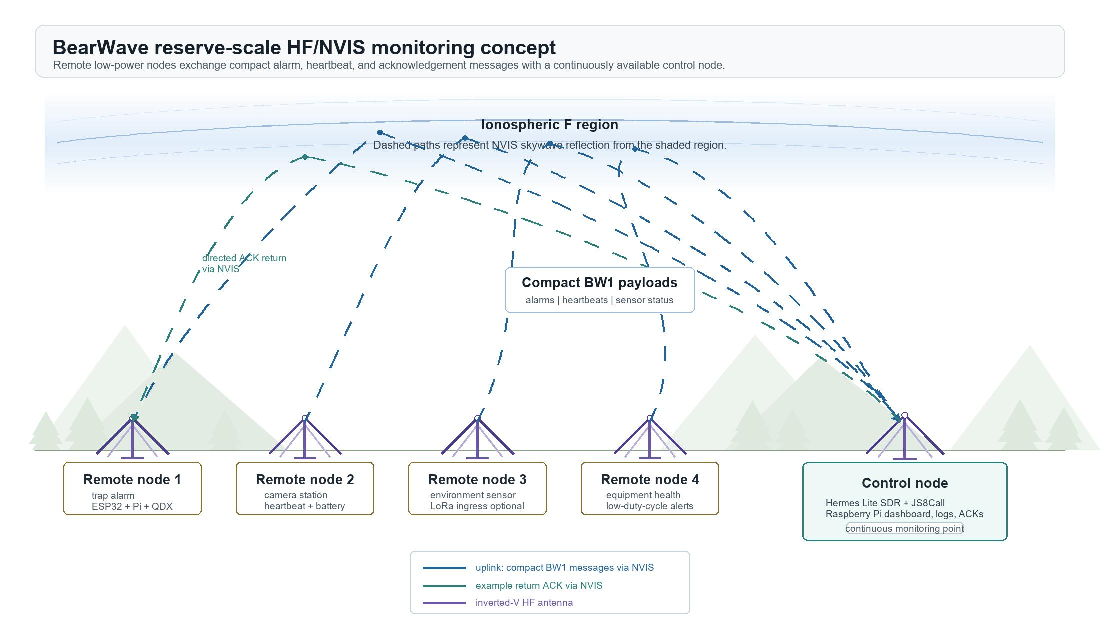
\includegraphics[width=1.08\linewidth]{images/bearwave_nvis_network_overview.pdf}}
    \caption{Network-level BearWave monitoring concept showing four remote trap and sensor nodes communicating with a continuously available control node using HF/NVIS skywave paths and inverted-V dipole antennas. Remote nodes remain in low-power supervision for most of their duty cycle and wake to transmit compact BearWave messages; directed acknowledgements return through the same NVIS mechanism. When an alarm is acknowledged, the current implementation can also transmit a linked SSTV still image before shutdown.}
    \Description{Conceptual network diagram showing four remote BearWave nodes deployed across a reserve. Each remote node has an inverted-V dipole antenna and sends a dashed HF/NVIS skywave path that reflects from a shaded ionospheric F region before reaching a fixed control node with its own inverted-V dipole. A representative directed acknowledgement path is also shown returning by NVIS reflection. The control node contains a Hermes Lite SDR, JS8Call, Raspberry Pi dashboard, logs, and acknowledgement function.}
    \label{fig:nvis-network-overview}
\end{figure}

The paper is therefore framed as a system design and open hardware report rather than a second propagation study. Its closest publication model is the AudioMoth hardware paper, which made a conservation technology valuable by documenting not only what it did, but how it could be built, configured, validated, and deployed \cite{Hill2019AudioMothHardware}. BearWave requires the same treatment: the control node, remote node hardware, ESP32 supervisory firmware, Raspberry Pi software, message format, and validation workflow must be described as a coherent reusable system.

The final BearWave design emerged from a practical limitation in early Raspberry Pi-centred prototypes. A Pi is attractive because it can run mature radio software, file logging, and higher-level control code, but it is poorly matched to continuous unattended sensing when power is limited. Keeping Linux, audio/radio interfaces, and application logic awake merely to watch for occasional trap or status events would waste energy and shorten field life. The revised architecture therefore separates continuous supervision from intermittent communication. A Heltec ESP32 remains responsible for the low-power tasks that must always be available, while the Raspberry Pi and radio chain are treated as a higher-power subsystem that is only energised during a communication cycle. This efficiency goal is both electrical and practical: lower quiescent power extends battery life and reduces maintenance visits, while low-cost, field-serviceable components make the system more realistic for conservation organisations to build, repair, and scale.

This separation also changes the contribution of the paper. The earlier BearWave work asked whether a low-power HF/NVIS link could provide useful communication under difficult non-line-of-sight conditions. This paper asks how that link can be embedded into a complete system that a conservation team can build and maintain. The resulting design combines an ESP32 supervisory layer, a Raspberry Pi communication layer, a QRP Labs QDX and modified ATU100 RF chain, an inverted-V dipole arrangement, a Hermes Lite SDR control node, and a compact application-layer message format. The research contribution is therefore the integration and documentation of a complete open system rather than a single isolated subsystem.

\subsection{Research Questions and Scope}
\begin{enumerate}[label=\textbf{RQ\arabic*.}]
    \item How can BearWave be structured as an open, reproducible conservation monitoring system rather than a single communication prototype?
    \item How do the control node, remote node hardware, ESP32 supervisory firmware, Raspberry Pi software, message format, and SSTV extension interact to convert local field events into long-haul HF/NVIS alerts with optional visual context?
    \item What validation steps are required to demonstrate that a locally built BearWave unit is electrically, functionally, and operationally ready for field deployment?
    \item What design limitations remain before long-term rainforest deployment, particularly around enclosure, energy autonomy, and large-scale multi-node operation?
\end{enumerate}

\subsection{Contributions}
\begin{enumerate}[label=\textbf{C\arabic*.}]
    \item A complete system architecture for BearWave, separating the control node, remote node hardware, ESP32 supervisory firmware, Raspberry Pi communication software, and message protocol.
    \item A documented remote node hardware design integrating sensing inputs, timing support, battery monitoring, protected power input, and switchable 5 V and 12 V rails.
    \item A reproducible software and message-flow description showing how trap, heartbeat, and sensor events are normalised, queued, transmitted, logged, acknowledged, and, for alarm events, optionally followed by a linked SSTV still image.
    \item A validation and deployment workflow intended to let conservation organisations build and test BearWave nodes without specialist laboratory infrastructure.
\end{enumerate}

To make this contribution explicit in the same spirit as open hardware reports such as AudioMoth, Table~\ref{tab:hardware-summary} summarises BearWave as a reproducible conservation technology rather than as a single experimental radio link.

\begin{table}[H]
\centering
\caption{BearWave reproducibility and hardware summary.}
\label{tab:hardware-summary}
\begin{tabularx}{\textwidth}{p{0.28\textwidth}X}
\toprule
Attribute & BearWave description \\
\midrule
System name & BearWave \\
Subject area & Conservation technology, remote sensing, open ecological hardware, low-power field monitoring \\
Hardware type & Low-bandwidth trap, sensor, and equipment-health monitoring system with remote field nodes and a fixed control node \\
Primary field constraint & Remote conservation sites without reliable mains power, cellular coverage, terrestrial backhaul, or affordable satellite telemetry \\
Remote-node platform & Heltec ESP32 supervisor, Raspberry Pi Zero 2 W communication layer, QRP Labs QDX, modified ATU100, GPS/RTC timing support, battery monitoring, switched rails, sensor inputs, and camera/SSTV capture extension \\
Control-node platform & Raspberry Pi 4, touchscreen kiosk dashboard, Hermes Lite SDR, SparkSDR, JS8Call, QSSTV receiver, Node.js service, local logging, and acknowledgement scheduler \\
Communication method & Compact BearWave application messages carried over low-power HF/NVIS digital-mode transmissions, with optional alarm-triggered PD240 SSTV still-image transmission as a secondary path \\
Open artefacts & PCB files, schematic, bill-of-materials information, firmware, Raspberry Pi scripts, SSTV capture/encode/transmit scripts, control-node software, message-format documentation, configuration examples, and validation workflow \\
Intended deployment scale & Small reserve-scale deployments, approximately ten trap or sensor monitoring points per control node in the present design \\
System maturity & Integrated hardware/software research prototype with bench and controlled-field validation workflow; enclosure, security, and long-duration rainforest deployment remain future work \\
\bottomrule
\end{tabularx}
\end{table}

\section{Related Work and System Positioning}
\subsection{Remote Conservation Monitoring}
Remote conservation monitoring is shaped by a mismatch between ecological need and infrastructure availability. Traps, camera stations, acoustic devices, water-level sensors, and security monitors are often deployed in places where staff access is slow, expensive, or risky. In tropical forest sites, daily inspection can be constrained by flooding, vegetation, terrain, wildlife, and limited vehicle or boat access \cite{ButterworthMarkAndrew2025ERCi}. These constraints are not merely logistical: delayed trap inspection can become an animal-welfare issue, while delayed detection of equipment failure can undermine long-term research datasets.

The first two BearWave papers established this conservation setting and the communication problem that follows from it. Dense vegetation and non-line-of-sight terrain limit many short-range radio systems, while cellular coverage is often absent and satellite options may be too costly or power intensive for large numbers of simple monitoring points. The system described here is positioned as a low-bandwidth field infrastructure component: it is intended to carry small but operationally important messages such as trap alarms, low-battery warnings, heartbeats, and equipment-health reports.

\subsection{Communication Options for Dense and Remote Habitats}
Several communication approaches are available for remote monitoring, but each carries a different assumption about infrastructure, power, range, and message volume. Wi-Fi and cellular systems work well where supporting infrastructure already exists, but they are poorly matched to isolated forest sites without backhaul. LoRa and LoRaWAN can be highly effective for low-power sensing, yet their range and reliability are strongly shaped by terrain, antenna height, gateway placement, and vegetation. Satellite IoT and satellite messengers reduce dependence on local infrastructure, but they introduce subscription costs, power demands, sky-view requirements, and device-level constraints. HF/NVIS communication occupies a different design point: it is narrowband and operationally more specialised, but it can provide long-haul communication without terrestrial relay infrastructure.

\begin{table}[H]
\caption{Positioning of BearWave relative to common communication options for remote conservation monitoring.}
\label{tab:communication-options}
\begin{tabularx}{\linewidth}{p{0.20\linewidth}p{0.27\linewidth}X}
\toprule
Option & Strength & Limitation for the BearWave use case \\
\midrule
Wi-Fi or cellular & Mature, high throughput, familiar tooling & Requires local infrastructure or coverage that may be absent in remote reserves. \\
LoRa/LoRaWAN & Low power and well suited to local sensor networks & Gateway placement, terrain, vegetation, and link budget may limit long-haul coverage. \\
Satellite IoT & Independent of terrestrial network infrastructure & Higher cost, power, subscription, and sky-view constraints can limit dense deployment. \\
Commercial trap monitors & Purpose-built and often operationally polished & Can be expensive, closed, difficult to repair locally, and hard to adapt to new sensors. \\
HF/NVIS & Long-haul low-bandwidth communication without terrestrial relay infrastructure & Requires careful antenna deployment, frequency choice, regulatory compliance, and protocol discipline. \\
\bottomrule
\end{tabularx}
\end{table}

BearWave does not claim to replace every other approach. Instead, it targets the gap where messages are small, infrastructure is absent, and local organisations need a system they can adapt without dependence on proprietary service chains. LoRa remains useful for local ingress and satellite remains valuable where cost and power are acceptable; BearWave provides a complementary route for sparse but important long-haul alerts.

\subsection{Open Ecological Hardware}
Open ecological hardware has become important because conservation technology must often be repaired, modified, and understood far from the laboratory that produced it. A design is not truly reusable simply because a schematic or source file exists. For practical adoption, users need a bill of materials, assembly notes, configuration steps, validation procedures, example operating modes, and a frank account of limitations. The AudioMoth paper is a useful model because it presents the device as a reproducible platform rather than as an opaque instrument \cite{Hill2019AudioMothHardware}.

BearWave follows the same reporting logic. The system contains several coupled components: a control node, field hardware, supervisory firmware, Pi-side software, radio equipment, antenna deployment, and a message protocol. A weakness in any one of these can prevent the system from working in the field. The paper therefore documents not only the final behaviour but also the build and validation path needed to reproduce that behaviour.

\subsection{Gap Addressed by This Paper}
The gap addressed by this paper is the transition from a validated communication idea to a buildable conservation monitoring system. Earlier BearWave work established the conservation need, demonstrated low-power HF/NVIS feasibility in temperate woodland, and then evaluated the approach under Borneo rainforest conditions \cite{ButterworthMarkAndrew2025ERCi,Butterworth2026BorneoFieldTrial}. What remained missing was the surrounding system: how a remote node detects and preserves events, how it wakes the Pi and radio chain, how the message is encoded, how the control node reconstructs and acknowledges messages, how the design is assembled, and how a completed unit is validated before deployment.

This paper therefore positions BearWave as open infrastructure for remote conservation monitoring. Its novelty lies in the integration of low-power hardware supervision, intermittent Linux-based radio control, compact HF messaging, and a reproducible build workflow. This is the system layer required before the communications result can be adopted by other conservation groups.

\section{System Requirements and Design Objectives}
The system requirements follow directly from the intended operating environment. A BearWave node must sit at the edge of a conservation site, observe simple physical or sensor events, and report them without assuming mains power, cellular coverage, or frequent human access. The control node must remain continuously available and operator-facing, while the remote node must minimise active energy use and tolerate intermittent communication success. The design is also constrained by cost: the system avoids unnecessary specialist equipment, subscriptions, and proprietary dependencies so that multiple nodes can be built and maintained within realistic conservation budgets.

\subsection{Operational Requirements}
\begin{itemize}
    \item Monitor traps, camera stations, and simple environmental sensors without requiring daily physical visits.
    \item Support both directly wired trigger inputs and local LoRa sensor ingress so that additional measurements can be added without changing the remote-node PCB.
    \item Report alarms and periodic heartbeat/status messages to a central point without terrestrial communications infrastructure.
    \item Minimise baseline current draw so that high-power compute and RF subsystems are active only when required.
    \item Maximise battery life and service interval so that field staff are not required to visit remote nodes simply to maintain power.
    \item Use low-cost, field-serviceable components where possible so that the system can be replicated, repaired, and scaled by conservation users.
    \item Support multi-node deployments while keeping the intended operational scale manageable for field staff, with the present design aimed at approximately ten trap-monitoring points per control node.
    \item Be reproducible from documented hardware files, software repositories, and bill-of-materials information.
    \item Provide deployment procedures suitable for conservation staff and collaborating researchers.
\end{itemize}

\subsection{Design Principles}
\begin{table}[tbp]
\centering
\caption{Design principles used to organise BearWave as reusable system building blocks.}
\label{tab:design-principles}
\begin{tabularx}{\textwidth}{p{0.28\textwidth}X}
\toprule
Principle & Consequence for the paper \\
\midrule
Describe the system by node role & Separate control-node design from remote-node design so each can be built and evaluated independently. \\
Design for energy and cost efficiency & Treat low quiescent power, short high-load duty cycles, affordable parts, and realistic service intervals as primary system requirements rather than later optimisations. \\
Separate hardware from firmware behaviour & Present the remote PCB, switched rails, sensors, and timing hardware before describing ESP32 and Raspberry Pi software. \\
Treat the message format as a first-class interface & Document payload fields, message classes, timing, acknowledgements, and error handling in a dedicated section. \\
Allow flexible local sensing & Support nearby LoRa-connected sensors, such as temperature, humidity, and equipment-health devices, so that a remote node can accept additional local measurements without hardware redesign. \\
Follow open-hardware reporting practice & Include design files, bill of materials, assembly guidance, validation tests, and deployment procedures. \\
Keep evaluation aligned with system claims & Characterise power, latency, trigger reliability, message delivery, and field serviceability rather than only RF propagation. \\
Separate theoretical capacity from operational scale & Report that the protocol and control node can represent many remote nodes, while making clear that the practical design target is a small, manageable deployment rather than a maximum-density network. \\
\bottomrule
\end{tabularx}
\end{table}

\section{Overall BearWave System Design}
BearWave is designed as a complete low-bandwidth monitoring system rather than as a single radio experiment. The system combines field sensing, low-power supervision, switched compute, HF digital communication, a compact application-layer protocol, and an operator-facing control node. A central requirement is that normal operation is fully automated: once a remote node and control node are configured and running, the system observes events, wakes and shuts down the remote communication hardware, transmits heartbeats or alarms, processes acknowledgements, logs messages, and updates the dashboard without routine user input. Human attention is therefore intended to be exception-based, primarily when an alarm, missed heartbeat, low-battery condition, or maintenance state is presented by the control node.

The central design problem is asymmetry: the remote node must conserve energy and survive unattended field use, while the control node can remain powered, listening, logging, and visible to an operator. The architecture therefore gives each node a different role, rather than attempting to run the same software and hardware at both ends of the link.

\subsection{Network Topology and Node Roles}
BearWave is organised around two principal node types. The remote node is the field-deployed monitoring unit. It is responsible for observing local sensors, preserving event state, waking higher-power subsystems only when necessary, transmitting compact HF/NVIS messages, waiting for acknowledgements where supported, and returning to a low-power state. In addition to directly wired inputs, each remote node can act as a local collection point for nearby low-power LoRa sensors. This allows measurements such as temperature, humidity, contact state, or equipment-health indicators to be added through firmware and message-format extensions rather than through a new PCB revision. The control node is the fixed receiving and management point. It listens continuously for BearWave messages, reconstructs and validates payloads, logs received events, derives node-health state, presents alarms to the operator, and schedules acknowledgements back to the remote node. This division allows the operator interface to act primarily as a supervisory display and alerting point, rather than as a console that must be actively managed during routine monitoring.

The remote node is built around a layered hardware model. A Heltec ESP32 module acts as the low-power supervisor and remains responsible for trap inputs, battery state, GPS/RTC time context, event latching, and power-rail control. A Raspberry Pi Zero 2 W provides the Linux-based application and radio-control layer. It is powered only during communication windows, when it queries the ESP32, constructs a BearWave message, controls the JS8Call transmission process, and manages acknowledgement handling. The HF radio subsystem consists of a QRP Labs QDX digital transceiver, a modified ATU100 automatic antenna tuner, and an inverted-V dipole antenna arrangement. The ATU100 has been adapted for operation below the power level normally required by the standard design, allowing the remote node to tune and operate in the sub-10 W QRP range required by the power budget.

The control node uses a Raspberry Pi 4 with a touch display as the operator-facing computer. Its radio interface is a Hermes Lite SDR, used with JS8Call as the HF digital-mode endpoint for continuous receive and directed acknowledgement transmission. The control-node application is deliberately kept separate from the radio transport: JS8Call and the Hermes Lite SDR provide the RF and digital-mode path, while the BearWave software performs fragment assembly, protocol parsing, node-state management, acknowledgement scheduling, logging, and dashboard presentation.
For alarm verification the same base-station audio path is also made available to an SSTV receiver. In the tested configuration SparkSDR provides the Hermes Lite receive audio, JS8Call decodes BearWave text messages, and QSSTV listens in parallel for SSTV images. This preserves the text-first BearWave alarm path while allowing a received image to be displayed beside the node that raised the alarm. The alarm message is the operationally important part of the system: it is the low-power, acknowledged message that establishes the event record and drives the conservation response. The image path is deliberately best-effort, providing useful visual context when it decodes successfully but not forming a guaranteed part of alarm delivery.
The reproducibility record treats the RF installation as part of the system rather than as a background condition. It records the Hermes Lite revision, operating band, dipole dimensions, feed-point arrangement, support height, power source, acknowledgement-transmit arrangement, and ATU100 low-power modification because these practical details determine whether another group can reproduce the same radio chain.

\begin{figure}[tbp]
    \centering
    \makebox[\linewidth][c]{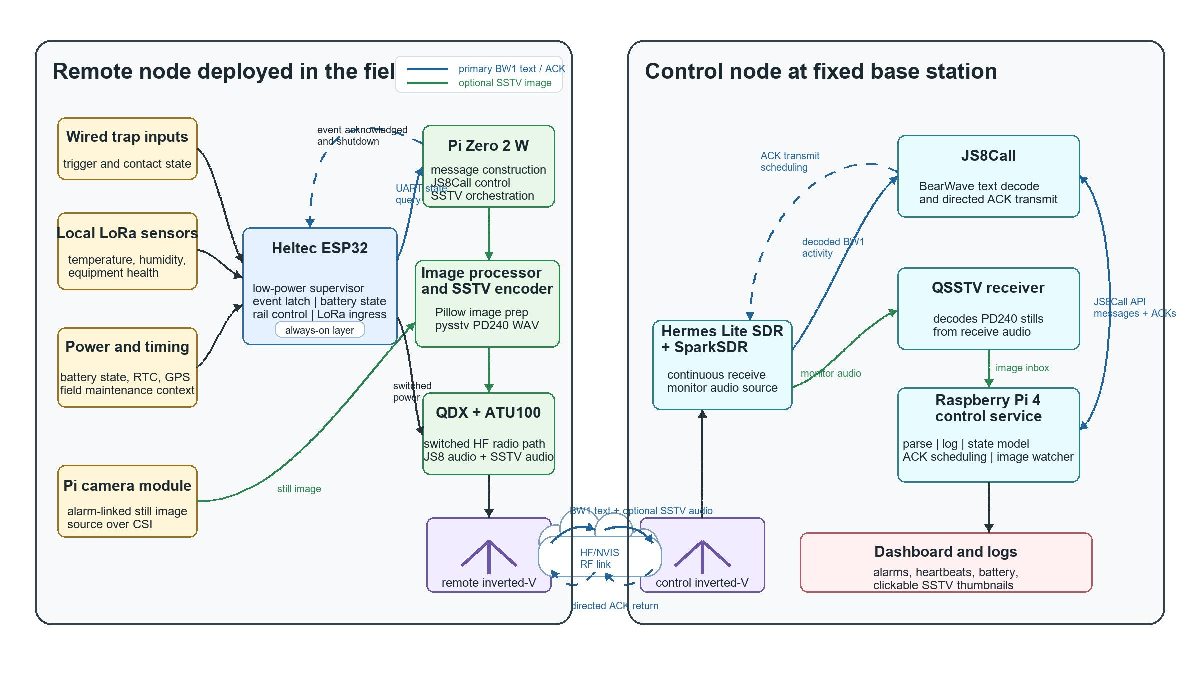
\includegraphics[width=1.15\linewidth]{images/bearwave_system_architecture.pdf}}
    \caption{BearWave system architecture showing the remote-node sensing and power-management path, the switched Raspberry Pi and QDX/ATU100 HF transmission path, the primary BearWave text and acknowledgement path, and the optional best-effort SSTV image path from camera capture to control-node thumbnail display.}
    \Description{System architecture diagram with a field remote node on the left and a fixed control node on the right. Wired trap inputs, LoRa sensors, battery, RTC, and GPS feed the ESP32 supervisor. The ESP32 wakes a Raspberry Pi Zero 2 W and QDX/ATU100 radio path for compact JS8Call and BW1 text transmission over HF/NVIS. A separate camera branch feeds Pi-side image preparation and PD240 SSTV encoding, which uses the same radio/audio path after an acknowledged alarm. At the control node, Hermes Lite SDR and SparkSDR feed JS8Call for text reception and acknowledgements, and QSSTV for SSTV image reception. The Raspberry Pi 4 control service logs events, manages acknowledgements and the image watcher, and presents alarms, status, and clickable SSTV thumbnails on the dashboard.}
    \label{fig:functional-architecture}
\end{figure}

\begin{table}[tbp]
\caption{Principal BearWave system blocks and their architectural roles.}
\label{tab:system-blocks}
\begin{tabularx}{\linewidth}{p{0.24\linewidth}X}
\toprule
System block & Role in the complete system \\
\midrule
Local sensors and trap inputs & Provide the physical event source, including trap triggers, battery state, and environmental or equipment-health sensors connected directly or through local LoRa ingress. \\
ESP32 supervisor & Maintains low-power field supervision, latches events, controls switched rails, exposes state over UART, and removes power from the Pi/radio subsystem after shutdown. \\
Raspberry Pi Zero 2 W & Runs the remote-node application logic, builds BearWave messages, interacts with JS8Call, handles acknowledgements, and persists failed critical messages. \\
QRP Labs QDX & Provides the remote-node HF digital transceiver path used for low-power JS8Call/BearWave message transmission and, during the SSTV extension stage, audio playback of the generated SSTV waveform. \\
Modified ATU100 & Matches the field antenna to the QDX at QRP power levels, enabling practical remote deployment with less than 10 W available for tuning and transmission. \\
Inverted-V dipole & Provides the HF/NVIS antenna arrangement used by the BearWave radio link. The deployment record includes band, wire length, feed-point height, end height, feedline, choke or balun arrangement, and mounting method. \\
Hermes Lite SDR & Provides the control-node HF SDR interface for continuous reception and, where enabled, acknowledgement transmission. \\
Control-node software & Reconstructs fragmented JS8Call activity, validates BearWave payloads, updates node state, logs events, schedules acknowledgements, watches the SSTV image inbox, and serves the operator dashboard. \\
\bottomrule
\end{tabularx}
\end{table}

\subsection{End-to-End Data Path}
The end-to-end data path begins at the field sensor rather than at the radio. A trap trigger, low-battery condition, scheduled heartbeat, or other local event is first observed by the ESP32 supervisor. The ESP32 validates and latches the event so that a short physical trigger is not lost while the Raspberry Pi is powered down. If communication is required, the ESP32 enables the 5 V rail that powers the Raspberry Pi and the 12 V rail that supplies the radio/tuner subsystem. The Pi boots into its communication cycle, opens the UART link to the ESP32, and requests the current time, battery state, coordinates where available, and event summary.

The Pi then constructs a compact BearWave application-layer payload. Routine status is normally transmitted as a heartbeat, while non-critical environmental telemetry can be carried as a sensor-report payload, for example humidity, temperature, or other locally attached sensor values. Trap and low-battery conditions are transmitted as critical messages and are eligible for persistence if no acknowledgement is received. The message is handed to JS8Call for transmission through the QDX and the tuned inverted-V dipole antenna path provided by the modified ATU100. The RF path is intended for low-power HF/NVIS operation, allowing a field node to reach a fixed base station without reliance on cellular coverage, satellite subscriptions, or reserve-wide terrestrial infrastructure.

At the control node, the Hermes Lite SDR and JS8Call receive the on-air signal and expose decoded activity through the JS8Call TCP API. JS8Call receive activity may arrive as fragments, so the control-node software reconstructs complete BearWave frames before validation. Once a valid message is decoded, the control node updates its in-memory node-state model, records raw and structured log entries, refreshes the browser dashboard, and raises any operator alarm state. If acknowledgement is enabled, the control node schedules a compact directed acknowledgement after a configured delay. This delay allows the remote node to complete its own transmit sequence and enter the receive window in which it can hear the reply. The acknowledgement is then handed back to JS8Call and transmitted through the control-node radio path.

When the message is an alarm and the SSTV extension is enabled, the acknowledged text alert is followed by a separate still-image transmission. The image is not embedded in the \texttt{BW1} payload. Instead, the control node treats the decoded alarm as the primary event record and waits for a subsequently received SSTV image in the local image inbox. The dashboard then presents the still image as a clickable thumbnail on the corresponding node card. This keeps the alarm channel compact and robust while providing visual context when channel quality and power budget allow the longer image transmission. If no image is received, the alarm is still valid and actionable because the acknowledged compact message has already completed the reliable low-power reporting function.

When the remote Pi receives a matching acknowledgement, it reports successful delivery back to the ESP32 using the UART event-acknowledgement command. The ESP32 can then suppress repeated presentation of that same event until the underlying physical condition clears and re-arms. Finally, the Pi requests shutdown and the ESP32 removes power from the Pi/radio rail after the configured Linux shutdown delay. This closes the cycle by returning the remote node to low-power supervision while leaving the control node continuously available for the next message.

\subsection{Operating Modes}
BearWave behaviour can be described as a small set of operating modes. These modes are distributed across the two node types: the remote node moves between low-power supervision and short communication windows, while the control node remains in a persistent monitoring mode.

\begin{table}[tbp]
\caption{BearWave operating modes and dominant system responsibilities.}
\label{tab:system-operating-modes}
\begin{tabularx}{\linewidth}{p{0.24\linewidth}X}
\toprule
Mode & Behaviour \\
\midrule
Idle supervision & The ESP32 remains active at low power, monitors trap inputs and battery state, keeps time context, and holds the Pi/radio subsystem off. \\
Event latch & A trap or low-battery condition is latched by the ESP32 so the event remains available to the Pi even if the physical trigger is brief. \\
Scheduled heartbeat & At a configured interval, the ESP32 wakes the Pi so a routine status message can be transmitted. \\
Pi wake and state acquisition & The Pi boots, confirms the ESP32 is alive, reads time, battery, coordinates, and event state, then decides whether to send a heartbeat or critical alarm. \\
HF message transmission & The Pi hands a compact BearWave payload to JS8Call for transmission through the QDX and tuned inverted-V dipole antenna path. \\
SSTV image transmission & For acknowledged alarm cycles, the Pi can capture an image, encode it as an SSTV audio waveform, and transmit it through the same QDX audio path before shutdown. \\
Acknowledgement wait & The Pi listens for a matching acknowledgement from the control node. The control node delays and duplicate-suppresses acknowledgements to fit the remote receive window. \\
Retry and persistence & Failed critical messages are stored locally for retransmission on the next boot; failed routine heartbeats are not persisted. \\
Managed shutdown & The Pi reports delivery outcome, requests shutdown, and the ESP32 removes rail power after the configured delay. \\
Control-node monitoring & The Raspberry Pi 4, Hermes Lite SDR, JS8Call, Node.js service, and dashboard remain continuously available for receive, logging, alarm presentation, and acknowledgement transmission. \\
Image receive and display & QSSTV listens to the control-node receive audio path, writes decoded still images into the BearWave image inbox, and the dashboard presents the latest image as a clickable node thumbnail. \\
Maintenance & Local service access allows firmware flashing, configuration changes, radio/tuner checks, dashboard inspection, and log recovery. \\
\bottomrule
\end{tabularx}
\end{table}

\subsection{System Interfaces}
The system boundary is defined by a set of deliberately simple interfaces. At the edge of the remote node are physical sensor inputs, battery measurement, GPS/RTC timing, switched power rails, and the HF antenna system. Inside the remote node, the ESP32-to-Pi UART forms the key local software boundary: the Pi does not need to know raw GPIO state or rail-control details, and the ESP32 does not need to implement JS8Call or BearWave message construction. Across the RF link, the BearWave application-layer message is the stable interface. At the control node, JS8Call exposes decoded activity and transmit commands through its TCP API, while the Node.js service exposes operator state through HTTP, WebSocket updates, and persistent logs.

\begin{table}[tbp]
\caption{Major BearWave system interfaces.}
\label{tab:system-interfaces}
\begin{tabularx}{\linewidth}{p{0.24\linewidth}X}
\toprule
Interface & Purpose \\
\midrule
Trap and sensor inputs & Connect physical conservation events and environmental sensors to the ESP32 supervisor. \\
Battery and rail sensing & Allows the supervisor and Pi software to report supply state, detect low battery, and verify switched-rail behaviour. \\
GPS and RTC & Provide location and time context for local logs, message construction, wake scheduling, and later event interpretation. \\
ESP32-Pi UART & Carries simple textual commands for time, battery, coordinates, event state, event acknowledgement, and shutdown. \\
Pi-JS8Call API & Allows the remote Pi application to transmit BearWave payloads and wait for directed acknowledgements. \\
Camera and SSTV encode path & Allows the remote Pi to capture an alarm-linked still image, prepare it with local image-processing software, and encode it as a PD240 SSTV audio waveform. \\
QDX/ATU100 path & Provides the remote-node low-power HF transmit path from digital-mode software to the tuned inverted-V dipole. \\
Hermes Lite/JS8Call path & Provides the control-node HF receive and acknowledgement-transmit path for compact BearWave messages. \\
Hermes Lite/QSSTV path & Provides the parallel control-node SSTV receive path used to decode alarm-linked still images. \\
BearWave protocol & Defines the compact over-the-air grammar shared by remote and control nodes. \\
Dashboard and logs & Convert decoded messages into operator-visible status, alarms, acknowledgement records, and research data for later analysis. \\
\bottomrule
\end{tabularx}
\end{table}

This overview provides the organising structure for the rest of the paper. The following sections describe each building block in more detail: the control node as the persistent base station, the remote-node hardware as a low-power field platform, the ESP32 and Raspberry Pi software as cooperating control layers, and the BearWave message protocol as the compact interface that allows the system to operate over a constrained HF/NVIS link.

\section{Control Node Design}

\subsection{Control Node Role}
The BearWave control node is the continuously available base-station component of the system. Its role is not simply to receive text from JS8Call, but to convert intermittent, fragmented radio activity into an operator-facing model of remote-node health. It maintains the latest known state of each remote node, records valid BearWave messages, raises local alarms, schedules acknowledgements, and presents the resulting network status on a touchscreen dashboard. In the present implementation it is best understood as a prototype supervisory monitor rather than a complete production command system, but the software structure is intentionally modular so that additional command, export, or cloud-integration functions can be added without changing the BearWave message grammar.

This division is important because BearWave uses asymmetric duty cycles. The remote node is designed to spend most of its time in a low-power supervised state and to activate the Raspberry Pi and radio path only for a bounded communication window. The control node has no equivalent power constraint and can therefore remain ready to receive, reconstruct, timestamp, and acknowledge messages at all times. The control node also provides the place where richer diagnostic information can be stored without increasing the over-the-air payload. Received JS8Call metadata, message-assembly events, acknowledgement timing, and operator actions can all be logged locally while the radio message itself remains compact.

\subsection{Control Node Hardware}
The present control-node implementation uses a Raspberry Pi 4 with an attached touch display. This gives the control node enough processing capacity to run JS8Call, the Node.js supervisory service, a local web server, Socket.IO updates, and a browser-based dashboard in a kiosk-style arrangement. The design assumes that the control node remains powered and physically accessible to an operator, which allows it to prioritise availability and observability rather than extreme power saving.

\begin{figure}[tbp]
    \centering
    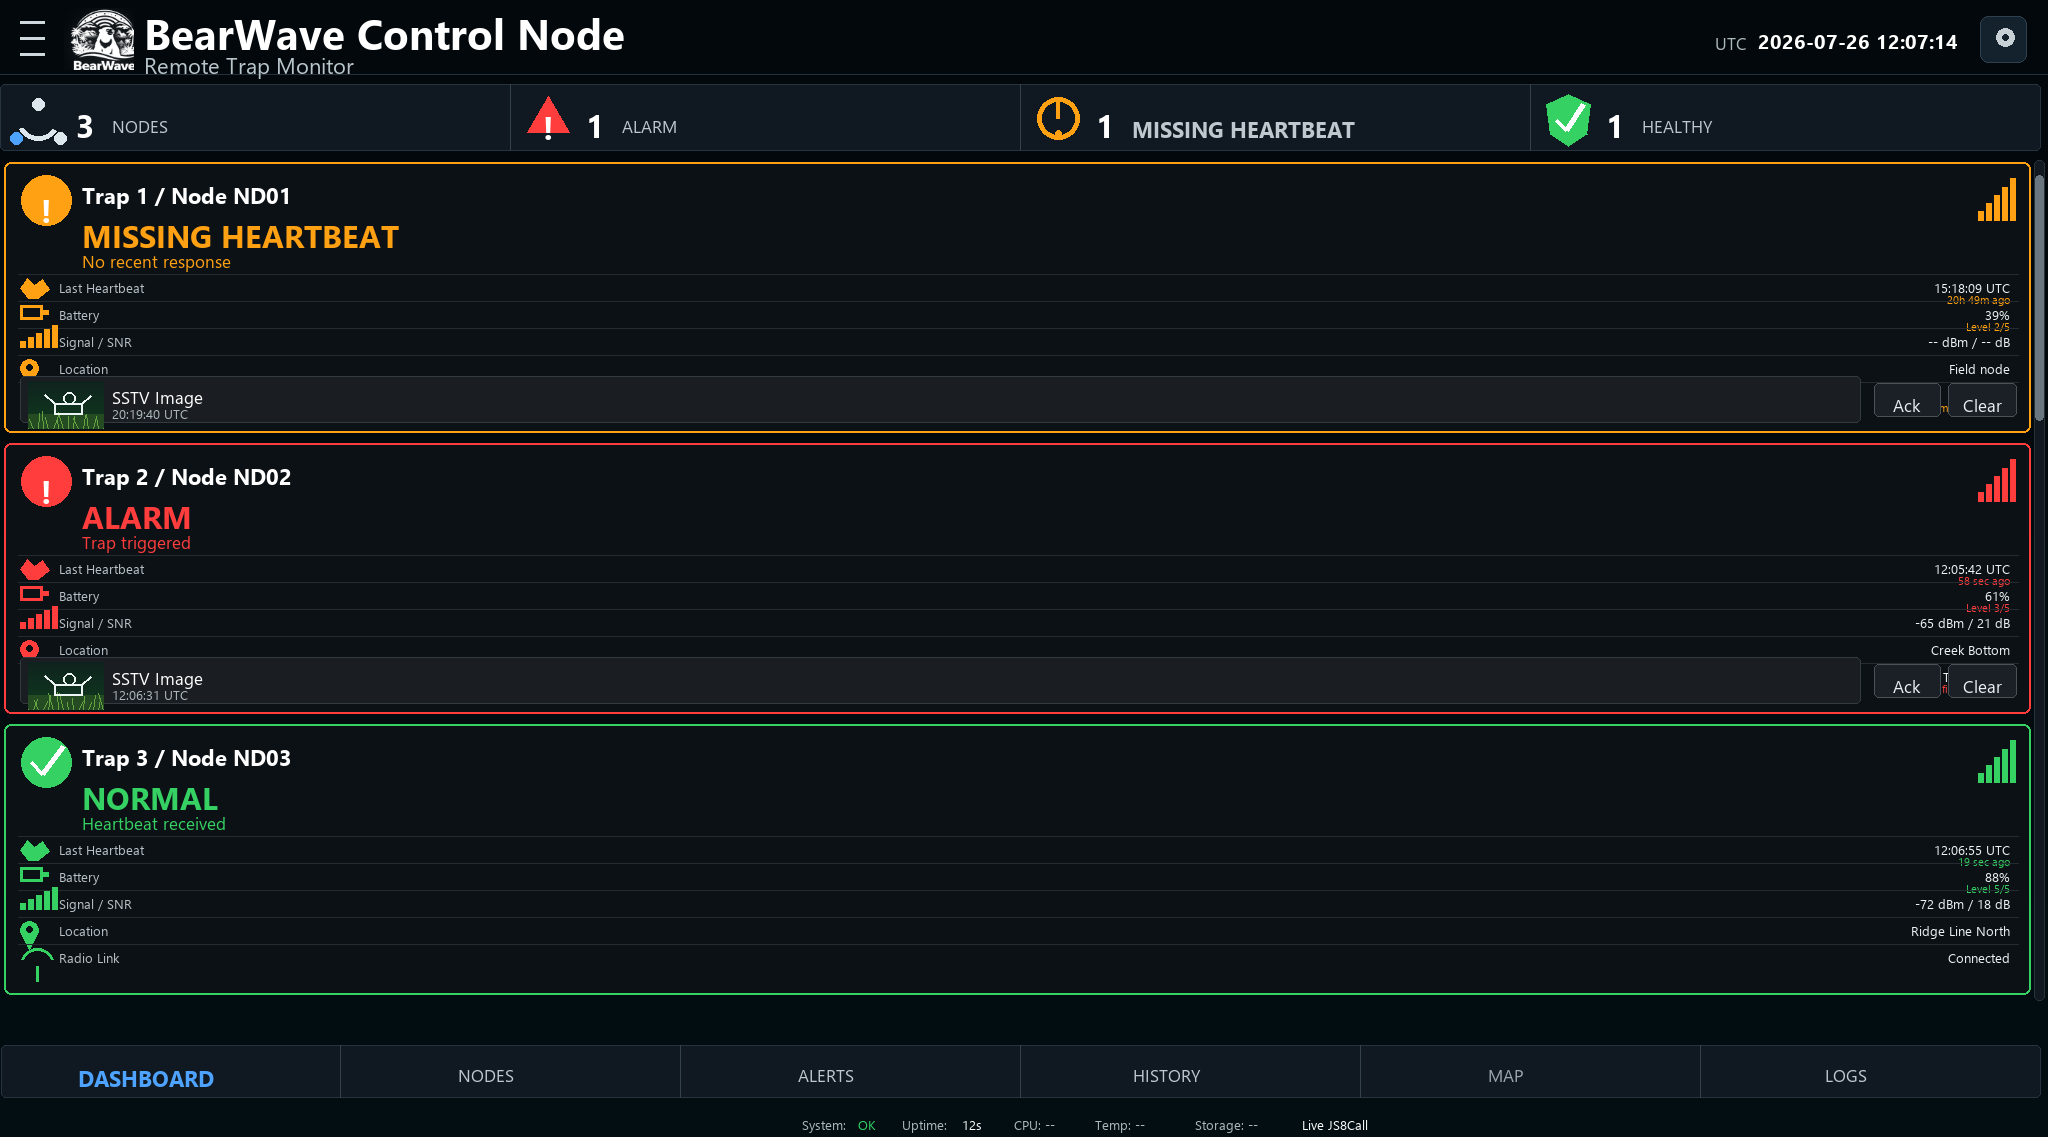
\includegraphics[width=0.95\linewidth]{images/control_node_dashboard.png}
    \caption{BearWave control-node dashboard concept based on the current list-style operator display, showing three connected remote trap nodes in different states: one missing-heartbeat node, one alarmed node, and one healthy node. Received SSTV images are presented as clickable thumbnail rows within the relevant node panel.}
    \Description{Live-style control-node dashboard display with a top summary bar, three vertically stacked trap panels, a right-hand scroll bar, bottom navigation, and system status strip. Trap 1 is shown with a missing-heartbeat warning and an SSTV image row, Trap 2 is shown in alarm with a triggered trap state and an SSTV image row, and Trap 3 is shown as normal and healthy. Each panel includes heartbeat, battery, signal, location, and radio-link or trap-status information.}
    \label{fig:control-node-dashboard}
\end{figure}

\begin{table}[tbp]
\caption{Control-node components and documented responsibilities in the current prototype.}
\label{tab:control-node-components}
\begin{tabularx}{\linewidth}{p{0.24\linewidth}X}
\toprule
Component & Function in the BearWave control node \\
\midrule
Raspberry Pi 4 & Hosts the Node.js supervisory service, local HTTP service, Socket.IO updates, dashboard files, and control-node logs. \\
Touch display & Provides a local operator interface for node health, alarms, received images, event history, and logs. \\
JS8Call instance & Provides the HF digital-mode transport interface and exposes received and transmitted events through its local TCP API. \\
SparkSDR and QSSTV & Provide the practical receive chain for SSTV image decoding, with SparkSDR supplying the receive audio and QSSTV writing decoded images to the local BearWave image inbox. \\
Hermes Lite SDR & Provides the base-station SDR hardware used for continuous HF receive and, where enabled, acknowledgement transmission. \\
Inverted-V dipole & Provides the base-station HF/NVIS antenna arrangement for the Hermes Lite SDR path. The deployment record states the dimensions, feedline, support height, and operating band. \\
Local storage & Stores line-delimited raw JS8Call events and structured BearWave event logs for later timing analysis. \\
\bottomrule
\end{tabularx}
\end{table}

\subsubsection{Hermes Lite SDR and Base-Station RF Path}
The Hermes Lite SDR forms the control node's HF radio front end. In the BearWave architecture it is not used as a general-purpose experimentation receiver, but as the fixed base-station radio interface for a continuously running monitoring node. Its primary role is to keep the control node listening for low-power JS8Call traffic from remote nodes. Where acknowledgements are enabled, the same base-station RF path also supports directed return messages from the control node to the originating remote node.

This arrangement complements the remote-node design. The remote node uses a QDX, modified ATU100, and inverted-V dipole during short communication windows; the control node uses the Hermes Lite SDR and its own inverted-V dipole as the always-available counterpart. This asymmetry is intentional. The remote node is energy-limited and spends most of its time with the Pi/radio subsystem powered down, while the control node is installed where continuous power, local operator access, and persistent logging are practical.

The control node treats the Hermes Lite SDR, SparkSDR, JS8Call, and QSSTV as transport and decode tools. Radio tuning, receive audio, transmit audio, transmit/receive control, and SSTV demodulation belong to this radio-software setup, while BearWave-specific logic remains in the Node.js application. This separation is important for reproducibility: a future implementation could change the SDR-control program, SSTV receiver, or radio hardware without changing the BearWave message format, node-state model, acknowledgement scheduler, or image-inbox interface.

\begin{table}[tbp]
\caption{Control-node Hermes Lite SDR setup and documentation requirements.}
\label{tab:control-node-hermes-lite-setup}
\begin{tabularx}{\linewidth}{p{0.26\linewidth}X}
\toprule
Setup element & Required description for the paper \\
\midrule
Hermes Lite SDR & State the exact hardware revision, firmware version if relevant, RF connection, operating band, and whether the SDR is used for both receive and acknowledgement transmission. \\
SDR-to-Pi connection & Document how the Raspberry Pi 4 communicates with the SDR and how the SDR-control application is started, including Ethernet, SDR software, rig-control bridge, audio path, or other integration details used in the final build. \\
JS8Call integration & Describe how JS8Call receives decoded audio from the SDR path and how outgoing directed acknowledgements are handed back for transmission, including audio routing, CAT/PTT, frequency control, and startup order. \\
QSSTV integration & Describe how the same receive audio path is routed to QSSTV, where decoded images are written, and how the control-node image watcher discovers new files. \\
Inverted-V dipole & Record antenna dimensions, feed-point height, end height, feedline, balun or choke arrangement, and installation assumptions. \\
Continuous receive operation & Explain that the base station is designed to remain powered, tuned, and listening, unlike the low-duty-cycle remote node. \\
Acknowledgement transmit path & Confirm transmit power, transmit enable method, and any safeguards that prevent repeated or unintended acknowledgement transmissions. \\
\bottomrule
\end{tabularx}
\end{table}

Control-node validation captures practical details that affect whether another reserve or laboratory can reproduce the setup. The receiver is checked for frequency accuracy, stable tuning, adequate receive level into JS8Call, adequate but not overdriven receive level into QSSTV, reliable decoding of known BearWave test messages, and reliable display of decoded SSTV images. If the control node transmits acknowledgements, the return path is checked for correct frequency, power level, transmit timing, and successful handoff from the acknowledgement scheduler to JS8Call and then to the SDR. The base-station antenna installation is treated as part of the system, not as an incidental accessory, because inverted-V height, feedline routing, nearby vegetation or buildings, and grounding/choking practice may all affect repeatability.

The control-node hardware section remains partly provisional only in the sense that exact installation parameters still need to be recorded. The architecture itself is fixed: JS8Call and the Hermes Lite SDR provide the HF transport path, while the BearWave control-node application owns protocol parsing, node-state management, acknowledgement policy, logging, and presentation. This separation makes the control node more portable because the application-layer identity of a remote node is not tied directly to a particular transport-layer callsign or radio interface.

\subsection{Control Node Software}
The control-node software is implemented in Node.js using standard JavaScript module syntax and browser-side JavaScript. At startup, the service loads configuration, creates the JS8Call client, initialises the fragment assembler, creates the in-memory node-state store, opens the event logger, starts the image-store watcher, starts the HTTP and WebSocket services, and then connects to the local JS8Call TCP API. Incoming JSON lines from JS8Call are recorded for bench correlation, but only receive-activity events are passed into the BearWave assembly path. This keeps the raw transport record available while preserving a clean application-layer interface.

\begin{figure}[tbp]
    \centering
    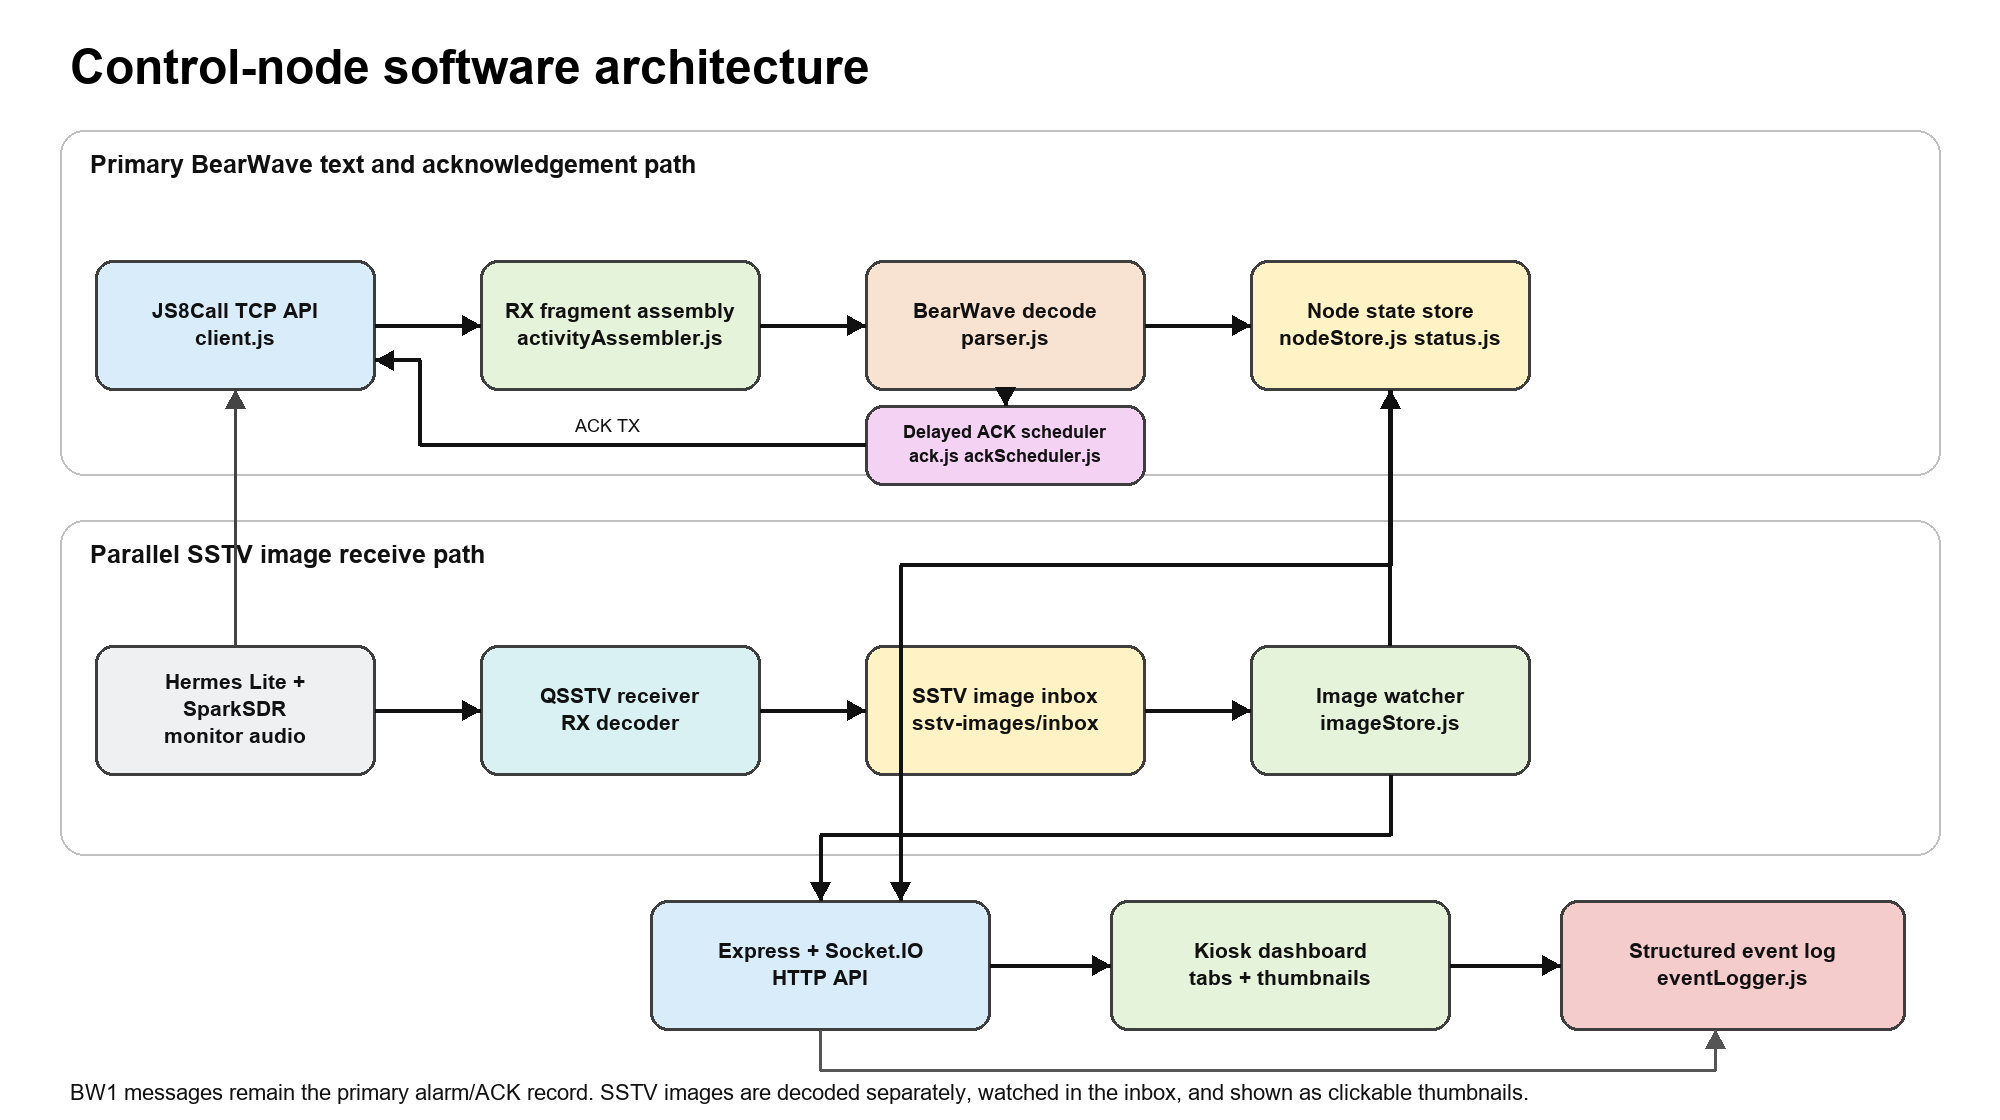
\includegraphics[width=0.95\linewidth]{images/bearwave_control_node_software_architecture.png}
    \caption{Control-node software architecture showing the receive path from JS8Call to the BearWave node-state model, the delayed acknowledgement path, the SSTV image-inbox watcher, and the browser dashboard path.}
    \Description{Block diagram with two receive paths. The primary BearWave text path runs from JS8Call TCP API input through receive fragment assembly, BearWave decoding, node-state storage, delayed acknowledgement scheduling, Express and Socket.IO delivery, dashboard display, and structured event logging. The parallel SSTV path runs from Hermes Lite and SparkSDR monitor audio through QSSTV, the SSTV image inbox, the image watcher, node-state association, the HTTP API, and the kiosk dashboard thumbnail display.}
    \label{fig:control-node-software-architecture}
\end{figure}

\begin{table}[tbp]
\caption{Principal control-node software modules.}
\label{tab:control-node-modules}
\begin{tabularx}{\linewidth}{p{0.28\linewidth}X}
\toprule
Module & Responsibility \\
\midrule
\texttt{config/default.js} & Defines web port, JS8Call host and port, heartbeat interval, grace period, alert settings, log path, acknowledgement delay, duplicate-suppression interval, and node-to-callsign mapping. \\
\texttt{src/index.js} & Orchestrates startup, receive handling, parsing, state updates, acknowledgement scheduling, HTTP service, and Socket.IO service. \\
\texttt{src/js8/client.js} & Maintains the TCP connection to JS8Call, receives newline-delimited JSON events, and sends directed messages using \texttt{TX.SEND\_MESSAGE}. \\
\texttt{activityAssembler.js} & Reconstructs complete BearWave frames from fragmented \texttt{RX.ACTIVITY} text and carries useful JS8Call context such as frequency, offset, SNR, speed, and drift. \\
\texttt{parser.js} and \texttt{types.js} & Validate the \texttt{BW1} envelope, recognise message classes, and decode compact telemetry tokens. \\
\texttt{nodeStore.js} and \texttt{status.js} & Store the latest state for each node and derive green, yellow, or red health from last-heard timing. \\
\texttt{ack.js} and \texttt{ackScheduler.js} & Build compact acknowledgements, schedule delayed directed replies, and suppress duplicate acknowledgement scheduling. \\
\texttt{src/images/imageStore.js} & Watches the SSTV image inbox, publishes image metadata, and associates newly received images with the most recent node awaiting visual evidence. \\
\texttt{httpServer.js} and \texttt{socketServer.js} & Serve the dashboard and push live updates to the browser. \\
\texttt{src/ui/public/*} & Provides the kiosk dashboard, node cards, clickable SSTV thumbnails, modal image viewer, node list, alert list, history view, and log view. \\
\texttt{scripts/start\_qsstv\_rx.sh} & Starts the QSSTV receive helper and routes the SparkSDR monitor audio to JS8Call and QSSTV with deployment-tuned levels. \\
\texttt{eventLogger.js} & Writes persistent JSON-line events for bench-test correlation and later analysis. \\
\bottomrule
\end{tabularx}
\end{table}

The receive path begins with \texttt{RX.ACTIVITY} fragments from JS8Call. Since JS8Call does not guarantee that a BearWave payload will arrive as a single complete text object, the assembler concatenates fragments until a valid \texttt{BW1} frame can be extracted. The parser then validates the message structure, confirms the message class, and converts compact telemetry tokens into structured values. The resulting message updates the node store: battery and environmental values are refreshed, alarm state is raised where applicable, and the last-heard timestamp is updated from the local receipt time.

\begin{figure}[tbp]
    \centering
    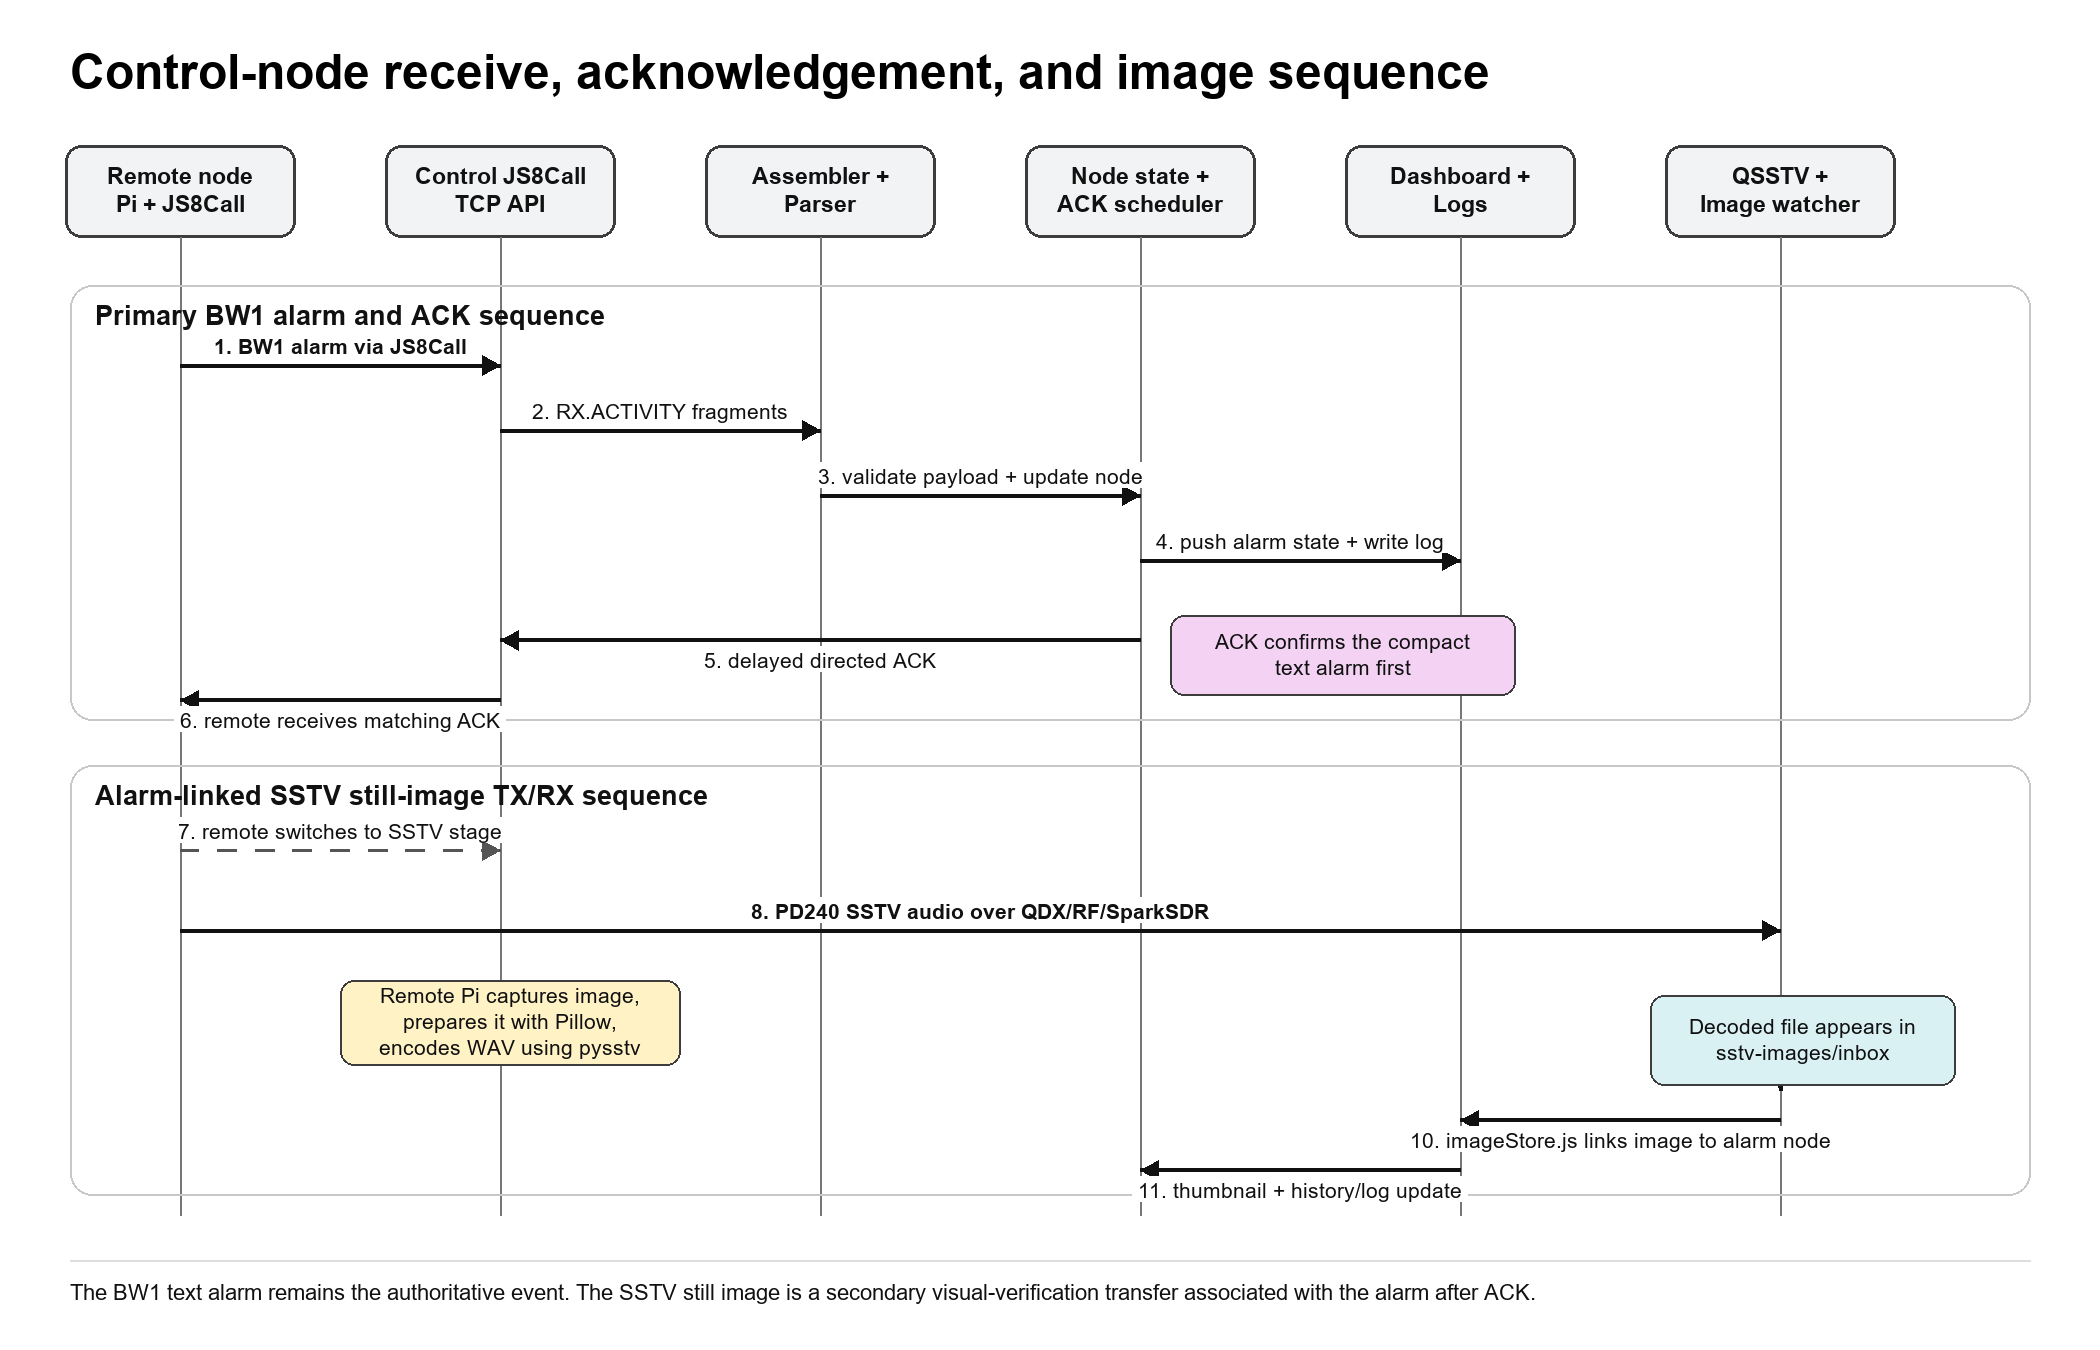
\includegraphics[width=0.95\linewidth]{images/bearwave_control_node_receive_ack_sequence.png}
    \caption{Nominal control-node receive and image sequence, from fragmented JS8Call activity to payload validation, node-state update, delayed acknowledgement scheduling, dashboard refresh, and the alarm-linked SSTV image receive path.}
    \Description{Sequence diagram with two lanes. The upper lane shows the primary BearWave alarm path: the remote node transmits a BW1 alarm through JS8Call, the control node receives fragments, assembles and validates the payload, updates node state, refreshes the dashboard and log, schedules a delayed directed acknowledgement, and the remote node receives the matching ACK. The lower lane shows the SSTV extension: after the ACK, the remote node captures and encodes a PD240 SSTV image, transmits it through the QDX and RF path, QSSTV decodes the received image, the image watcher links it to the alarm node, and the dashboard displays the clickable thumbnail.}
    \label{fig:control-node-receive-ack-sequence}
\end{figure}

The acknowledgement path is deliberately scheduled rather than immediate. Once a valid message has updated the node state, the control node constructs a compact acknowledgement of the form \texttt{A|node|message\_id}, wraps it as a directed JS8Call message using the configured node-to-callsign map, and hands it to JS8Call after a configurable delay. This delay exists because the remote node may still be completing its own transmit cycle when the control node first decodes the message. Duplicate suppression is keyed on node identifier and message identifier so that repeated decodes of the same on-air message do not schedule multiple acknowledgements.

The SSTV receive path runs alongside this message path rather than inside it. SparkSDR presents the Hermes Lite receive audio to the Linux audio system, JS8Call uses that audio for compact BearWave messages, and QSSTV uses the same received audio for image decoding. In the working configuration the receive levels were tuned down to improve reliability and reduce overdriving of the decoders. QSSTV writes decoded images into \path{sstv-images/inbox}; the control-node image watcher detects new files, emits an update over Socket.IO, exposes the image metadata through the HTTP API, and links the latest received image to the node card waiting for alarm evidence.

The operator interface is a browser-based touchscreen dashboard served by the same Node.js application and launched in kiosk mode on the control-node display. A summary bar reports the count of known nodes and their green, yellow, and red states. Each node card shows the identifier, health state, last message type, last-heard time, age since last message, decoded telemetry such as battery voltage or percentage, and the latest associated SSTV thumbnail where available. Trap and low-battery conditions are highlighted within the card and can raise a local alarm banner. The bottom navigation exposes operational views for dashboard, nodes, alerts, history, and logs, while the map view remains a placeholder for later geospatial work. The current acknowledgement and clear controls are presentation-layer actions for bench testing and usability development; they are not presented as a final field-command workflow.

\begin{figure}[tbp]
    \centering
    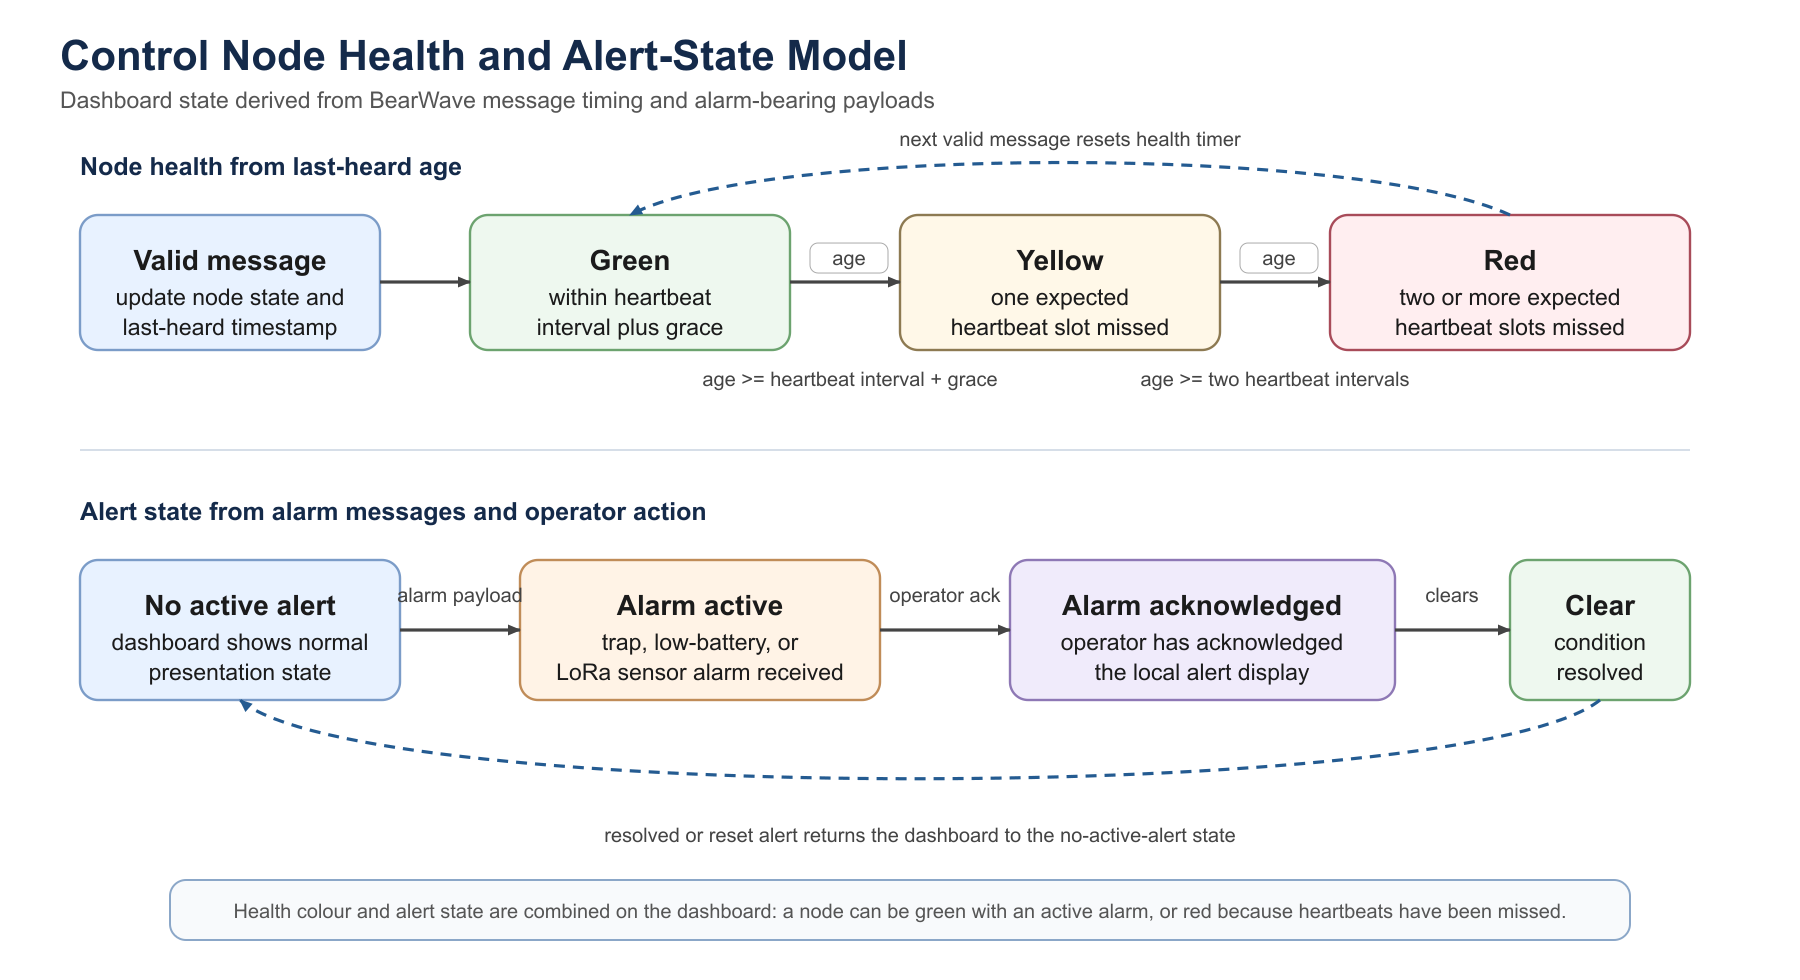
\includegraphics[width=0.95\linewidth]{images/bearwave_control_node_health_state_model.png}
    \caption{Working node-health and alert-state model used by the control node to convert receipt timing and alarm indications into operator-visible status.}
    \Description{State diagram showing green, yellow, and red node health based on last-heard age, plus active and acknowledged alarm presentation states.}
    \label{fig:control-node-health-state-model}
\end{figure}

Node health is derived from elapsed time since the last valid BearWave message. If the last-heard age is less than the configured heartbeat interval plus grace margin, the node is shown as green. If the age exceeds that threshold but remains below two complete heartbeat intervals, the node is shown as yellow. Once two heartbeat intervals have been missed, the node is shown as red. This deterministic model makes a missing heartbeat visible before the node is treated as fully offline, and it provides a simple operational rule that can be tested directly.

\begin{table}[tbp]
\caption{Control-node health and alarm-state rules.}
\label{tab:control-node-health-rules}
\begin{tabularx}{\linewidth}{p{0.24\linewidth}X}
\toprule
State & Rule and purpose \\
\midrule
Green & Last-heard age is less than heartbeat interval plus grace; the node has checked in within its expected reporting window. \\
Yellow & Last-heard age has exceeded interval plus grace but remains below two heartbeat intervals; the operator is warned that one expected heartbeat slot has been missed. \\
Red & Last-heard age is greater than or equal to two heartbeat intervals; the node is treated as having missed at least two reporting windows. \\
Alarm active & A trap alarm or alarm flag has been received and operator attention is required regardless of heartbeat colour. \\
Alarm acknowledged & The operator has locally acknowledged the alarm presentation state. \\
\bottomrule
\end{tabularx}
\end{table}

Logging is treated as part of the research design rather than as a convenience feature. The control node stores both raw JS8Call traffic and structured BearWave events, including assembled payloads, valid receive events, acknowledgement scheduling, acknowledgement handoff, acknowledgement success or failure, and duplicate-suppression events. These logs provide UTC-labelled points that can be aligned with remote-node logs during bench testing. Importantly, this diagnostic detail remains local to the control node rather than being added to the RF payload.

\subsection{Control Node Validation}
Control-node validation demonstrates that each software boundary works before the system is treated as field ready. The most important tests are receive-fragment assembly, message validation, node-state update, delayed acknowledgement timing, duplicate suppression, dashboard update, and persistent logging. These tests can initially be performed using simulated JS8Call JSON events and known BearWave payloads before being repeated over the full radio path.

\begin{table}[tbp]
\caption{Validation checks for the control-node prototype.}
\label{tab:control-node-validation}
\begin{tabularx}{\linewidth}{p{0.25\linewidth}XX}
\toprule
Check & Method & Evidence \\
\midrule
JS8Call API connectivity & Start JS8Call and verify that the Node.js client receives newline-delimited JSON events from the TCP API. & Raw JS8Call event log and service status output. \\
Fragment assembly & Feed known fragmented \texttt{RX.ACTIVITY} text into the assembler. & One reconstructed \texttt{BW1} payload with preserved JS8 context. \\
Protocol validation & Submit valid and malformed BearWave frames. & Valid frames update node state; malformed frames are rejected and logged. \\
Delayed ACK scheduling & Decode a known message and measure the interval before \texttt{TX.SEND\_MESSAGE}. & Structured \texttt{BW\_ACK\_SCHEDULED} and handoff log entries. \\
Duplicate suppression & Replay the same node/message pair within the suppression window. & One acknowledgement is scheduled and duplicates are logged as suppressed. \\
Dashboard update & Validate a heartbeat, low-battery event, and trap alarm. & Node card, summary counts, and alarm banner update without browser reload. \\
SSTV image receive & Place or decode a known image into the configured image inbox after an alarm event. & Image metadata appears through the HTTP API and the node card displays a clickable thumbnail. \\
Kiosk startup & Reboot the control node with autostart enabled. & SparkSDR, JS8Call, QSSTV/audio routing, control service, and Chromium kiosk dashboard start automatically. \\
Restart recovery & Restart the service and repeat known-message tests. & Service reconnects to JS8Call and resumes logging and dashboard delivery. \\
\bottomrule
\end{tabularx}
\end{table}

The paper treats the current limitations of the control-node prototype explicitly. The node-state store is in memory, image-to-node association currently depends on the temporal relationship between an alarm and the following SSTV file, and the acknowledgement delay is manually tuned during bench testing. These are acceptable for a research prototype because they keep the system transparent and easy to inspect, but they also define clear future work: persistent multi-node state, explicit image acknowledgements, authenticated remote command workflows, formal configuration tooling, and wider validation across different JS8Call and SSTV timing conditions.

\section{Remote Node Hardware Design}

\subsection{Remote Node Overview}
The BearWave remote node PCB is designed as an integrated control, sensing, timing, communications, image-capture, and power-management board for a field-deployed monitoring system. The design combines a Heltec WiFi LoRa 32 V3 module, a Raspberry Pi Zero 2 W, camera module, GPS, real-time clock backup, trap switch inputs, battery monitoring, switched 5 V and 12 V power rails, and an external low-power HF radio chain based on a QRP Labs QDX, modified ATU100 tuner, and inverted-V dipole. The PCB is a four-layer board and is currently on revision 2.

\begin{figure}[tbp]
    \centering
    \makebox[\linewidth][c]{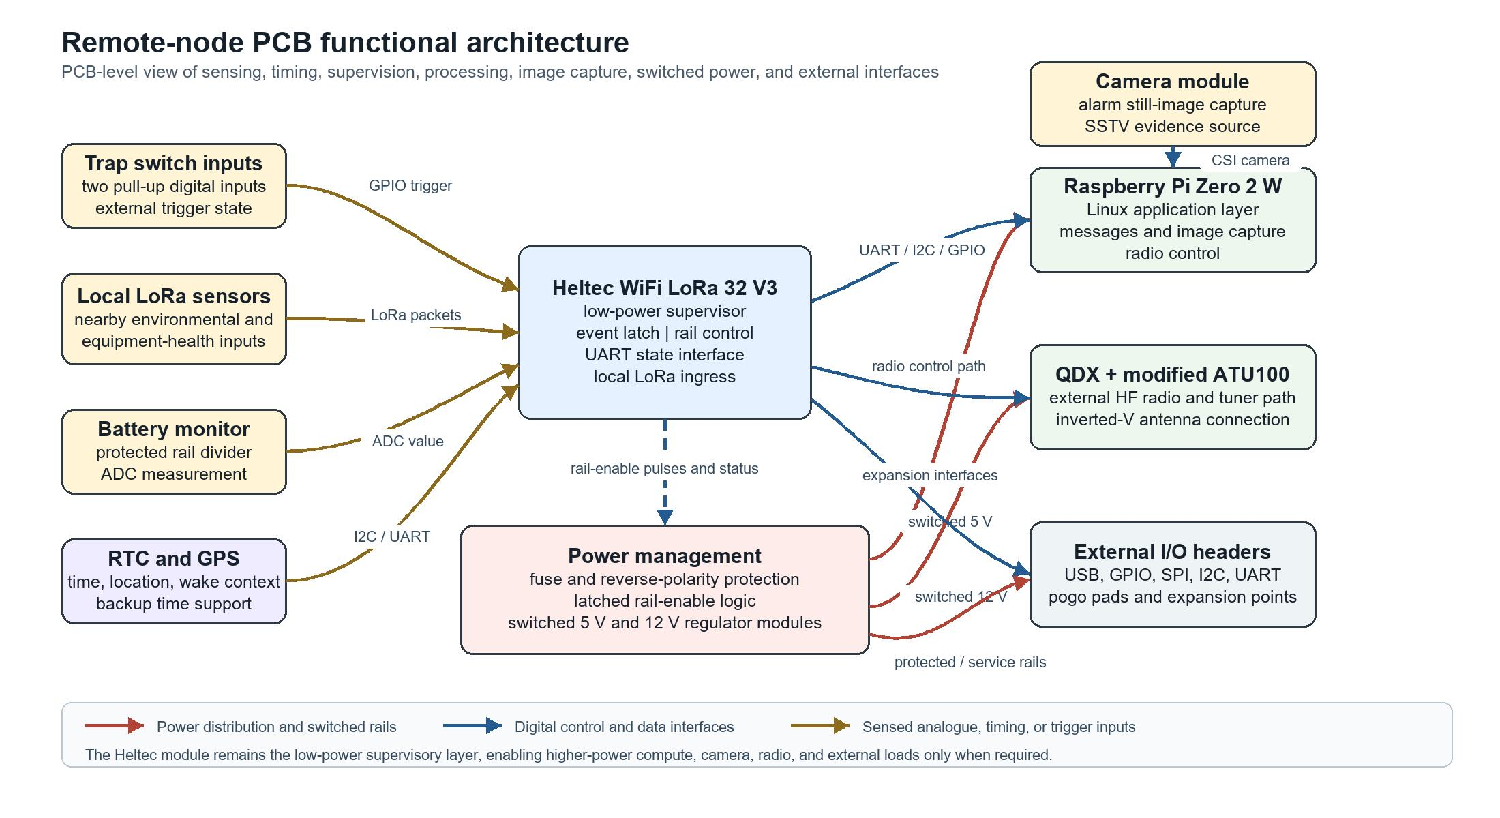
\includegraphics[width=1.15\linewidth]{images/bearwave_pcb_functional_architecture.pdf}}
    \caption{PCB-level functional architecture of the BearWave remote node, showing how sensing, timing, supervision, camera image capture, higher-level processing, switched power distribution, and external interfaces are organised on and around the board.}
    \Description{Functional block diagram of the BearWave remote-node PCB. Trap switches, LoRa sensors, battery monitoring, RTC, and GPS feed the Heltec supervisor. The supervisor controls the power-management block and exchanges control data with the Raspberry Pi, radio path, and external input-output headers. A camera module is shown as a separate alarm-image source connected to the Raspberry Pi Zero 2 W through the CSI camera interface for SSTV evidence capture.}
    \label{fig:pcb-functional-architecture}
\end{figure}

\begin{figure}[tbp]
    \centering
    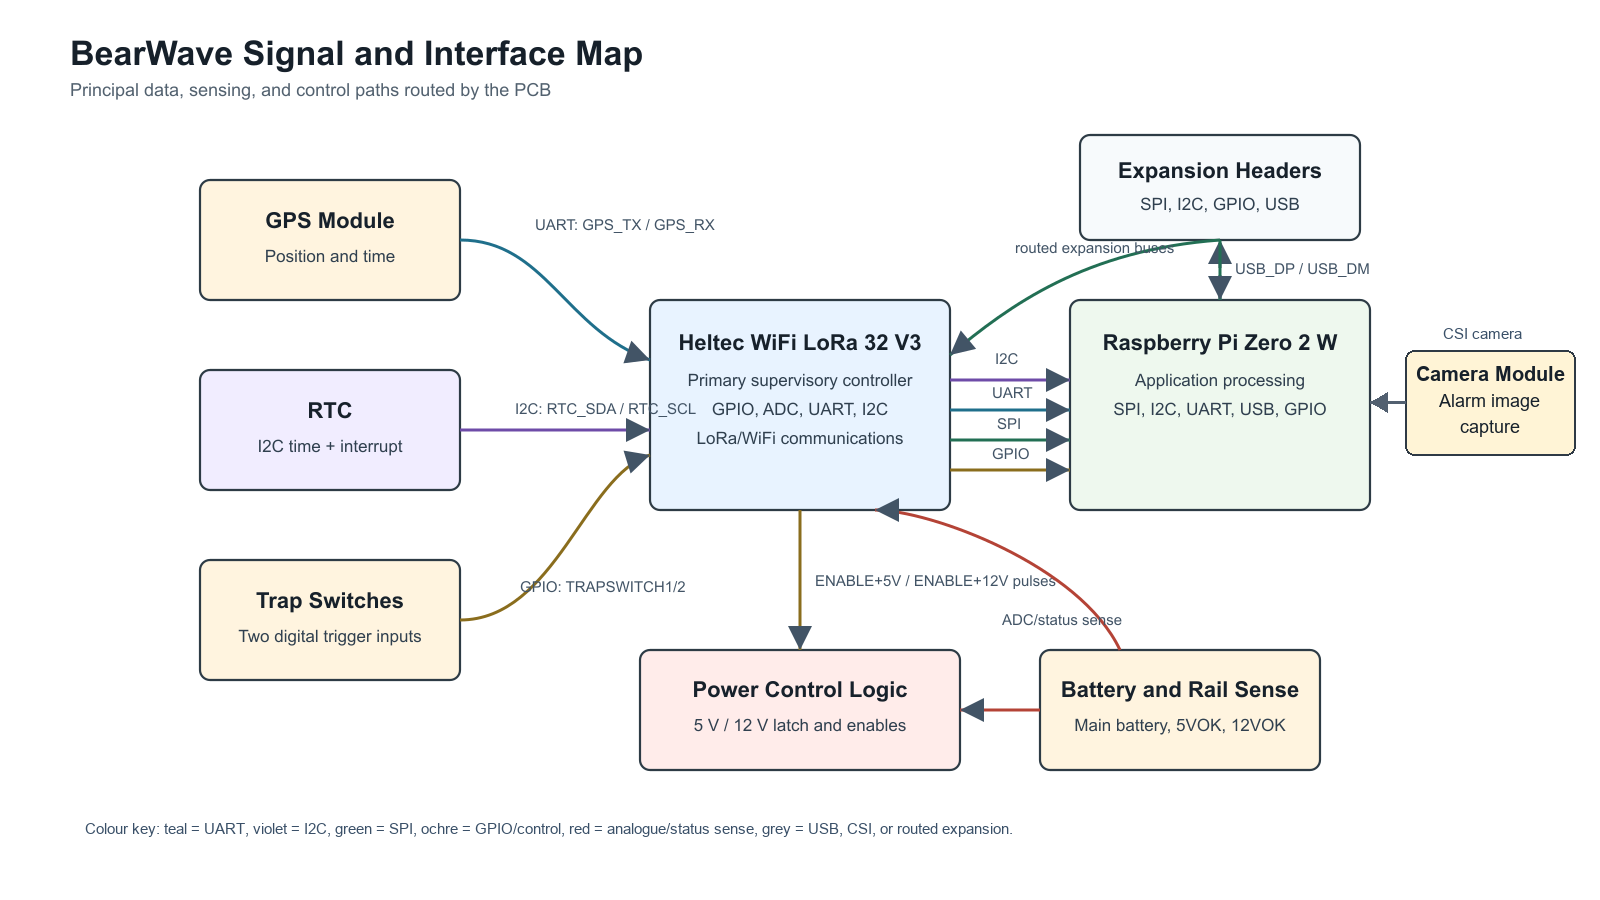
\includegraphics[width=0.95\linewidth]{images/bearwave_signal_interfaces_diagram.png}
    \caption{Remote node signal interfaces, including local sensing, timing, controller, Raspberry Pi, camera, and external communication pathways.}
    \Description{Signal interface diagram for the BearWave remote node, showing connections between controller, timing, sensing, camera, and communication subsystems. The camera module is connected to the Raspberry Pi Zero 2 W through a CSI camera interface and provides the alarm-image input used by the SSTV extension.}
    \label{fig:signal-interfaces}
\end{figure}

\subsection{Supervisory Controller and Compute Module}
The main system controller is the Heltec WiFi LoRa 32 V3, which provides low-power microcontroller control, LoRa radio communication, Wi-Fi capability, GPIO monitoring, and power-rail supervision. It receives inputs from trap switches, the GPS module, the RTC interrupt line, the main battery-voltage divider, and the 5 V/12 V rail status outputs. It also provides the schematic-defined \texttt{ENABLE5VPULSE} and \texttt{ENABLE12VPULSE} firmware-control signals for the 5 V and 12 V rail latch circuitry. The Heltec LoRa radio supports local sensor expansion: nearby low-power sensor devices can report measurements to the remote node over LoRa, after which the BearWave node can package the relevant values into its HF message without requiring changes to the main remote-node hardware.

A Raspberry Pi Zero 2 W is included as a higher-level processing module. The PCB routes its UART, I2C, SPI, USB, power, and GPIO connections to headers, allowing it to interface with external peripherals and the Heltec controller. The Pi is powered from the regulated 5 V rail and is used when more computational capability is required than the Heltec can provide alone.

The Pi remains necessary because the current BearWave radio path depends on mature Linux-hosted software for JS8Call operation, message orchestration, logging, acknowledgement matching, and interaction with the QDX radio interface. The ESP32 is not intended to run the FT8-derived JS8Call signal-processing and radio-control stack: it lacks the computing resources, operating-system support, and software ecosystem required for that role. The design therefore accepts the Pi's boot time and energy cost, while using the ESP32 to limit that cost to short communication windows.

\subsection{Power Protection and Switched Rails}
Power enters the board through the main battery connection and passes through fuse protection and an LTC4358-based reverse-polarity/ideal-diode protection stage. This produces a protected \texttt{M\_BAT\_OUT} rail. The protected battery rail feeds two XL6019 buck-boost regulator modules that generate regulated 5 V and 12 V supplies. The 5 V rail powers the Raspberry Pi and other 5 V circuitry, while the 12 V rail is routed through an output fuse for external 12 V loads. Voltage dividers provide electrical confirmation that the 5 V and 12 V rails are present. Indicator LEDs are also provided for bench testing and faultfinding, but they are connected through removable links so they can be disconnected before deployment and do not consume power in the field.

The 5 V and 12 V supplies are switchable under both manual and firmware control. Manual pushbuttons and separate Heltec-generated enable signals are combined through logic gates and fed into a dual D-type flip-flop latch. This allows each rail to be controlled independently while retaining a latched on/off state. A reset supervisor defines the startup state of the latch circuitry so that the power system begins in a known condition, and BSS138 MOSFETs interface the latch outputs to the enable pins of the buck-boost modules. This arrangement lets the system conserve battery power by energising higher-power subsystems only when required.

\begin{figure}[tbp]
    \centering
    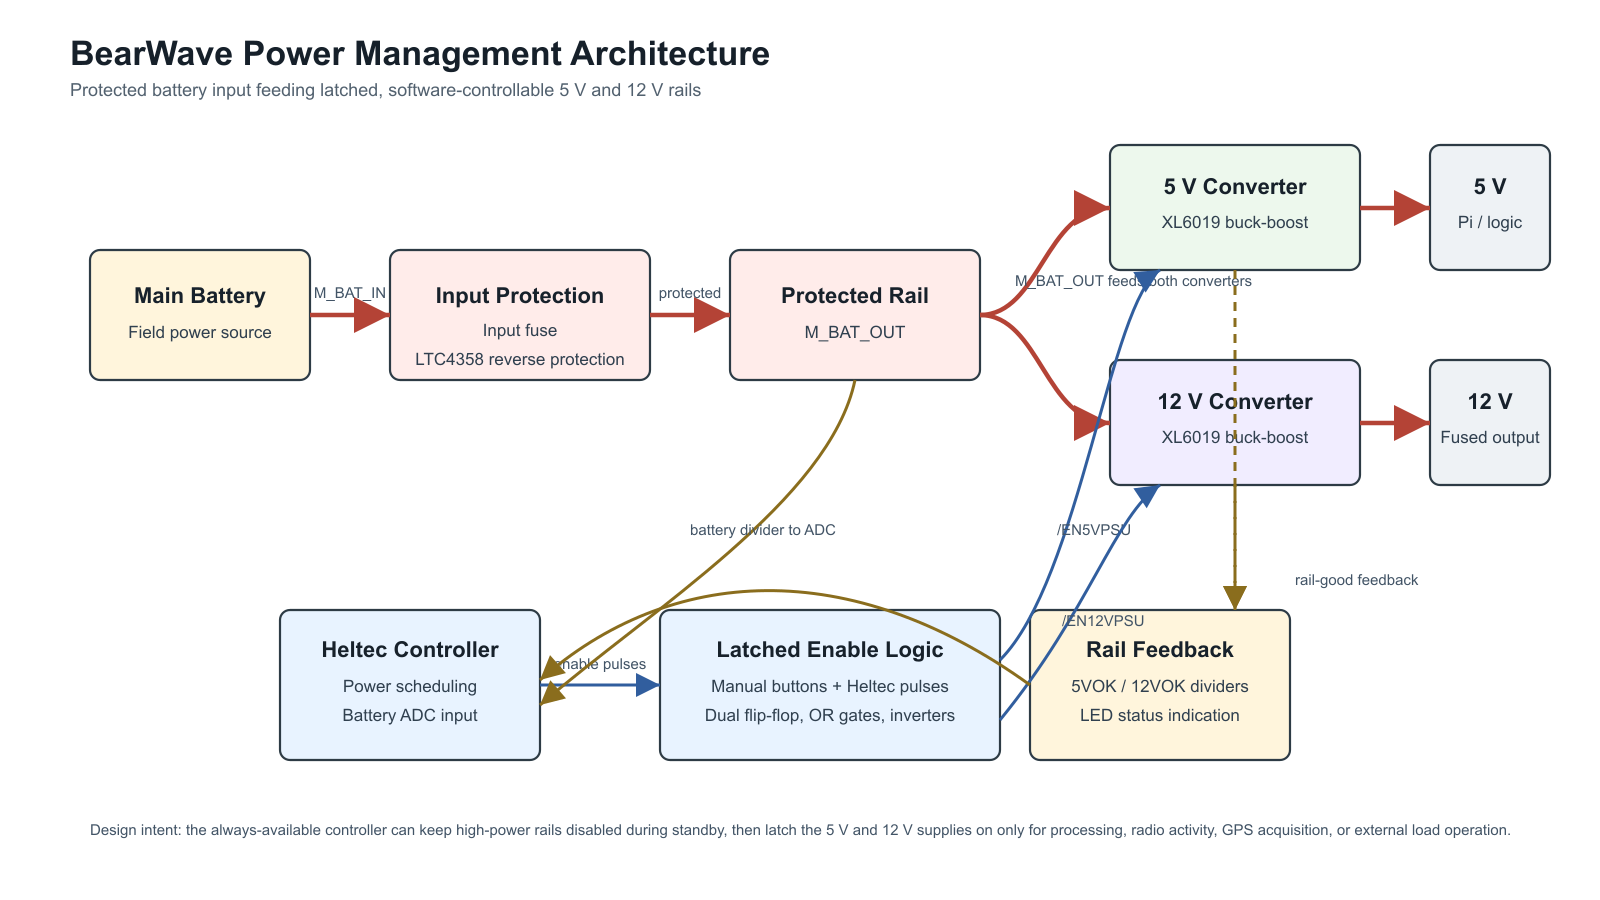
\includegraphics[width=0.95\linewidth]{images/bearwave_power_management_diagram.png}
    \caption{Remote node power-management architecture showing protected battery input, switched regulated rails, manual controls, and firmware-controlled rail enable paths.}
    \Description{Power-management diagram showing battery protection, regulated rails, manual controls, and firmware-controlled switching.}
    \label{fig:power-management}
\end{figure}

\subsection{HF Radio and Antenna Subsystem}
The remote-node radio subsystem is the hardware bridge between the Raspberry Pi software stack and the long-haul HF/NVIS link. In the current design this subsystem consists of three main elements: a QRP Labs QDX digital transceiver, a modified ATU100 automatic antenna tuner, and an inverted-V dipole antenna. The QDX provides the low-power digital-mode transceiver used by the Pi and JS8Call stack, while the ATU100 provides antenna matching between the transceiver and the field antenna. The inverted-V dipole is the deployed antenna geometry selected for NVIS-style propagation and practical installation in field conditions where vertical supports may be improvised from trees, poles, or existing site structures.

The radio chain is deliberately separated from the low-power ESP32 supervisory layer. The ESP32 does not generate or decode the HF signal; its role is to decide when the radio path is powered, to provide event state to the Pi, and to shut the high-load hardware down at the end of the communication cycle. The Raspberry Pi then controls the communication session through JS8Call and the QDX. This separation preserves the low-power duty cycle: the radio hardware is treated as an intermittent high-energy subsystem rather than as an always-on receiver.

The modified ATU100 is important because the remote node is intended to operate in a QRP power envelope below 10 W. Standard automatic tuner behaviour may assume a higher RF drive level for reliable detection and tuning, which is not well matched to a battery-powered conservation node. The BearWave version therefore uses a modified ATU100 arrangement so that antenna matching can be performed at the lower power levels available from the QDX-based system. The modification is part of the reproducible hardware design rather than an incidental bench change, because tuning reliability directly affects message success, energy use, and field serviceability.

\begin{table}[tbp]
\caption{Remote-node HF radio and antenna subsystem.}
\label{tab:remote-rf-subsystem}
\begin{tabularx}{\linewidth}{p{0.24\linewidth}X}
\toprule
Element & Role and design implication \\
\midrule
QRP Labs QDX & Low-power digital transceiver used by the Raspberry Pi and JS8Call stack to transmit BearWave messages over HF, and by the optional SSTV stage to transmit the generated image waveform. It forms the main radio interface for the remote node. \\
Modified ATU100 & Provides antenna matching between the QDX and the field antenna at sub-10 W operating levels. The low-power modification and tuning workflow are part of the reproducible hardware record. \\
Inverted-V dipole & Provides the remote-node HF/NVIS antenna arrangement. Its deployment geometry is recorded because feed-point height, end height, ground proximity, and surrounding vegetation affect performance. \\
Switched power rail & Powers the radio/tuner subsystem only during communication windows, reducing standby consumption. The build record identifies whether the QDX and ATU100 share the switched 12 V rail or use a separate regulated radio rail. \\
Pi-to-radio interface & Allows JS8Call on the Raspberry Pi to hand the compact BearWave payload to the QDX for transmission and allows the SSTV transmit script to play the generated audio waveform through the same configured audio path. The build record includes USB/audio/CAT interface details, device naming, permissions, audio-level settings, and startup order. \\
Antenna feed and matching path & Connects QDX output to the ATU100 and then to the inverted-V dipole. This path is validated for SWR, tuner success rate, insertion loss, connector robustness, and weatherproofing. \\
\bottomrule
\end{tabularx}
\end{table}

From a system perspective, the RF subsystem introduces three additional evaluation constraints. First, the tuner must be able to find and retain a usable match at the actual operating power. A failed or slow tune would increase active time and may prevent successful message delivery. Second, the antenna installation is part of the communication system, not a background detail. An inverted-V dipole deployed at a different height or with different end geometry may change NVIS performance, impedance, losses, and repeatability. Third, the QDX, ATU100, Raspberry Pi, and any supporting interface hardware are included in the remote-node power budget, both during transmit and during any receive/acknowledgement window.

The RF validation record includes QDX transmit power, QDX receive current, ATU100 tuning current, ATU100 standby current, tuning time, SWR before and after tuning, band or frequency, dipole dimensions, feedline type, choke or balun arrangement, feed-point height, end height, and field mounting method.

\subsection{Timing, Location, and Sensor Interfaces}
The design includes a DS3231M+ real-time clock with a CR1225 backup cell. This provides accurate timekeeping even when the main system power is removed. The RTC communicates over I2C and provides an interrupt or square-wave output to the controller, allowing scheduled wake-up or time-based events.

A GPS module is connected via UART and includes its own rechargeable backup battery connection. This allows the system to obtain position and time information while retaining GPS backup state between power cycles. The GPS is powered from the switched 3.3 V supply, enabling the controller to disable it when not needed.

GPS reception cannot be assumed in all conservation deployments because canopy cover, terrain, enclosure placement, or temporary sky-view obstruction may prevent a valid satellite lock. The ESP32 therefore treats the RTC as the continuing local time source when GPS time is unavailable. When the GPS has a valid lock, the ESP32 compares GPS-derived UTC with the DS3231M+ RTC value and resynchronises the RTC if a time offset is detected. This allows the Raspberry Pi \texttt{TIME?} request to receive a usable UTC time from the RTC during periods without GPS coverage, while opportunistically correcting RTC drift whenever GPS time becomes available again.

Two trap switch inputs are provided using pull-up resistors to 3.3 V, with the external switches pulling the input lines to ground when activated. These inputs are routed to Heltec GPIO pins and can be used to detect trap state changes or external trigger events. Battery monitoring is implemented using a high-value resistor divider and filter capacitor connected to the protected main battery output. This scales the battery voltage to a safe ADC range for the Heltec, allowing firmware to estimate battery state and make power-management decisions.

The alarm-image extension adds a Raspberry Pi camera module as a Pi-side sensor interface rather than as part of the ESP32 supervisory layer. The camera connects to the Raspberry Pi Zero 2 W through the CSI camera interface and is powered only while the Pi is awake. It is used after an acknowledged alarm to capture a still image for the optional SSTV evidence path; routine alarm validity still comes from the compact BearWave message and acknowledgement rather than from successful image reception.

The same node design also supports wireless local sensing through the Heltec LoRa interface. This is distinct from the long-haul HF/NVIS path: LoRa is used locally around a remote node, while HF is used to carry selected alarms and telemetry back to the control node. LoRa-connected sensors such as temperature, humidity, contact, or equipment-health modules are normalised by the ESP32 firmware and exposed to the Raspberry Pi using the same compact state-query pattern as wired events. This keeps sensor expansion primarily in firmware and configuration, avoiding hardware changes to the BearWave PCB for each new sensor type.

\subsection{Schematic and Design Files}
Figure~\ref{fig:pcb-assembled-photos} shows the assembled revision 2 remote-node PCB used for validation, including both the component side and reverse side of the board. These photographs document the physical relationship between the Heltec module, Raspberry Pi Zero 2 W, power regulation modules, headers, battery/RTC area, service points, and labelled field connectors on the built hardware.

\begin{figure}[tbp]
    \centering
    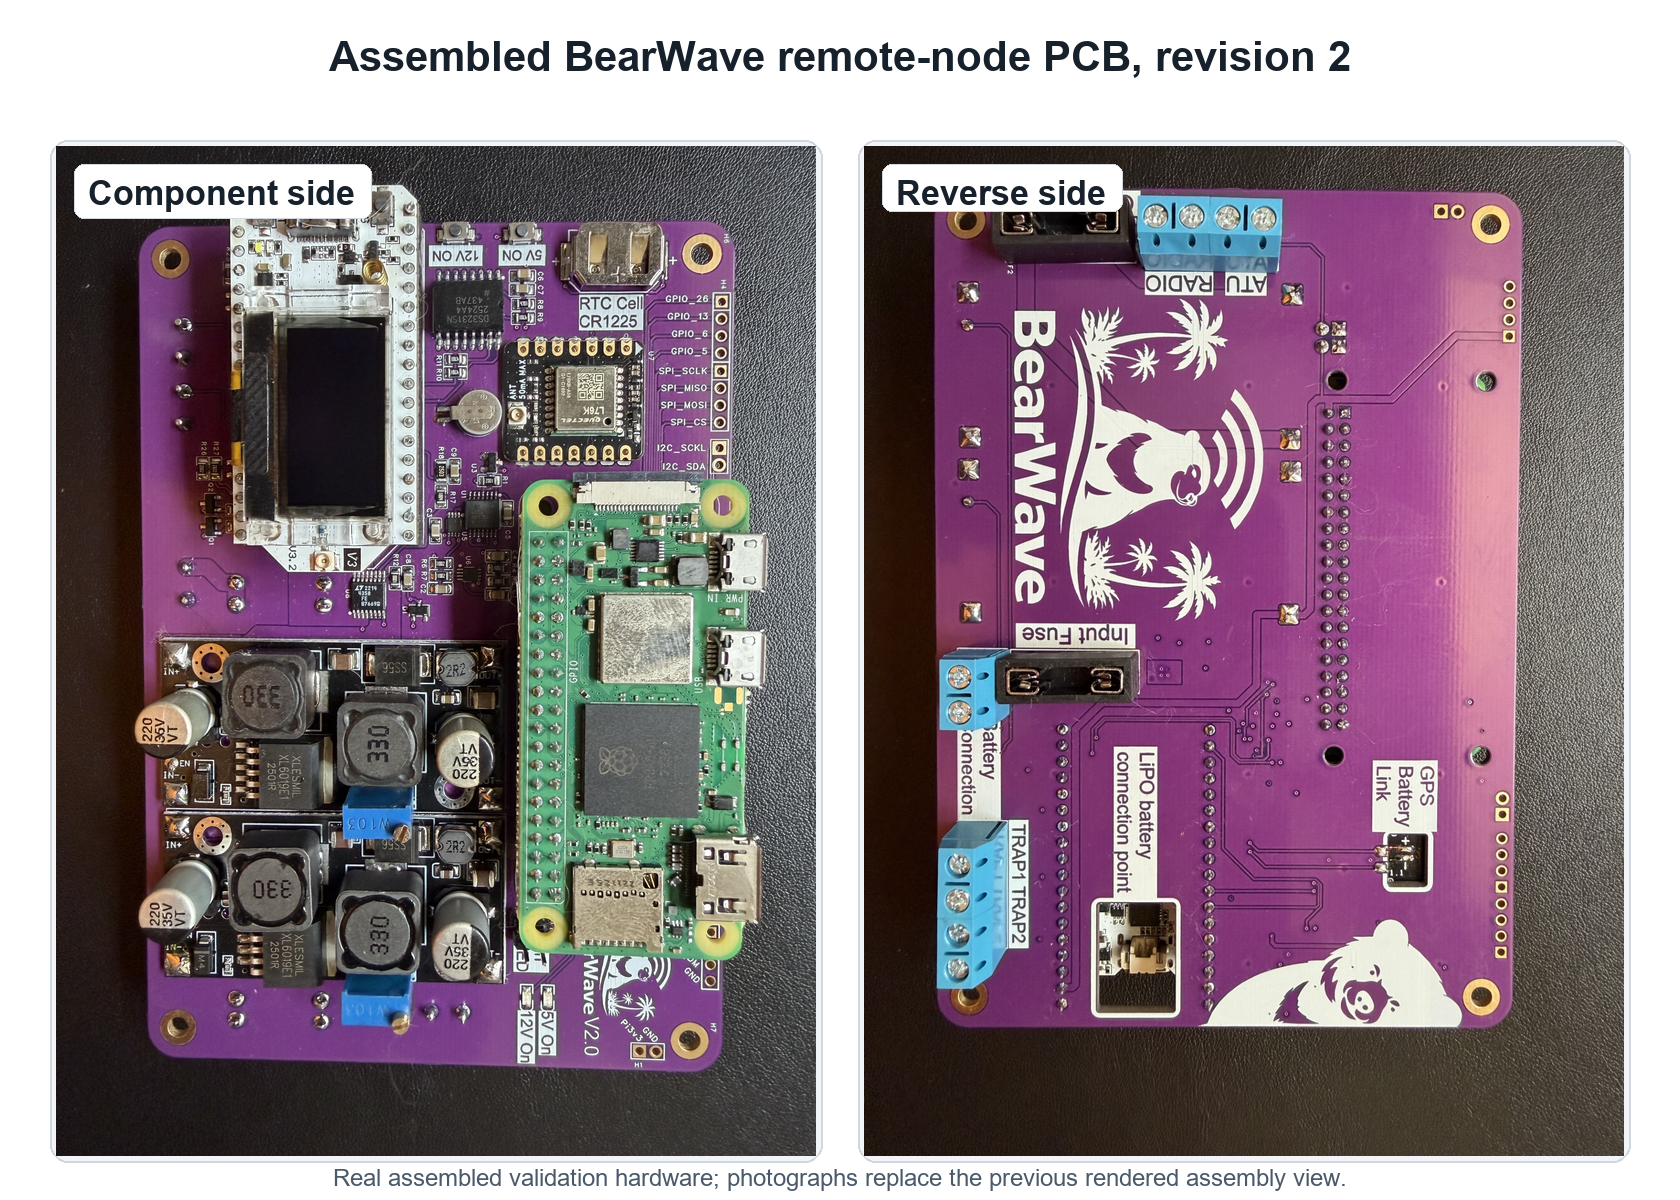
\includegraphics[width=0.98\linewidth]{images/bearwave_remote_node_real_pcb_both_sides.png}
    \caption{Photographs of the assembled revision 2 BearWave remote-node PCB, showing the component side and reverse side of the validation hardware.}
    \Description{Two-panel photograph of the assembled BearWave revision 2 remote-node printed circuit board. The component side shows the Heltec ESP32 module, Raspberry Pi Zero 2 W, power regulation modules, RTC battery area, headers, buttons, and labelled 5 V and 12 V controls. The reverse side shows the BearWave board artwork, field connectors, trap inputs, battery connection, GPS battery link, LiPo battery connection point, header soldering, and board routing.}
    \label{fig:pcb-assembled-photos}
\end{figure}

\begin{figure}[tbp]
    \centering
    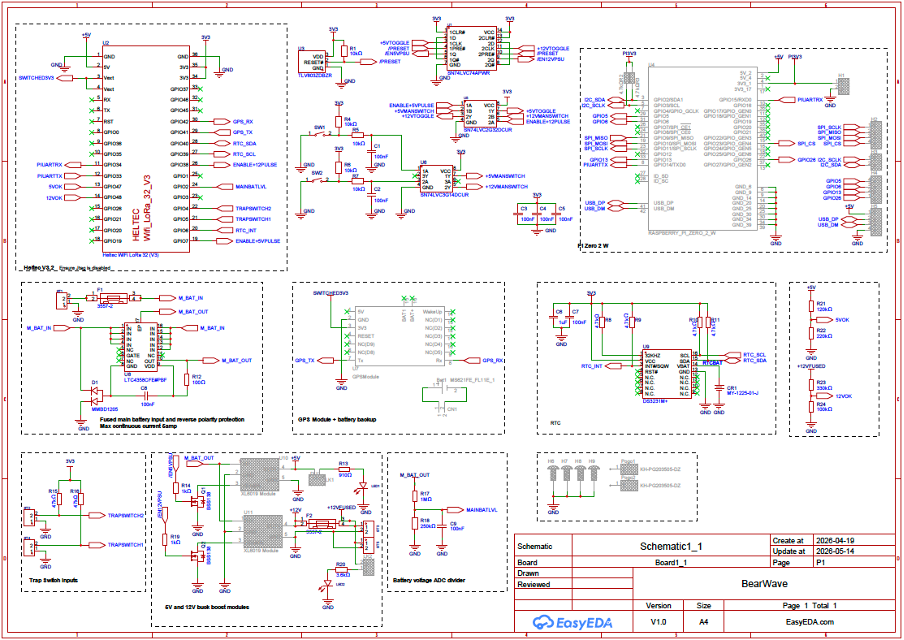
\includegraphics[width=0.95\linewidth]{images/Schematic.png}
    \caption{Current remote-node schematic overview included in the released design files.}
    \Description{Overview schematic of the current BearWave remote-node circuit.}
    \label{fig:schematic}
\end{figure}

The BearWave Paper 3 repository provides the open-hardware and software artefacts needed to audit and reproduce the build, including PCB source files, schematic, Gerbers, bill-of-materials information, firmware, Raspberry Pi software, control-node software, and example configuration files \cite{BearWaveRepository}.

\subsection{Enclosure and Ruggedisation Status}
The physical enclosure remains the least mature part of the final remote-node design. This does not prevent the electronic and software architecture from being documented, but the paper treats enclosure design candidly as remaining ruggedisation work. The final enclosure must protect the PCB, battery wiring, future sensor cable exits or field connectors, QDX/ATU100 interface, antenna exit, and service access points from rain, condensation, insects, handling damage, and wildlife interference. It must also allow repeatable antenna and cable routing, because RF performance and waterproofing are both affected by the physical exit points from the housing.

\section{Remote Node Firmware and Software}

\subsection{ESP32/Heltec Supervisory Firmware}
The ESP32/Heltec firmware description reflects the current supervisor firmware and accompanying documentation, with earlier design notes used only to recover rationale and diagrams. Pin assignments, battery thresholds, UART settings, event commands, shutdown timing, and wake-interval behaviour are therefore described as implemented in the current code base.

The ESP32 firmware acts as the hardware authority within the BearWave remote node. It is deliberately separated from the Raspberry Pi application layer: the ESP32 manages hardware state, local time, event inputs, battery context, and power sequencing, while the Raspberry Pi manages JS8Call, BearWave message construction, acknowledgement handling, retry behaviour, and application-level decision making. This division is central to the low-duty-cycle design. The Pi and radio are comparatively high-load subsystems, so they are powered only during a message cycle; the ESP32 remains available as the low-power supervisory controller that wakes the node, exposes local state to the Pi, and returns the hardware to a low-power state after communication has completed.

\begin{figure}[tbp]
    \centering
    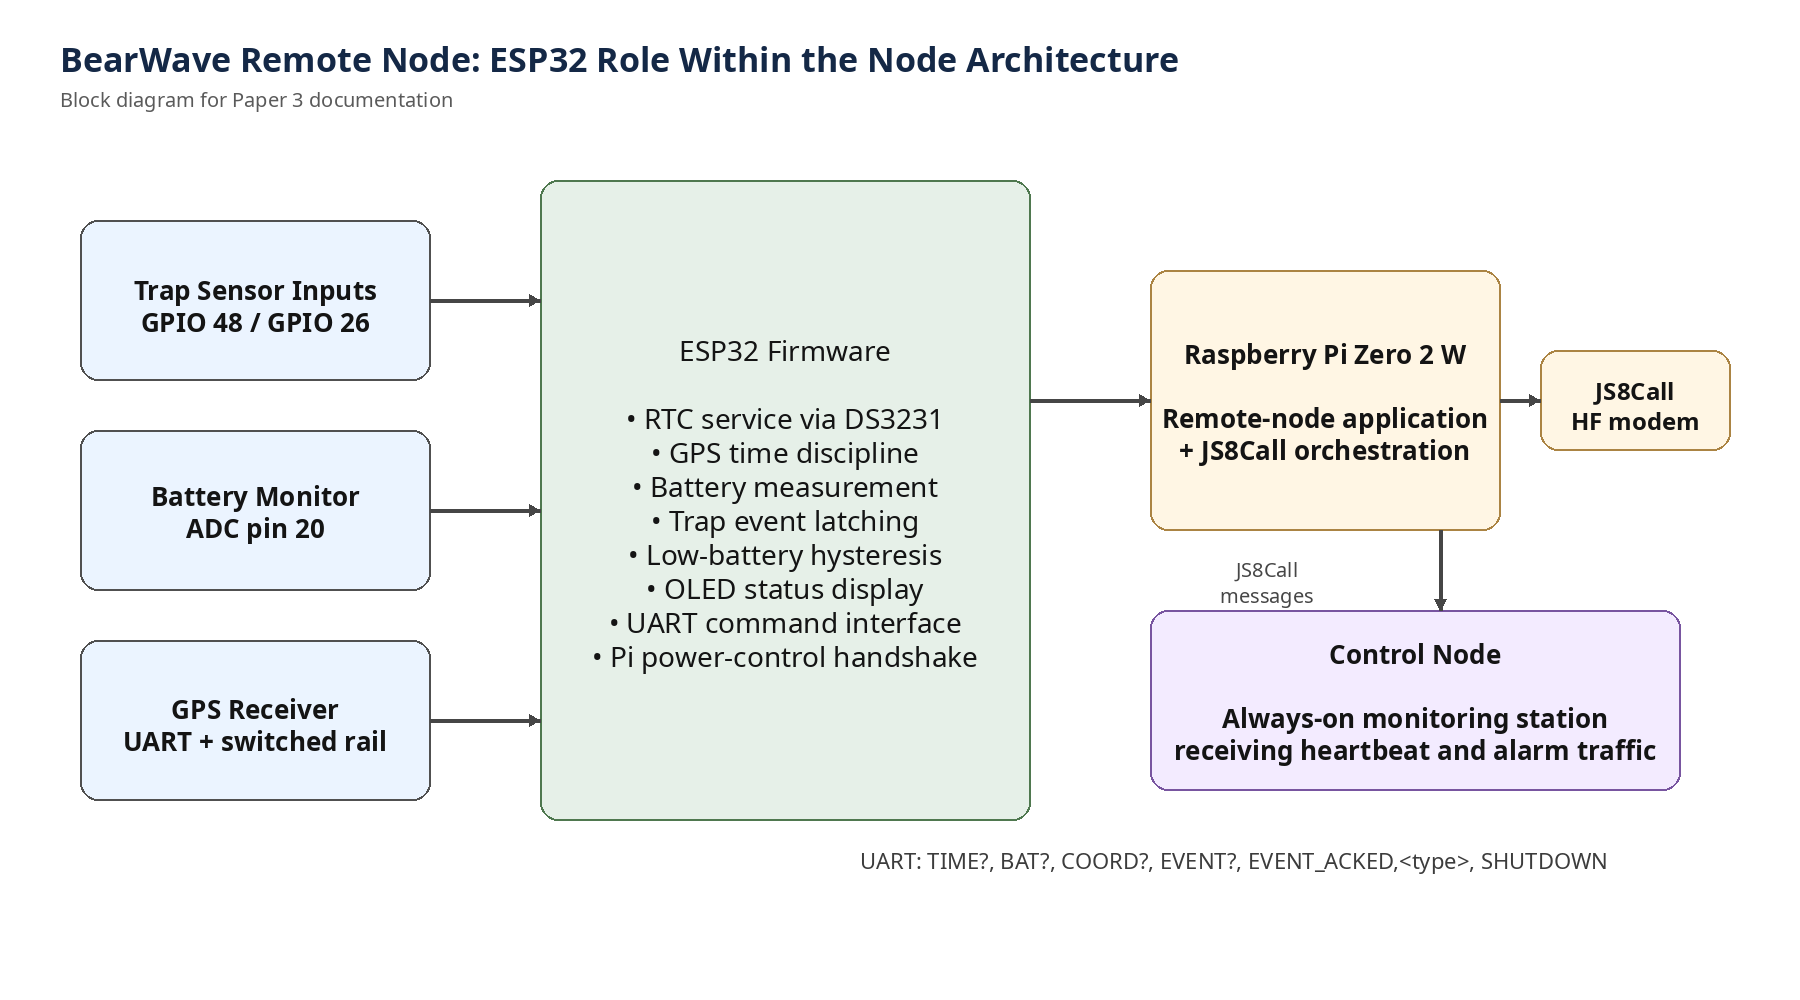
\includegraphics[width=0.95\linewidth]{images/bearwave_esp32_supervisor_architecture.png}
    \caption{ESP32 role within the BearWave remote-node architecture. The ESP32 supervises local hardware state and exposes a compact UART interface to the Raspberry Pi radio/application layer.}
    \Description{Block diagram showing trap sensor inputs, battery monitor, and GPS receiver feeding the ESP32 firmware, which communicates with a Raspberry Pi Zero 2 W, JS8Call modem, and control node.}
    \label{fig:esp32-supervisor-architecture}
\end{figure}

\begin{table}[tbp]
\centering
\caption{ESP32 supervisory firmware context.}
\label{tab:esp32-supervisor-context}
\begin{tabularx}{\textwidth}{p{0.24\textwidth}X}
\toprule
Field & Description \\
\midrule
Platform & Heltec ESP32 with OLED, DS3231 RTC, GPS receiver, battery measurement, Raspberry Pi UART, trap inputs, and independently switched 5 V and 12 V rails. \\
Primary role & Low-power hardware supervisor for the BearWave remote node. \\
Power control & The schematic-defined \texttt{ENABLE5VPULSE} and \texttt{ENABLE12VPULSE} GPIO lines provide firmware-controlled inputs to the 5 V and 12 V rail latch circuitry. \\
Latch model & The rail-control signals feed D-type flip-flop latch circuitry, allowing rail state to be held and reset to a known startup condition. \\
Sleep model & After Pi shutdown, the ESP32 commands the required rails off through the latch logic and wakes on the configured timer. \\
Companion software & Raspberry Pi remote-node Python application, JS8Call, and the BearWave control node. \\
\bottomrule
\end{tabularx}
\end{table}

\subsubsection{Power Control and Deep Sleep}
The revised power-control logic separates the 5 V and 12 V enable paths rather than treating the Raspberry Pi and radio supply as a single shared rail. The ESP32 provides independent firmware-controlled \texttt{ENABLE5VPULSE} and \texttt{ENABLE12VPULSE} signals for the two rail-control paths, while manual controls remain available for bench and service use. These signals feed the D-type flip-flop latch circuitry shown in the schematic, allowing the selected rail state to be held without relying only on the instantaneous ESP32 GPIO state.

This latch-based arrangement is important for low-power operation because the circuit can start from a known state and preserve the intended rail state across sleep and reset boundaries. During a normal wake cycle, the firmware enables the 5 V rail for the Raspberry Pi and, where required, the 12 V rail for external radio or auxiliary loads. After receiving \texttt{SHUTDOWN} from the Pi, the ESP32 waits for the configured Linux shutdown interval, commands the relevant rails off through the latch logic, isolates the Pi UART pins, and enters deep sleep.

\begin{table}[tbp]
\centering
\caption{ESP32-managed rail power cycle.}
\label{tab:esp32-power-cycle}
\begin{tabularx}{\textwidth}{p{0.08\textwidth}p{0.28\textwidth}X}
\toprule
Step & ESP32 action & Purpose \\
\midrule
1 & Wake from power-on or timer & Start a new remote-node cycle. \\
2 & Check latched rail state & Confirm that the power-control circuit is in the expected state. \\
3 & Assert \texttt{ENABLE5VPULSE}, and \texttt{ENABLE12VPULSE} when required & Power the Raspberry Pi and any required external load. \\
4 & Serve UART commands & Provide time, battery, coordinates, event state, and shutdown handling. \\
5 & Receive \texttt{SHUTDOWN} & Begin managed power-down after Pi completion. \\
6 & Wait 50 seconds & Allow the Raspberry Pi to halt cleanly. \\
7 & Command rail latch outputs off & Remove power from the Pi and any enabled external load. \\
8 & Isolate Pi UART pins & Reduce risk of back-powering the Pi through UART lines. \\
9 & Enter deep sleep & Keep low-power supervision active until the next wake condition. \\
\bottomrule
\end{tabularx}
\end{table}

\subsubsection{Hardware State Exposed to the Raspberry Pi}
The ESP32 exposes a line-based UART command set to the Raspberry Pi. This allows the Pi to treat the ESP32 as the authoritative local source for time, battery state, event state, coordinates, and shutdown control. The interface is deliberately simple, textual, and deterministic so that it remains easy to test from Python and diagnose during bench integration.

\begin{table}[tbp]
\centering
\caption{UART command interface exposed by the ESP32 supervisor.}
\label{tab:esp32-uart-commands}
\footnotesize
\begin{tabularx}{\textwidth}{p{0.21\textwidth}p{0.30\textwidth}X}
\toprule
Command & Response & Purpose \\
\midrule
\texttt{PING} & \texttt{PONG} & Basic liveness check. \\
\texttt{STATUS?} & \texttt{OK,BEARWAVE\_RTC\_GPS\_EVENTS} & Confirms expected firmware capability. \\
\texttt{TIME?} & \texttt{TIME,YYYY-MM-DDTHH:MM:SSZ} & Provides UTC time from RTC/GPS. \\
\texttt{BAT?} & \texttt{BAT,VOLTAGE,PERCENT} & Provides battery telemetry. \\
\texttt{COORD?} & \texttt{COORD,LAT,LON} or \texttt{COORD,INVALID} & Provides GPS coordinates when valid. \\
\texttt{EVENT?} & \begin{tabular}[t]{@{}l@{}}\texttt{EVENT,NONE/TRAP/}\\\texttt{LOW\_BAT/TRAP+LOW\_BAT}\end{tabular} & Provides current event state. \\
\texttt{EVENT\_RAW?} & \texttt{RAW,FIELDS} & Provides low-level event diagnostics for validation and field service. \\
\texttt{EVENT\_ACKED,TYPE} & \texttt{OK,EVENT\_ACKED,TYPE} & Suppresses repeated alarms after successful BearWave delivery. \\
\texttt{SHUTDOWN} & \texttt{OK,SHUTDOWN\_RECEIVED} & Starts the delayed Pi/radio power-cut sequence. \\
\bottomrule
\end{tabularx}
\end{table}

\subsubsection{Event and Alarm Model}
The firmware monitors two trap inputs and battery state. Trap inputs are treated as active-low inputs using internal pull-ups. When a trap input is detected, the trap condition is latched so that brief triggers are not missed. This is important for field use: the Pi may not be awake at the instant of a physical trigger, but it can still discover the latched event during the next message cycle.

The Pi does not need to parse raw GPIOs or battery thresholds directly. Instead, the ESP32 returns a compact event summary through \texttt{EVENT?}. The possible values are \texttt{EVENT,NONE}, \texttt{EVENT,TRAP}, \texttt{EVENT,LOW\_BAT}, and \texttt{EVENT,TRAP+LOW\_BAT}. After the Pi successfully delivers a critical BearWave alarm and receives a control-node acknowledgement, it sends \texttt{EVENT\_ACKED,TRAP}, \texttt{EVENT\_ACKED,LOW\_BAT}, or \texttt{EVENT\_ACKED,ALL}. The ESP32 then suppresses repeat presentation of the same event until the underlying condition clears and re-arms. This pairing of event latching and acknowledgement-based suppression reduces the risk of missed trap events while avoiding repeated alert traffic after a successful delivery.

Low-battery detection uses hysteresis. The low-battery state asserts below the configured low threshold and clears only after the battery voltage rises above the clear threshold. This prevents repeated alarm flapping when the battery voltage is close to a single threshold.

\begin{table}[tbp]
\centering
\caption{ESP32 event model exposed to the Raspberry Pi.}
\label{tab:esp32-event-model}
\begin{tabularx}{\textwidth}{p{0.28\textwidth}X}
\toprule
Event state & Meaning \\
\midrule
\texttt{EVENT,NONE} & No trap or low-battery event is currently being offered to the Pi. \\
\texttt{EVENT,TRAP} & At least one trap input has been asserted and latched for reporting. \\
\texttt{EVENT,LOW\_BAT} & Battery voltage has crossed the low-battery assert threshold. \\
\texttt{EVENT,TRAP+LOW\_BAT} & Both trap and low-battery conditions are active. \\
\texttt{EVENT\_ACKED,\(\langle\)type\(\rangle\)} & Pi confirms successful BearWave delivery, allowing the ESP32 to suppress repeated presentation until re-arm. \\
\bottomrule
\end{tabularx}
\end{table}

\begin{figure}[tbp]
    \centering
    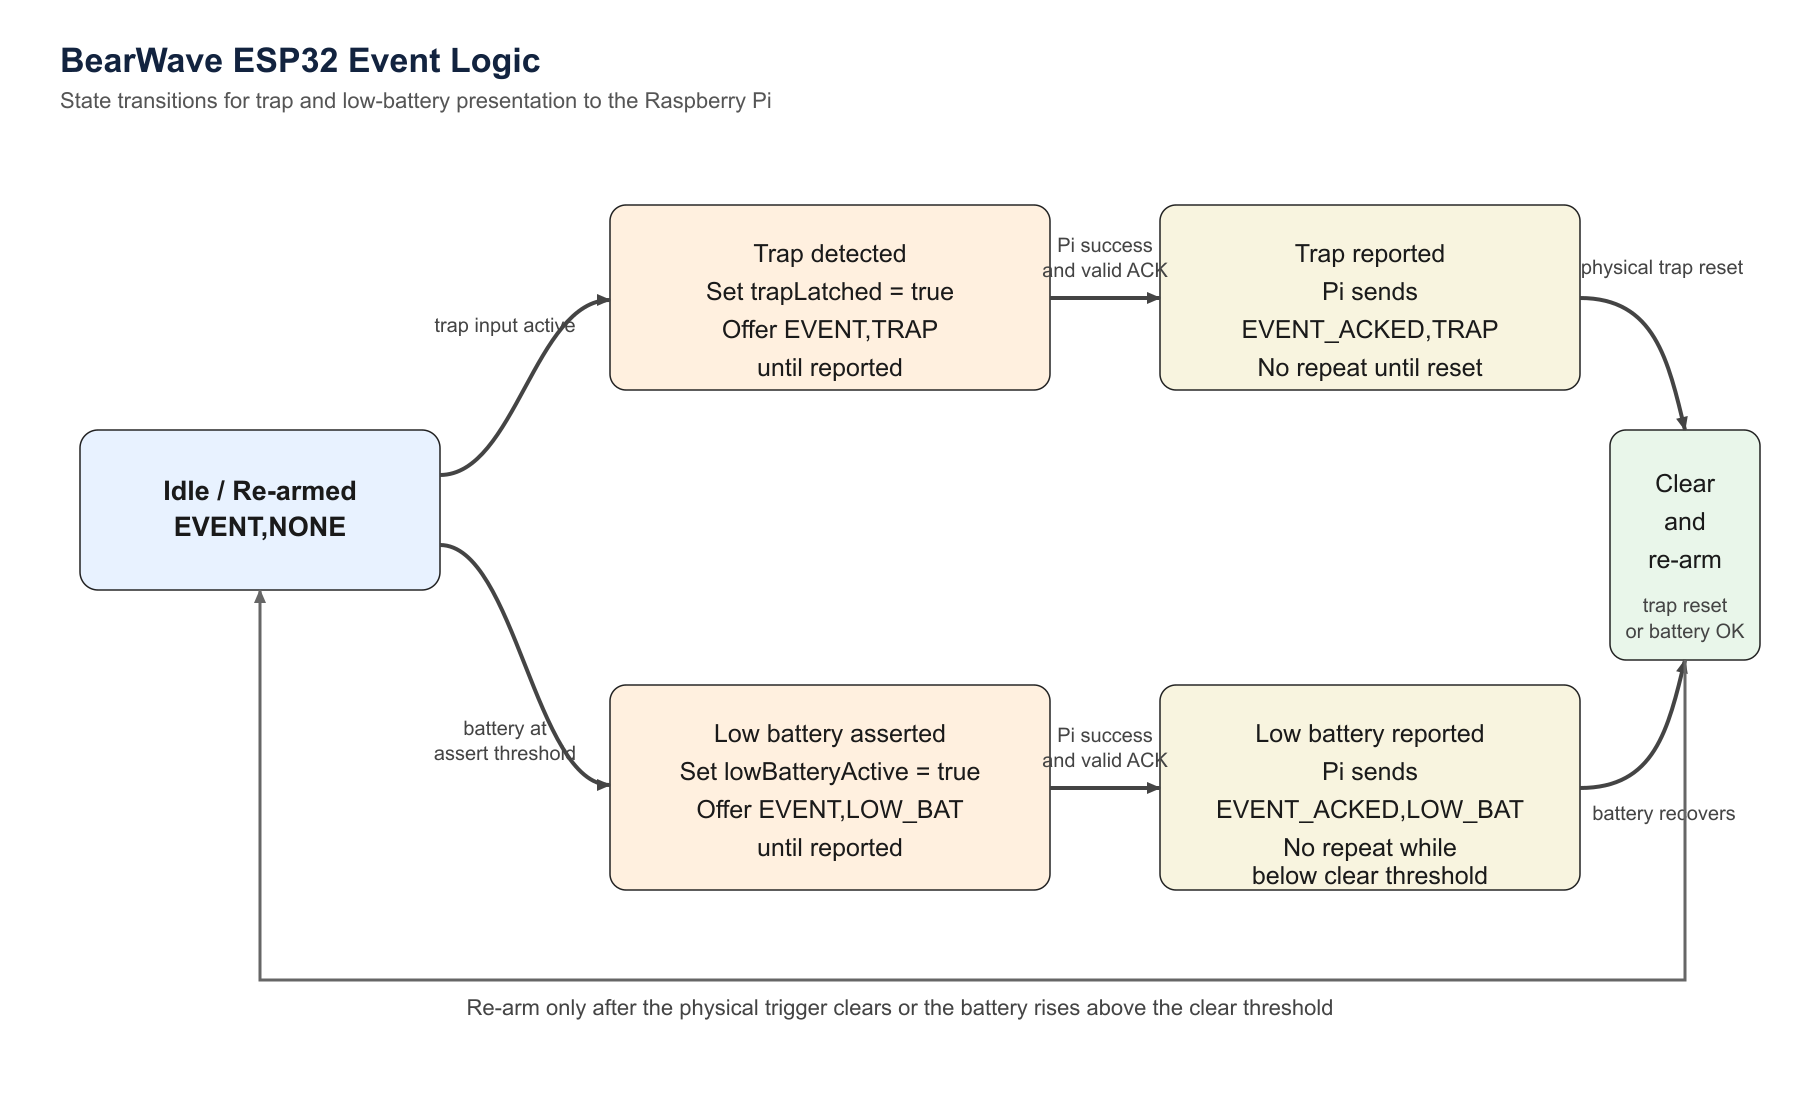
\includegraphics[width=0.95\linewidth]{images/bearwave_esp32_event_logic.png}
    \caption{Working ESP32 event-logic diagram showing how trap and low-battery conditions are latched, offered to the Raspberry Pi, suppressed after acknowledgement, and re-armed after the underlying condition clears.}
    \Description{State diagram for ESP32 event logic, showing idle and re-armed state, trap detected state, low-battery asserted state, reported states after acknowledgement, and condition-cleared return to idle.}
    \label{fig:esp32-event-logic}
\end{figure}

\subsubsection{Timing and Field Serviceability}
The firmware wake and heartbeat interval is user configurable rather than fixed by the hardware design. In the ESP32 supervisor sketch, the setting is the \texttt{WAKE\_INTERVAL\_US} constant in the \texttt{TEST SLEEP INTERVAL} configuration block, which is used to set the deep-sleep timer wake-up before the ESP32 powers down. The 15-minute value used in testing is therefore a bench-test setting, with 60 seconds available for rapid diagnostics. In a real field deployment the heartbeat interval would normally be configured to a much longer value, typically around four hours, depending on message urgency, battery capacity, and the acceptable maintenance interval. The Pi shutdown power-cut delay is 50 seconds, giving the Raspberry Pi time to complete Linux shutdown before the ESP32 removes rail power. These values are therefore treated as deployment-specific configuration parameters rather than universal constants: heartbeat interval, shutdown delay, and low-battery thresholds must be matched to the deployment battery, message urgency, and acceptable maintenance interval.

The Heltec OLED is retained as a local service display. This is not a core research contribution, but it is practically important because USB serial can back-feed the Raspberry Pi through 5 V during full power testing. The display provides immediate evidence of reset reason, wake reason, boot count, and rail state during bench and field diagnosis without requiring a laptop connection that may perturb the power system under test.

\subsection{Raspberry Pi Software Stack}
The Raspberry Pi Zero 2 W software provides the application-layer and radio-transport controller for the remote node. It is intentionally structured as a bounded wake-cycle program rather than as a continuously interactive application. On each wake cycle the Pi opens the UART link to the ESP32 supervisor, confirms that the hardware controller is alive, retrieves local state, connects to the local JS8Call API, selects the BearWave message to transmit, waits for a matching acknowledgement, optionally performs the SSTV still-image stage for acknowledged alarms, reports the outcome to the ESP32, and then requests managed shutdown.

This software layer preserves the architectural separation used throughout BearWave. The ESP32 is the hardware and event-state authority: it observes trap inputs, low-battery state, time/GPS information, and rail control. The Raspberry Pi is the application and radio-transport controller: it formats BearWave messages, interacts with JS8Call, handles acknowledgements, persists failed critical transmissions, and controls the optional alarm-image capture, encode, and transmit stage. This split keeps low-power supervision independent of the Linux-based communication stack and makes it possible to power the Pi down completely between reporting windows.

\begin{figure}[tbp]
    \centering
    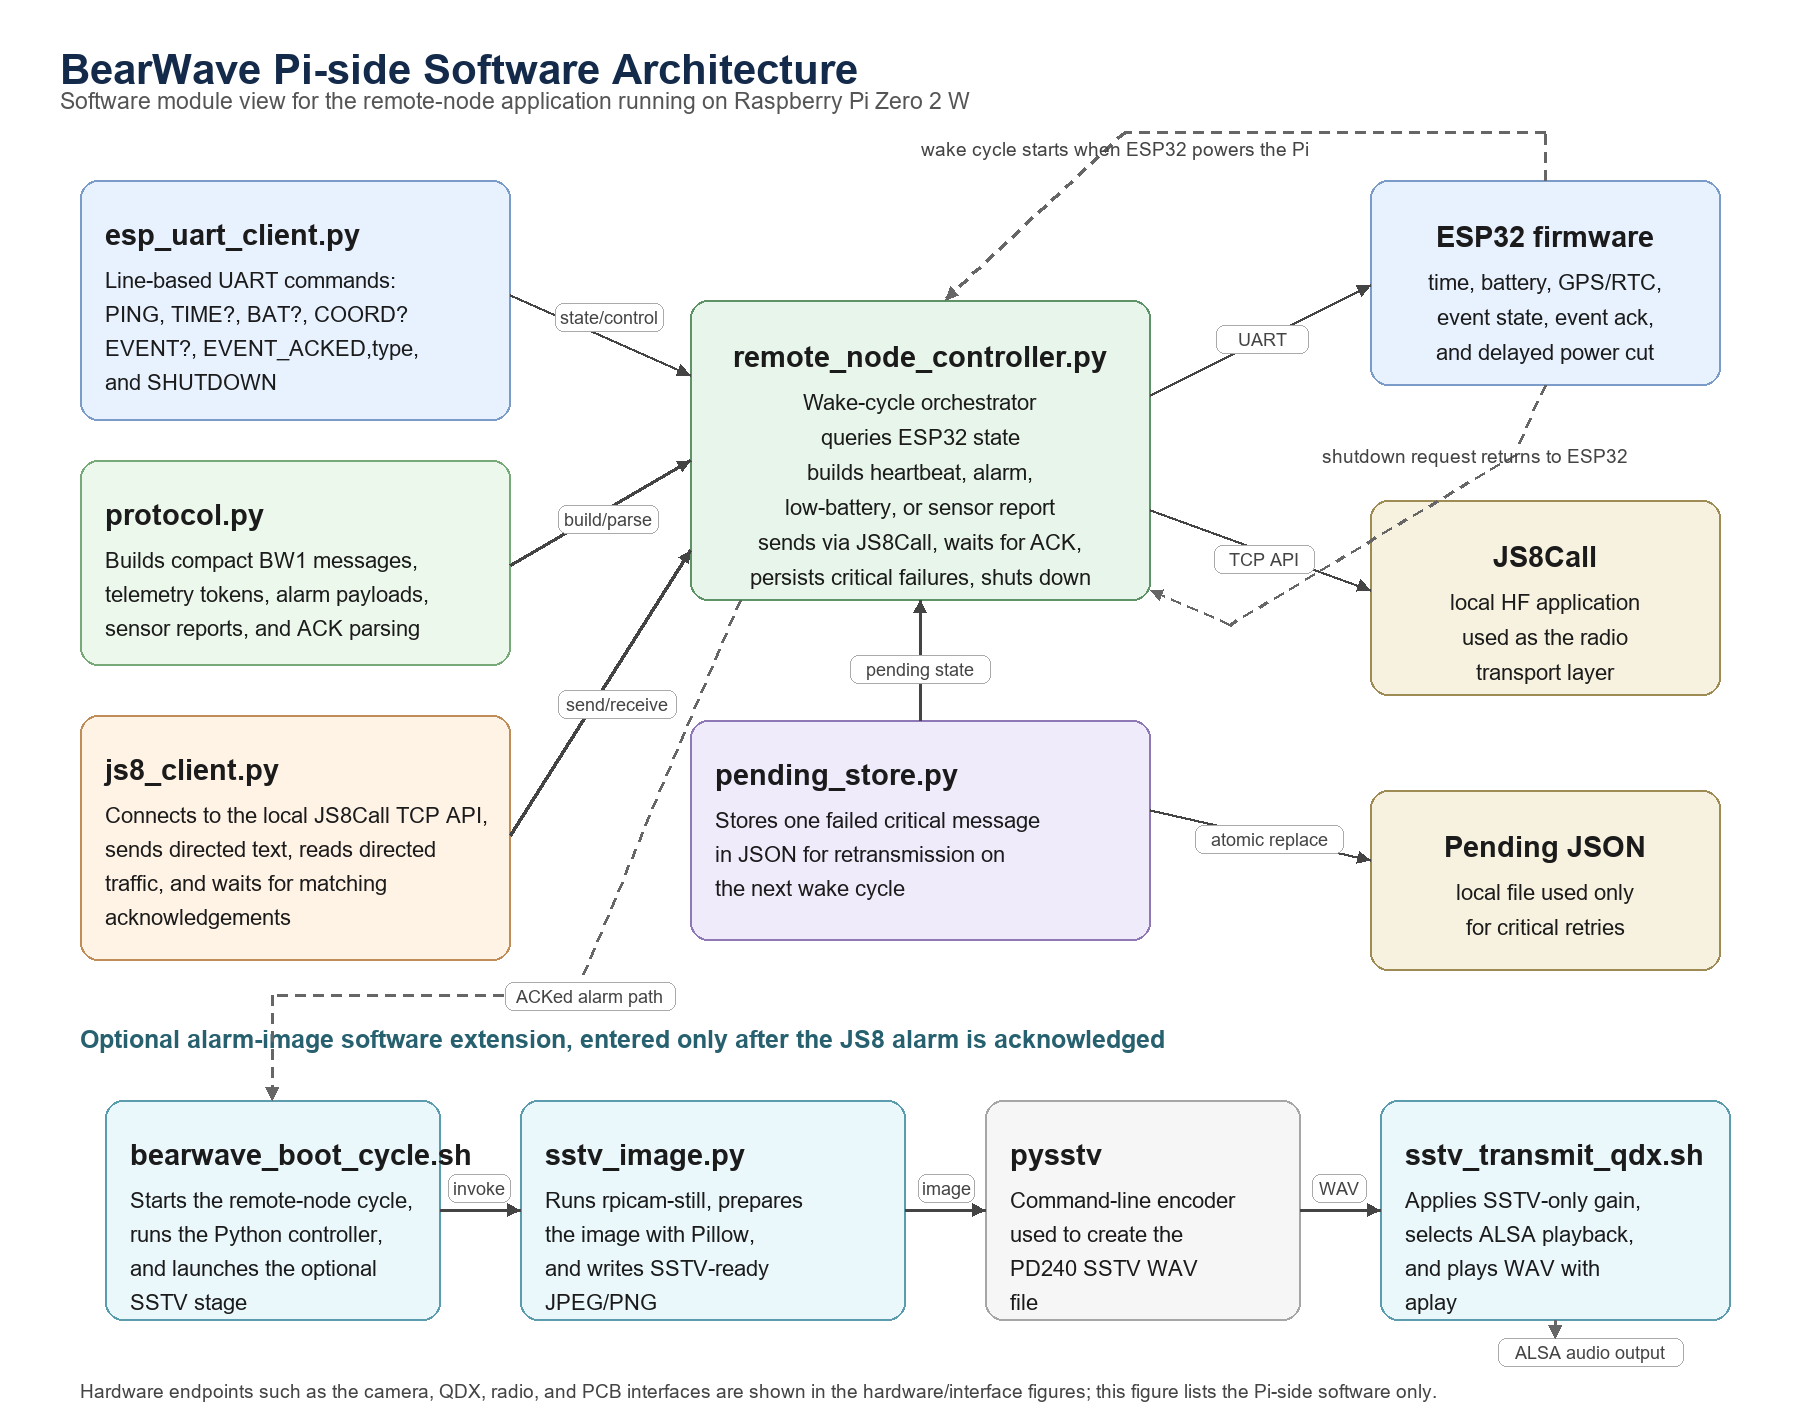
\includegraphics[width=0.95\linewidth]{images/bearwave_pi_software_architecture.png}
    \caption{Working Raspberry Pi remote-node software architecture showing the main Python modules, the ESP32 UART interface, the JS8Call transport interface, the SSTV image extension, and the pending-message store.}
    \Description{Module diagram showing the Raspberry Pi remote-node software. The primary BearWave path includes esp_uart_client.py for ESP32 UART commands, protocol.py for BW1 message construction and acknowledgement parsing, js8_client.py for the local JS8Call TCP API, pending_store.py for critical-message retry storage, remote_node_controller.py as the wake-cycle orchestrator, JS8Call as the compact text transport, the pending JSON file, and the ESP32 firmware. A secondary SSTV software branch is shown after an acknowledged alarm: bearwave_boot_cycle.sh invokes sstv_image.py, which runs rpicam-still and uses Pillow to prepare a still image; pysstv encodes a PD240 WAV; sstv_transmit_qdx.sh applies the SSTV transmit gain and plays the WAV with aplay through the selected ALSA output.}
    \label{fig:pi-software-architecture}
\end{figure}

\begin{table}[tbp]
\caption{Principal Raspberry Pi remote-node software modules.}
\label{tab:pi-software-modules}
\begin{tabularx}{\linewidth}{p{0.30\linewidth}X}
\toprule
Module & Responsibility \\
\midrule
\path{esp_uart_client.py} & Opens the Pi-to-ESP32 UART, sends line-based commands such as \texttt{PING}, \texttt{TIME?}, \texttt{BAT?}, \texttt{COORD?}, \texttt{EVENT?}, \texttt{EVENT\_ACKED,type}, and \texttt{SHUTDOWN}, and validates responses. \\
\path{protocol.py} & Builds compact \texttt{BW1} payloads for heartbeats, alarms, low-battery events, and \texttt{SR} sensor reports such as humidity or temperature; creates telemetry tokens; and parses acknowledgements. \\
\path{js8_client.py} & Connects to the local JS8Call TCP API, transmits directed text using JS8Call, receives asynchronous directed traffic, and waits for a matching acknowledgement. \\
\path{pending_store.py} & Stores one outstanding failed critical message in a JSON file so it can be retried on the next boot. Heartbeat failures are deliberately not persisted. \\
\path{remote_node_controller.py} & Coordinates the full wake cycle: state acquisition, message selection, retry logic, persistence, ESP32 event acknowledgement, and shutdown. \\
\path{bearwave_boot_cycle.sh} & Provides the appliance-style entry point for the Pi wake cycle, runs the Python controller, and launches the optional image stage only after an acknowledged alarm. \\
\path{sstv_image.py} & Runs the local camera capture command, prepares the alarm image using Pillow, applies SSTV mode-specific sizing, and writes the still image used by the encoder. \\
\texttt{rpicam-still} & Provides the command-line still-image capture interface used by the SSTV image-preparation script. \\
\texttt{Pillow} & Provides the Python image-processing functions used to crop, resize, and format captured images before SSTV encoding. \\
\texttt{pysstv} & Provides the command-line SSTV encoder used to convert the prepared still image into a PD240 audio waveform. \\
\path{sstv_transmit_qdx.sh} & Applies the SSTV-specific transmit gain, selects the configured ALSA playback path, and plays the generated waveform with \texttt{aplay}. \\
\texttt{aplay} & Provides the ALSA command-line playback utility used to send the SSTV waveform to the configured audio output. \\
\bottomrule
\end{tabularx}
\end{table}

At startup the controller validates the ESP32 link and retrieves the current state needed to construct a message. The first part of this state acquisition is a \texttt{TIME?} request to the ESP32 supervisor, which provides the RTC/GPS-derived UTC time required by the time-synchronised JS8Call modulation and by local log alignment. The controller then reads battery state, coordinates where available, and event state before connecting to JS8Call. It may also drain stale directed messages so that a delayed acknowledgement from an earlier attempt is not mistaken for the current reply. Before building a fresh heartbeat, alarm, or sensor report, the controller checks whether a critical message was persisted from a previous failed cycle. If such a pending message exists, it is transmitted before any newly observed routine heartbeat. This ordering prevents a trap or low-battery event from being hidden by a subsequent normal reporting cycle.

The persistence policy is intentionally asymmetric. Failed heartbeat transmissions are not written to disk because the next scheduled wake cycle will naturally produce another routine heartbeat. Failed critical messages are stored with enough metadata to reconstruct and retry the original application-layer message, including node identifier, message identifier, message type, flags, data field, creation time, latest attempt time, attempt count, and failure reason. The record is cleared only after the control node returns a valid acknowledgement matching both the expected node identifier and message identifier. This keeps field behaviour conservative without turning the remote node into a general-purpose message queue.

The SSTV extension is deliberately thin and is entered only after the compact alarm message has already been delivered and acknowledged. In the tested implementation the Pi captures a still image using the Raspberry Pi camera stack, prepares the image using Python/Pillow, encodes it to an SSTV audio waveform with \texttt{pysstv}, and plays the waveform through the QDX audio device. The current working configuration uses PD240 to favour image quality over transmission time. SSTV transmit gain is controlled separately from JS8Call transmit audio so that image transmission can be tuned without disturbing the primary alarm-message path.

\subsection{Wake, Transmit, and Shutdown Sequence}
The BearWave Linux setup is deliberately configured as a one-cycle remote-node appliance rather than as a continuously running workstation. When the ESP32 enables the Pi rail, Raspberry Pi OS boots on the Raspberry Pi Zero 2 W, exposes the ESP32 UART as \texttt{/dev/serial0}, starts the local JS8Call environment, and launches the BearWave Python entry point, \texttt{main.py}, from the remote-node software directory or virtual environment. The entry point loads environment-based configuration, including the ESP32 serial port and baud rate, JS8Call API host and port, control-node callsign, short BearWave node identifier, pending-message path, acknowledgement wait interval, retry count, stale-message drain setting, and combined-alarm policy. The JS8Call operating frequency is a user-defined radio configuration value rather than a fixed BearWave constant: 7.078 MHz was used as a bench/test setting, while earlier BearWave propagation trials indicate that operation around 5 MHz is likely to be more appropriate for the intended NVIS deployment scenario \cite{ButterworthMarkAndrew2025ERCi}. These Linux and radio-configuration details are part of the reproducible wake-cycle design because they affect boot time, service recovery, time synchronisation, and the interval before a message can be transmitted.

The nominal wake cycle links four software and hardware actors: the ESP32 supervisor, the Pi controller, JS8Call, and the control node. The ESP32 powers the Pi and exposes state over UART. The Pi first requests time from the ESP32 using \texttt{TIME?}; this is a critical step because JS8Call is a time-synchronised digital mode and incorrect system time can prevent reliable decoding or transmission scheduling. The Pi then queries battery state, coordinates where available, and current event state before sending the selected BearWave payload through JS8Call using the local TCP API. The control node reconstructs and validates the payload, updates its node-state model, and returns a compact directed acknowledgement. When the Pi receives a matching acknowledgement it can run the optional alarm-image stage, then reports critical-event delivery back to the ESP32 using \texttt{EVENT\_ACKED,type}, sends \texttt{SHUTDOWN}, and allows the ESP32 to remove Pi power after the configured shutdown interval.

\begin{figure}[tbp]
    \centering
    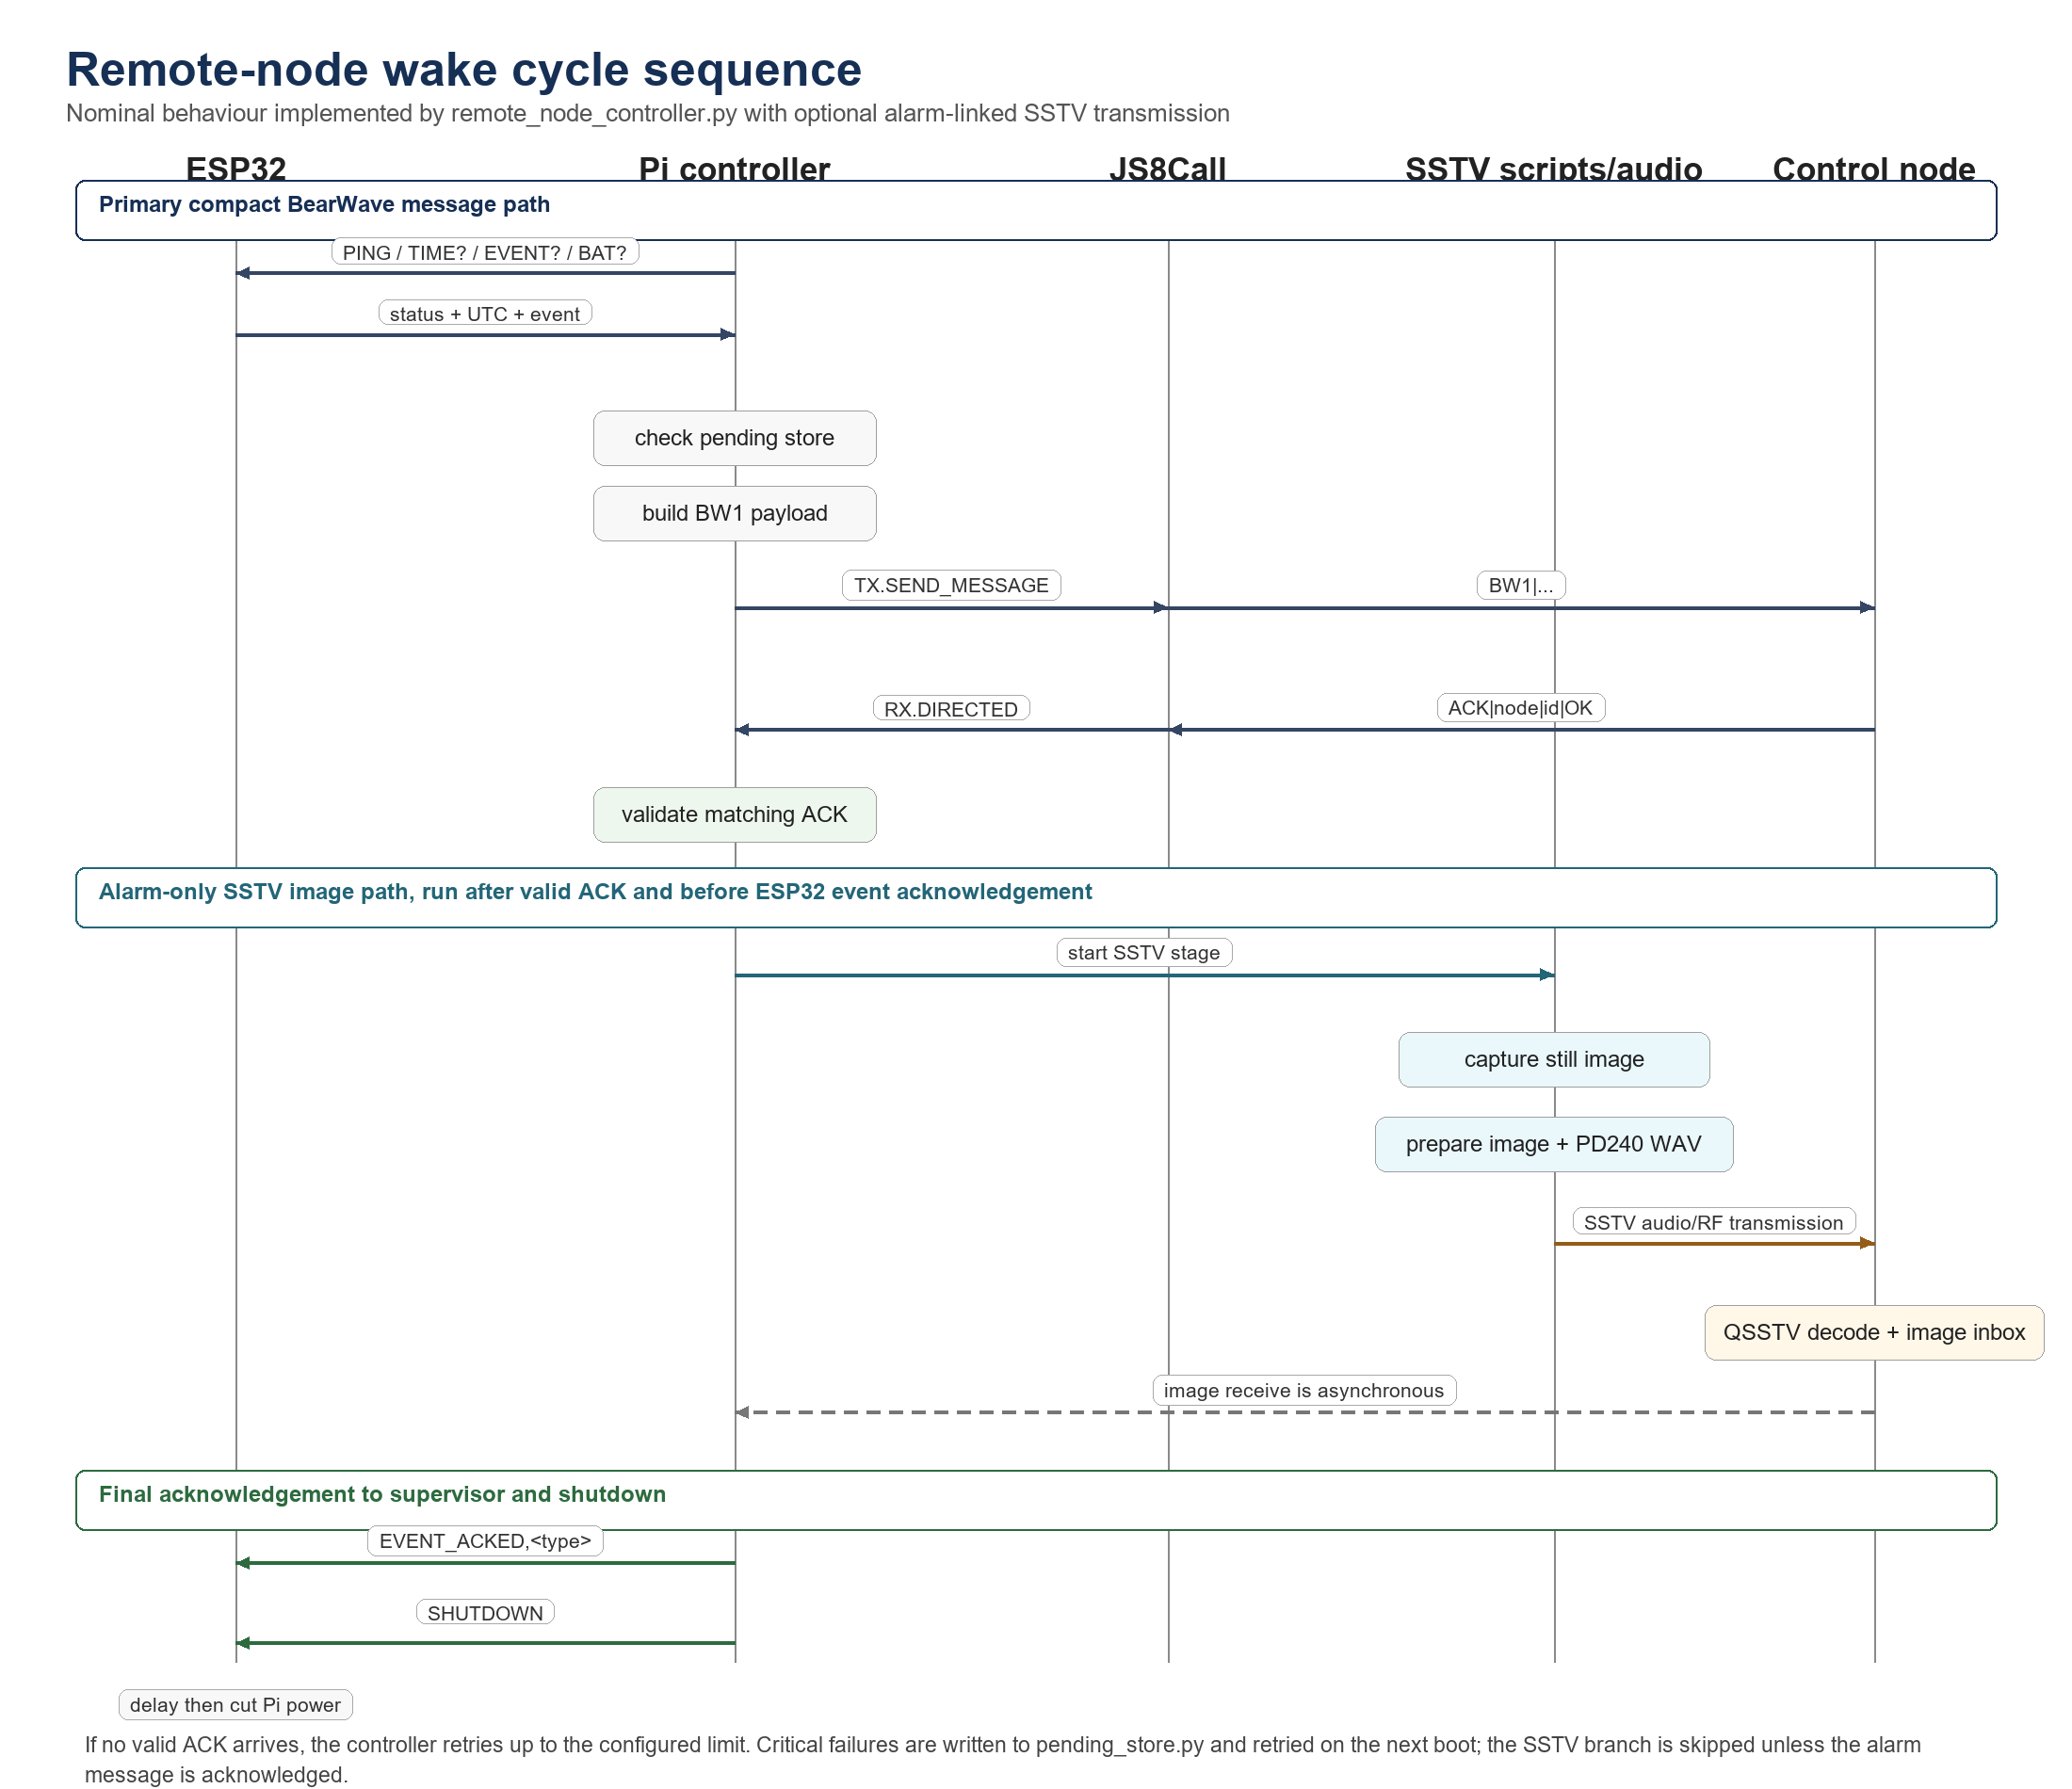
\includegraphics[width=0.95\linewidth]{images/bearwave_pi_wake_cycle_sequence.png}
    \caption{Nominal remote-node wake-cycle sequence implemented by the Raspberry Pi controller, showing the ESP32 time request, state acquisition, JS8Call transmission, acknowledgement handling, optional SSTV image transmission, event acknowledgement, and shutdown request.}
    \Description{Sequence diagram showing the Pi requesting time and event state from the ESP32, checking the pending store, building a BW1 payload, sending the message through JS8Call to the control node, and receiving a matching acknowledgement. For acknowledged alarm messages, an additional SSTV branch starts before the ESP32 event acknowledgement: the Pi starts the SSTV stage, captures a still image, prepares a PD240 WAV, transmits the SSTV audio/RF signal, and the control node decodes the image into its inbox. The Pi then sends EVENT_ACKED to the ESP32, requests shutdown, and the ESP32 cuts Pi power after a delay.}
    \label{fig:pi-wake-cycle-sequence}
\end{figure}

The controller decision flow is correspondingly simple. Pending critical messages take priority over newly built messages. If no pending critical message exists, the controller reads the current ESP32 event and telemetry state and builds the appropriate heartbeat, alarm, low-battery, or \texttt{SR} sensor-report payload. Transmission attempts are bounded by a configured acknowledgement wait interval and a maximum send-attempt count. In the current Raspberry Pi software this count defaults to three attempts per wake cycle, configured through \texttt{BEARWAVE\_MAX\_SEND\_ATTEMPTS}, and applies to heartbeat and alarm messages. If the acknowledgement is received, the controller clears any associated pending state, runs the optional SSTV stage for alarm cycles where enabled, and progresses to shutdown. If no acknowledgement arrives, only critical failures are persisted for retransmission at the next boot.

\begin{figure}[tbp]
    \centering
    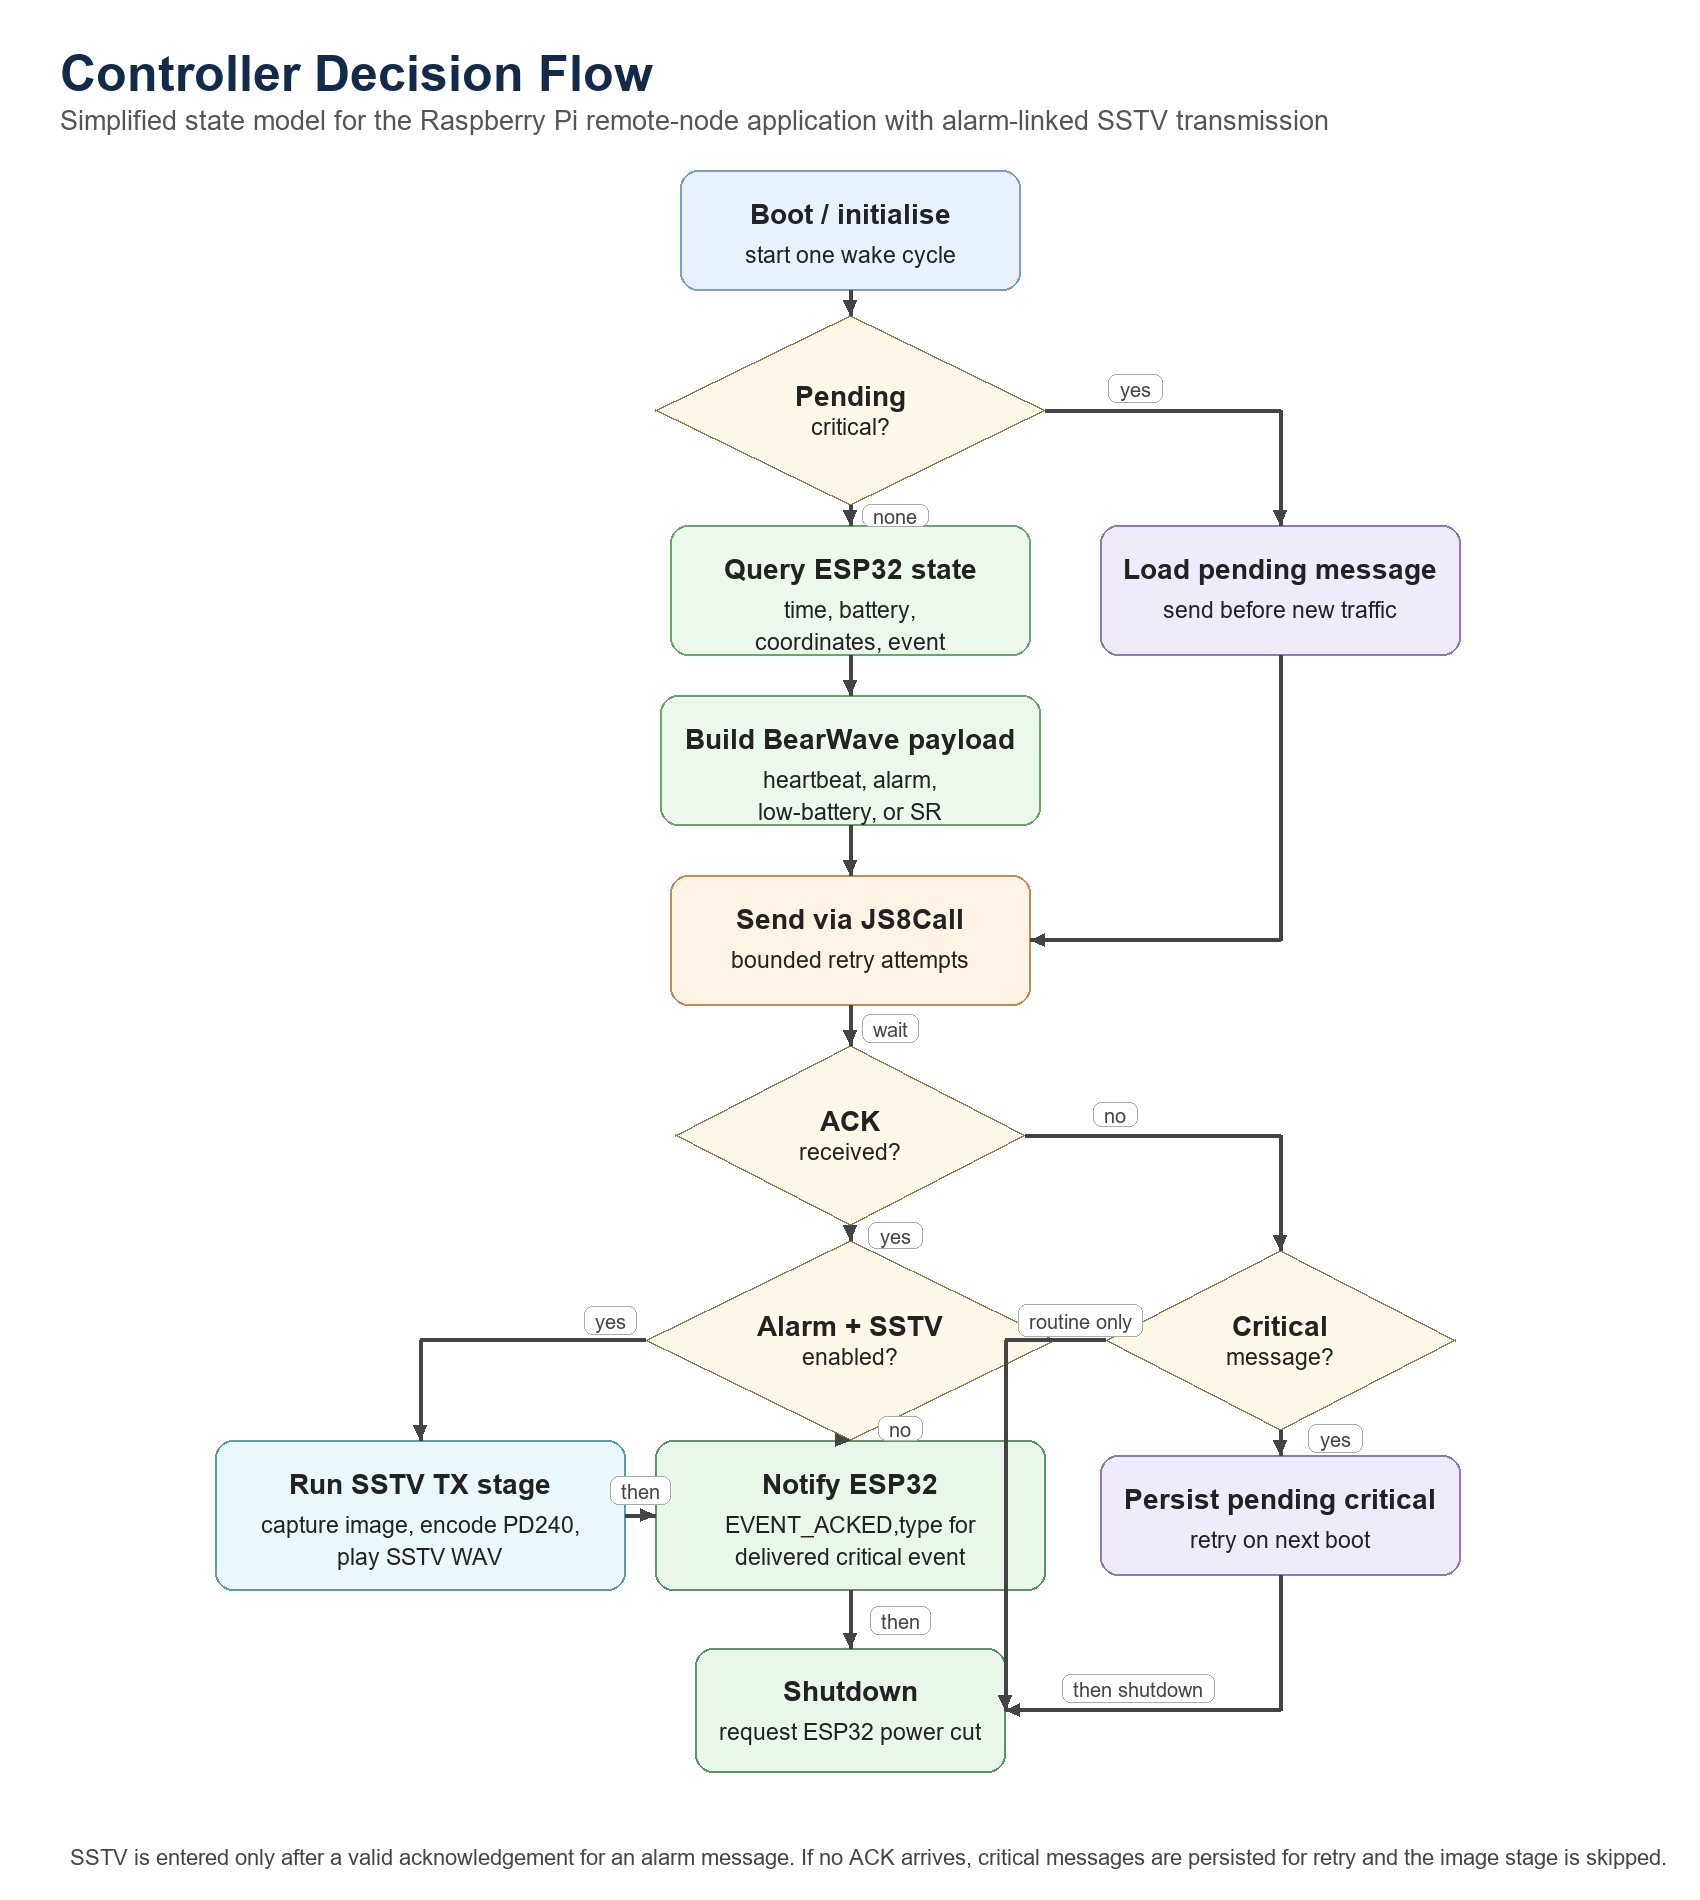
\includegraphics[width=0.95\linewidth]{images/bearwave_pi_controller_decision_flow.png}
    \caption{Working decision flow for the Raspberry Pi controller, showing pending critical-message priority, BearWave message construction, acknowledgement handling, optional SSTV transmission after acknowledged alarms, critical-message persistence, and shutdown.}
    \Description{Flow diagram showing boot, pending critical message check, ESP32 state query, heartbeat, alarm, or sensor-report construction, JS8Call send, and acknowledgement decision. If no acknowledgement is received, the controller checks whether the message is critical and either persists it for retry or shuts down. If a valid acknowledgement is received, the controller checks whether the delivered message is an alarm with SSTV enabled; if so, it runs the SSTV transmit stage to capture an image, encode PD240 audio, and play the SSTV waveform before notifying the ESP32. The successful path then sends EVENT_ACKED to the ESP32 and requests shutdown.}
    \label{fig:pi-controller-decision-flow}
\end{figure}

\begin{figure}[tbp]
    \centering
    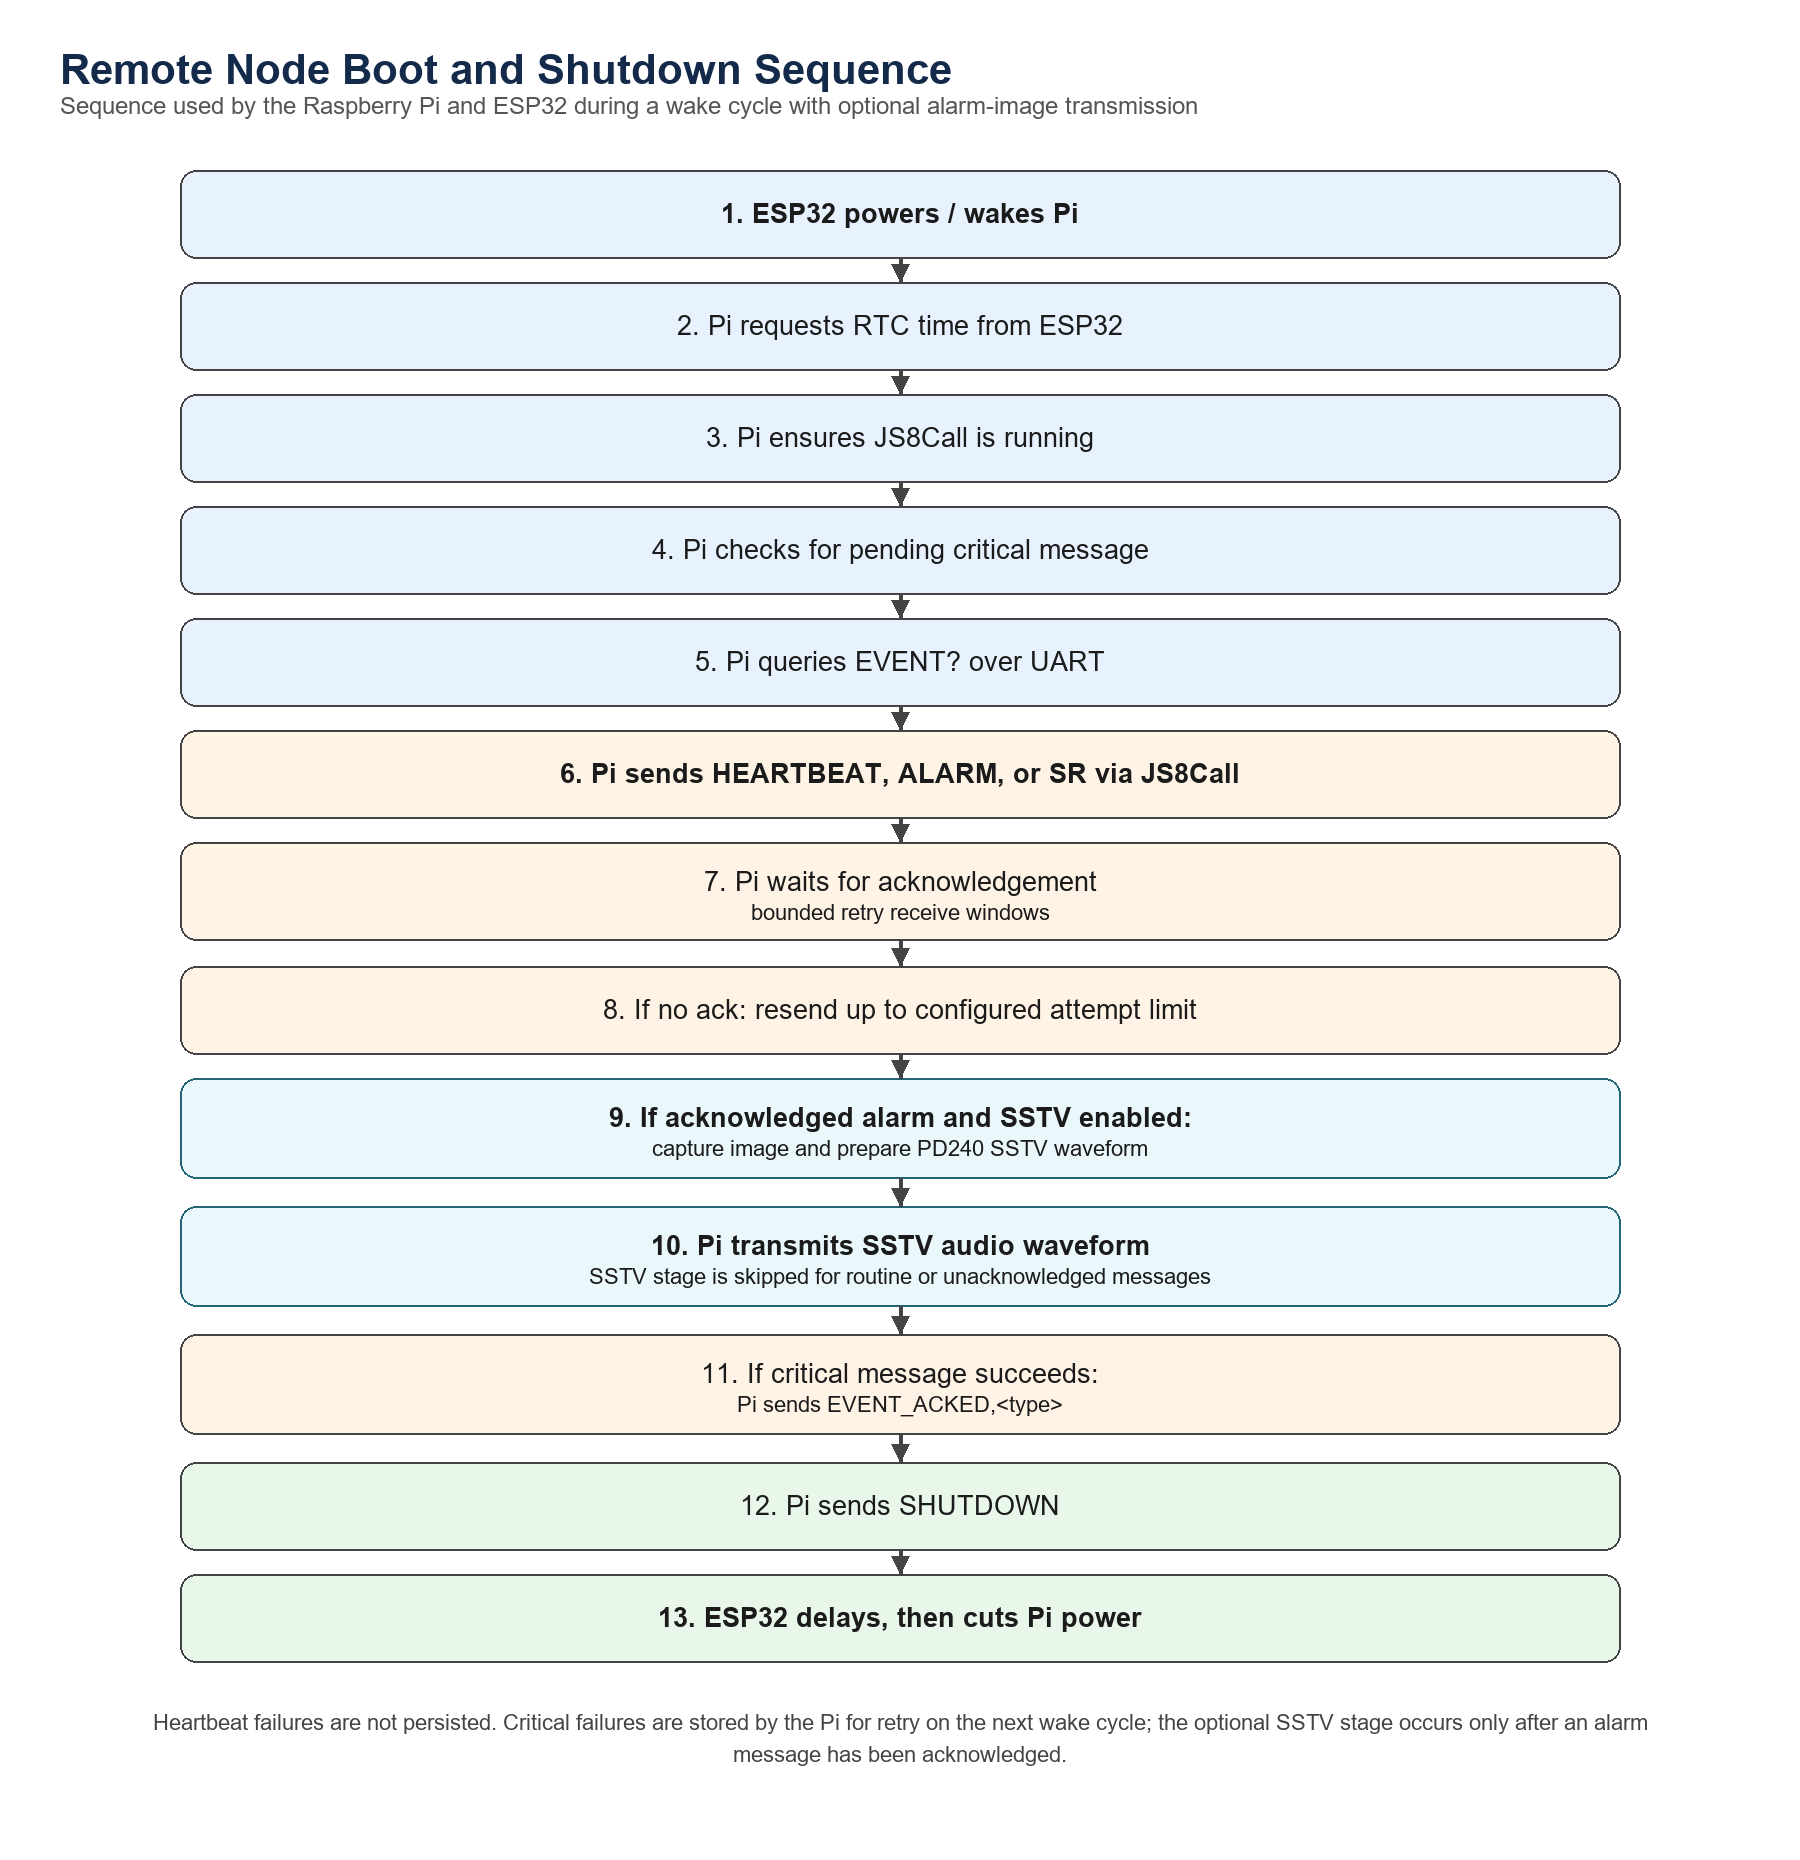
\includegraphics[width=0.88\linewidth]{images/bearwave_remote_node_boot_shutdown_sequence.png}
    \caption{Working remote-node boot and shutdown sequence showing the interaction between the ESP32 supervisor, Raspberry Pi, JS8Call transmission cycle, acknowledgement handling, optional SSTV image stage, and ESP32-controlled power removal.}
    \Description{Vertical flow diagram showing the ESP32 powering or waking the Raspberry Pi, the Pi requesting time, checking JS8Call and pending messages, querying events and telemetry, sending the selected BearWave payload, waiting for acknowledgement, and retrying if needed. For an acknowledged alarm with SSTV enabled, the Pi captures an image, prepares a PD240 SSTV waveform, and transmits the SSTV audio before sending EVENT_ACKED to the ESP32. The sequence then shows the Pi requesting shutdown and the ESP32 cutting Pi power after a delay.}
    \label{fig:remote-node-boot-shutdown}
\end{figure}

\subsection{Fault Handling and Recovery}
Fault handling in the Pi software is focused on preserving operationally important alarms while still allowing the node to complete its wake cycle. A failed heartbeat is treated as non-critical because another heartbeat will be generated at the next reporting interval. A failed trap or low-battery alarm is treated as critical and is persisted to local JSON storage for retransmission on the next boot. The persistence mechanism uses an atomic replace pattern so that a partially written file is less likely if power is removed during or shortly after the write.

\begin{table}[tbp]
\caption{Remote-node Pi fault-handling policy.}
\label{tab:pi-fault-policy}
\begin{tabularx}{\linewidth}{p{0.26\linewidth}X}
\toprule
Condition & Implemented or intended behaviour \\
\midrule
No matching acknowledgement & Retry up to the configured limit, currently three send attempts per wake cycle by default. Persist the failed message only if it is a critical trap or low-battery alarm. \\
Pending critical message on boot & Retransmit the pending message before building a new routine or event payload. Clear it only after a valid acknowledgement. \\
Stale directed traffic & Drain or ignore stale JS8Call directed messages so that an acknowledgement from a previous transmission is not matched to the current message. \\
ESP32 event acknowledged & Send \texttt{EVENT\_ACKED,type} to the ESP32 after successful critical delivery so the supervisor can suppress repeat presentation until the condition clears. \\
End of cycle & Send \texttt{SHUTDOWN} to the ESP32 and rely on the supervisor's delayed power-cut sequence to remove Pi power. \\
\bottomrule
\end{tabularx}
\end{table}

This policy avoids presenting diagnostic code as the research contribution while still documenting the reliability behaviour that matters in the field. The central claim is that the remote node distinguishes routine loss from critical alarm loss: ordinary heartbeat failures are allowed to be superseded by the next scheduled heartbeat, while failed alarms are carried across a power cycle until the control node confirms receipt.

\section{Message Format and Communication Protocol}
The protocol description below reflects the current ESP32, Raspberry Pi, and control-node code. This alignment is important because the protocol is the shared contract between all three software layers.

\subsection{Protocol Overview}
BearWave uses a compact application-layer protocol carried inside JS8Call messages to support communication between power-constrained remote nodes and a permanently listening control node. The protocol is designed for brief wake-transmit-listen cycles, where the remote node is intended to complete transmission and acknowledgement within a single 15-second JS8Call phase whenever channel conditions allow. This design keeps the higher-power Raspberry Pi and radio path active only for the period required to report an event or heartbeat, while preserving a deterministic method for confirming that a specific message was received.

The protocol supports four immediate operational needs: routine heartbeats, directly wired trap alarms, LoRa sensor alarms, and low-battery alarms. It is also extensible so that ESP32-local or LoRa-attached sensors can contribute compact telemetry values and alarm states, such as temperature, humidity, PIR activity, contact state, or equipment-health alarms, without requiring a redesign of the message envelope or the remote-node PCB.

The SSTV image extension is intentionally outside the compact BearWave protocol envelope. The \texttt{BW1} message remains the authoritative alarm and acknowledgement record; the image is a secondary analogue still-image transmission associated with that event by timing and by the control-node image watcher. This design avoids adding binary image data, file transfer state, or long identifiers to the primary alarm message while still allowing an operator to inspect visual evidence when the link supports it.

\subsection{Scalability and Intended Deployment Size}
BearWave is not a single-node protocol. Each message carries a compact node identifier, and the control-node software maintains state per remote node, allowing the same base station to receive, log, display, and acknowledge messages from multiple field units. Where the JS8Call receive path can decode multiple transmissions in the same monitoring period, the BearWave parser can separate them by node identifier and message identifier. In protocol terms, the address space and message structure support a substantially larger network than the expected initial deployment; in the present configuration this capacity is on the order of hundreds of nodes, approximately 200.

This theoretical capacity is not the operational target. BearWave is designed for small conservation deployments where staff can realistically install, inspect, power, and respond to the monitored assets. The intended scale for the present system is approximately ten trap-monitoring points per control node. This is large enough to reduce routine inspection effort and demonstrate multi-node operation, while remaining manageable in terms of field servicing, dashboard readability, acknowledgement timing, RF contention, and response workload. Larger deployments would require explicit planning around node scheduling, alarm rate, operator workflow, and maintenance logistics rather than only a larger node-number range.

\begin{table}[tbp]
\centering
\caption{BearWave application-layer protocol requirements.}
\label{tab:protocol-requirements}
\begin{tabularx}{\textwidth}{p{0.28\textwidth}X}
\toprule
Requirement & Rationale \\
\midrule
Compactness & The message body is kept as short as practical in order to minimise airtime and improve reliability under weak-signal conditions. \\
Deterministic acknowledgement & Every transmission contains a compact unique identifier so that the control node can acknowledge a specific message unambiguously. \\
Extensibility & The format admits additional sensor and alarm payloads without changing the core grammar. \\
Machine parsing with human readability & The format remains simple for software to parse while remaining readable during development, field testing, and troubleshooting. \\
Economy of addressing & Long callsigns remain in the JS8Call addressing layer and are not repeated unnecessarily inside the application payload. \\
\bottomrule
\end{tabularx}
\end{table}

\subsection{Protocol Envelope}
The BearWave message envelope is defined as a fixed, compact field structure with a flexible data segment:

\begin{center}
\texttt{BW1\textbar{}\(\langle\)node\(\rangle\)\textbar{}\(\langle\)type\(\rangle\)\textbar{}\(\langle\)id\(\rangle\)\textbar{}\(\langle\)flags\(\rangle\)\textbar{}\(\langle\)data\(\rangle\)}
\end{center}

\begin{figure}[tbp]
    \centering
    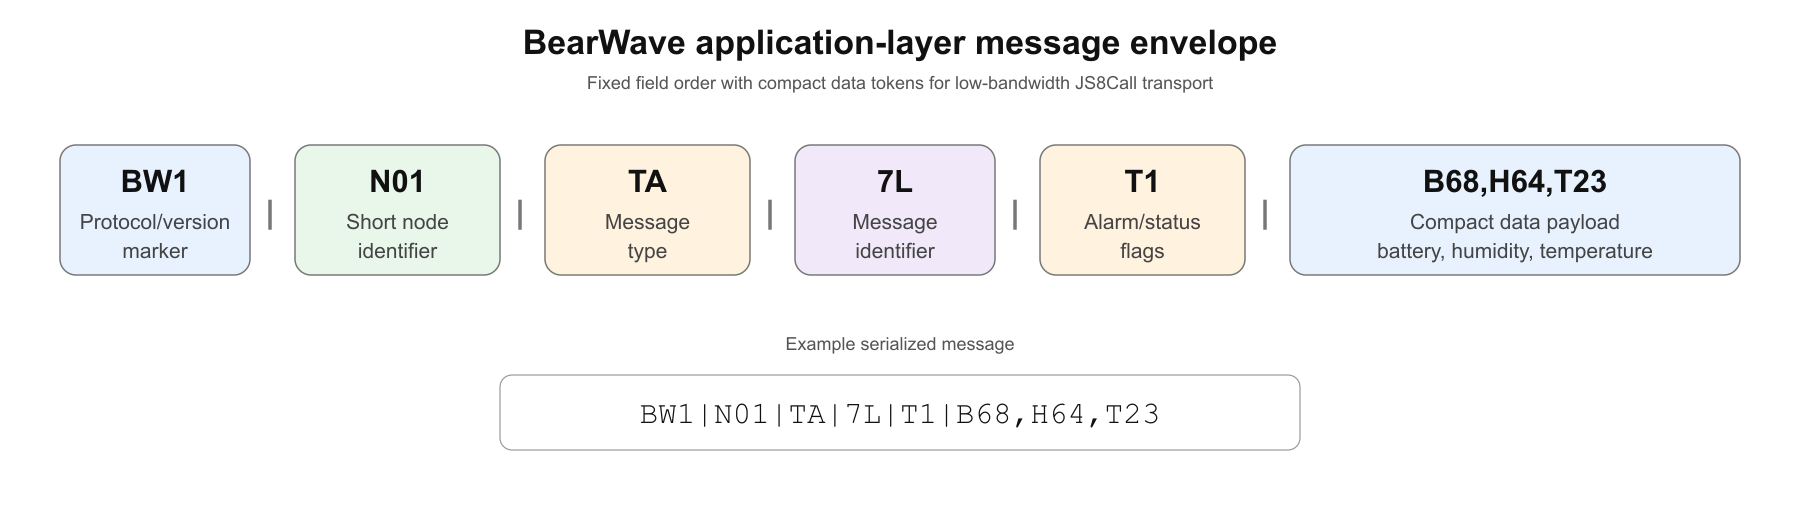
\includegraphics[width=0.95\linewidth]{images/bearwave_message_envelope.png}
    \caption{BearWave application-layer message envelope showing the fixed protocol fields and compact telemetry payload.}
    \Description{Diagram showing a BearWave message split into protocol version, node identifier, message type, message identifier, flags, and compact data payload.}
    \label{fig:message-envelope}
\end{figure}

\begin{table}[tbp]
\centering
\caption{BearWave message-envelope field definitions.}
\label{tab:message-fields}
\begin{tabularx}{\textwidth}{p{0.16\textwidth}p{0.22\textwidth}X}
\toprule
Field & Meaning & Description \\
\midrule
\texttt{BW1} & Protocol/version marker & Identifies BearWave Protocol Version 1 and provides room for future protocol evolution. \\
\(\langle\)\texttt{node}\(\rangle\) & Short node ID & A compact internal identifier such as \texttt{N01} or \texttt{N02}. This avoids repeating long callsigns already carried by JS8Call. \\
\(\langle\)\texttt{type}\(\rangle\) & Message class & Identifies heartbeat, alarm, low battery, sensor report, or fault message types. \\
\(\langle\)\texttt{id}\(\rangle\) & Message identifier & A short unique reference used for acknowledgement matching and retransmission control. \\
\(\langle\)\texttt{flags}\(\rangle\) & Alarm/status flags & A compact summary of active event state such as trap asserted or low battery active. \\
\(\langle\)\texttt{data}\(\rangle\) & Compact telemetry fields & A comma-separated list of short key-value elements carrying battery level and optional sensor values. \\
\bottomrule
\end{tabularx}
\end{table}

\subsection{Message Classes and Telemetry Keys}
Message classes are intentionally short two-character codes. These codes keep the message readable during field testing while avoiding the airtime and parsing overhead of verbose labels.

\begin{table}[tbp]
\centering
\caption{BearWave message type definitions.}
\label{tab:message-types}
\begin{tabularx}{\textwidth}{p{0.15\textwidth}p{0.22\textwidth}X}
\toprule
Code & Meaning & Purpose \\
\midrule
\texttt{HB} & Heartbeat & Routine wake-up and check-in message. \\
\texttt{TA} & Trap or sensor alarm & Critical wired-trap, LoRa-sensor, or other alarm event requiring acknowledgement. \\
\texttt{LB} & Low battery & Battery condition has crossed a low-power threshold. \\
\texttt{SR} & Sensor report & Additional telemetry values such as temperature or humidity. \\
\texttt{FT} & Fault report & System or subsystem fault condition. \\
\bottomrule
\end{tabularx}
\end{table}

Telemetry values are encoded using short key prefixes to preserve payload space. The same grammar can therefore carry fixed alarm messages, LoRa sensor alarm states, and richer multi-sensor reports.

\begin{table}[tbp]
\centering
\caption{Compact sensor and status key registry for BearWave Protocol Version 1.}
\label{tab:sensor-key-registry}
\begin{tabularx}{\textwidth}{p{0.12\textwidth}p{0.30\textwidth}p{0.16\textwidth}X}
\toprule
Key & Meaning & Example & Interpretation \\
\midrule
\texttt{B} & Battery percentage & \texttt{B72} & Battery at 72\%. \\
\texttt{V} & Battery voltage, tenths of a volt & \texttt{V118} & Battery at 11.8 V. \\
\texttt{T} & Temperature & \texttt{T23} & Temperature 23 \(^{\circ}\)C. \\
\texttt{H} & Humidity & \texttt{H64} & Relative humidity 64\%. \\
\texttt{P} & PIR state & \texttt{P1} & PIR active. \\
\texttt{R} & Reed/contact state & \texttt{R1} & Contact active. \\
\texttt{L} & Light level & \texttt{L44} & Encoded light level. \\
\texttt{X} & Fault code & \texttt{X03} & Fault code 03. \\
\bottomrule
\end{tabularx}
\end{table}

\begin{table}[tbp]
\centering
\caption{Example BearWave operational messages.}
\label{tab:operational-message-examples}
\small
\begin{tabularx}{\textwidth}{p{0.20\textwidth}p{0.35\textwidth}X}
\toprule
Message class & Encoded example & Interpretation \\
\midrule
Heartbeat & \texttt{BW1\textbar N01\textbar HB\textbar 7K\textbar 0\textbar B72} & Node \texttt{N01} routine heartbeat with battery at 72\%. \\
Trap alarm & \texttt{BW1\textbar N01\textbar TA\textbar 7L\textbar T1\textbar B68} & Node \texttt{N01} trap alarm with trap asserted and battery at 68\%. \\
Low battery alarm & \texttt{BW1\textbar N01\textbar LB\textbar 7M\textbar L1\textbar B18} & Node \texttt{N01} low-battery event with battery at 18\%. \\
Extended sensor report & \texttt{BW1\textbar N01\textbar SR\textbar 7N\textbar 0\textbar B71,H64,T23} & Illustrative future report carrying battery, humidity, and temperature values. \\
\bottomrule
\end{tabularx}
\end{table}

\subsection{Acknowledgement Protocol}
Reliable delivery requires the control node to acknowledge a specific message rather than issue a generic response. In the current control-node code, the acknowledgement is transmitted as a compact directed JS8Call payload containing the acknowledgement marker, originating node identifier, and original message identifier:

\begin{center}
\texttt{A\textbar{}\(\langle\)node\(\rangle\)\textbar{}\(\langle\)id\(\rangle\)}
\end{center}

\begin{figure}[tbp]
    \centering
    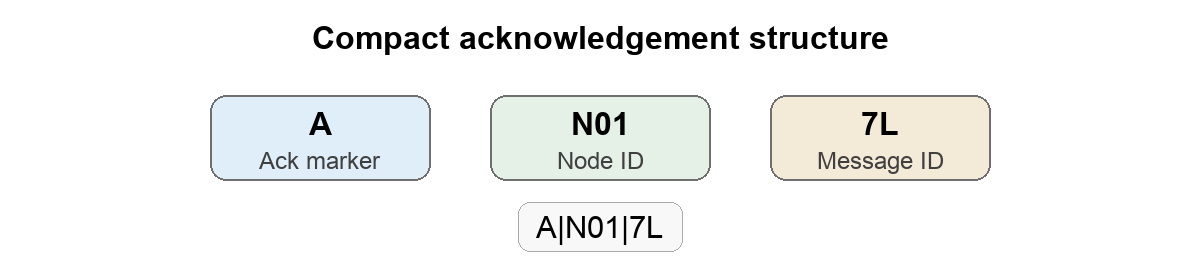
\includegraphics[width=0.85\linewidth]{images/bearwave_ack_structure.png}
    \caption{Compact acknowledgement structure used by the control node to confirm receipt of a specific message.}
    \Description{Diagram showing a compact acknowledgement message split into acknowledgement marker, node identifier, and message identifier.}
    \label{fig:ack-structure}
\end{figure}

\begin{table}[tbp]
\centering
\caption{BearWave acknowledgement field definitions.}
\label{tab:ack-fields}
\begin{tabularx}{\textwidth}{p{0.18\textwidth}p{0.18\textwidth}X}
\toprule
Field & Example & Description \\
\midrule
\texttt{A} & \texttt{A} & Compact acknowledgement marker used by the current control-node code. \\
\(\langle\)\texttt{node}\(\rangle\) & \texttt{N01} & Node whose message is being acknowledged. \\
\(\langle\)\texttt{id}\(\rangle\) & \texttt{7L} & Message identifier being confirmed. \\
\bottomrule
\end{tabularx}
\end{table}

\subsection{Rationale and Encoding Constraints}
A compact tagged encoding was selected in preference to verbose formats such as JSON or XML because every additional character increases airtime on the HF link. Under weak-signal conditions, a shorter transmission improves robustness and reduces the probability that the remote node will need to remain awake for multiple send-retry cycles. The design also leaves addressing economy to the JS8Call layer: long callsigns are already present in the radio-addressing context and do not need to be repeated inside every application payload.

Routine operational messages omit a full timestamp. This is a deliberate trade-off: the control node can timestamp receipt locally, while the remote node can retain richer timing information in its own logs. The over-the-air message is therefore reserved for the fields that matter most during transmission: node identity, event class, message identifier, status flags, and compact telemetry.

LoRa connectivity is treated as a local ingress mechanism rather than as the long-haul BearWave link. The Heltec supervisor can remain available while the Raspberry Pi and HF radio chain are off, allowing nearby LoRa-connected sensors to send directly addressed packets to the remote node. When such a packet is received, the Heltec firmware can wake or service the LoRa receive event, check that the packet is addressed to the node, normalise the sensor value into the local event, alarm, or telemetry state, and expose it to the Raspberry Pi during the next BearWave wake cycle. The LoRa packet is therefore not forwarded verbatim over HF; it is converted into compact BearWave data fields that preserve the short message envelope.

\begin{table}[tbp]
\centering
\caption{Illustrative comparison between compact BearWave encoding and a JSON-style equivalent.}
\label{tab:encoding-comparison}
\begin{tabularx}{\textwidth}{p{0.24\textwidth}p{0.28\textwidth}X}
\toprule
Format & Example & Practical implication \\
\midrule
BearWave tagged format & \texttt{BW1\textbar N01\textbar TA\textbar 7L\textbar T1\textbar B68} & Short, field-ordered, readable during field testing, and easy to match with a compact acknowledgement. \\
JSON-style equivalent & \begin{tabular}[t]{@{}l@{}}\texttt{\{"node":"N01",}\\\texttt{"type":"TA",}\\\texttt{"id":"7L",}\\\texttt{"trap":1,}\\\texttt{"battery":68\}}\end{tabular} & More self-describing but much longer, increasing airtime and parser complexity for no immediate field benefit. \\
\bottomrule
\end{tabularx}
\end{table}

\subsection{Operational Role Within the BearWave Node}
Within the remote node, the ESP32 acts as the hardware and event-status authority, while the Raspberry Pi acts as the radio and application-layer controller. The Pi queries the ESP32 for time, battery state, and event condition; constructs the BearWave protocol payload; transmits via JS8Call; and waits for a matching acknowledgement from the control node. Once the acknowledgement is received, the Pi reports the outcome back to the ESP32, allowing the supervisory firmware to mark the event as acknowledged and return the node to its low-power state.

\begin{figure}[tbp]
    \centering
    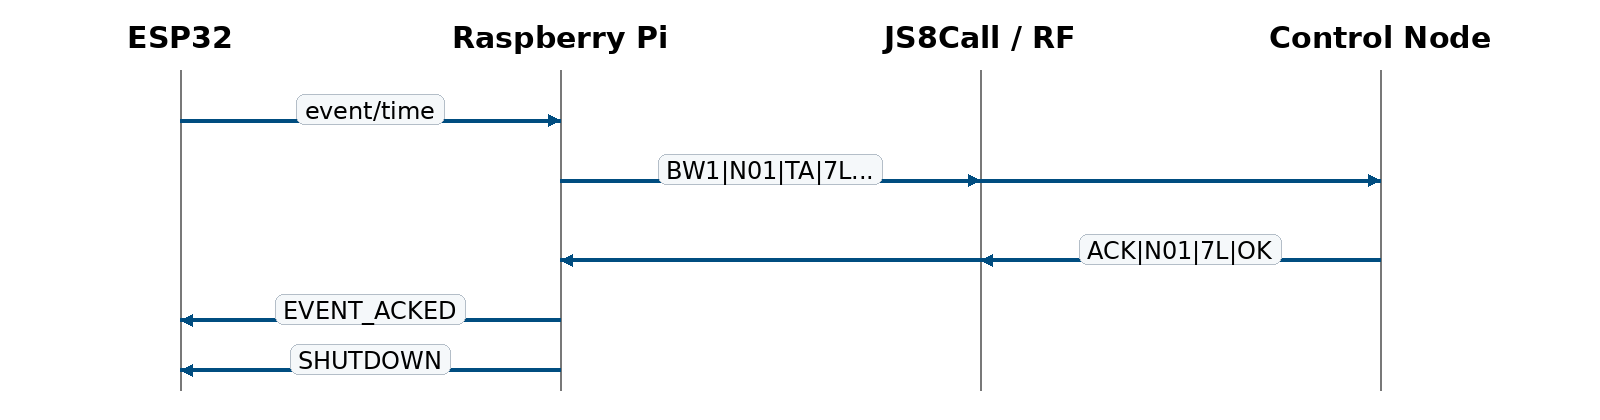
\includegraphics[width=0.95\linewidth]{images/bearwave_message_exchange_workflow.png}
    \caption{Remote-node message exchange workflow from ESP32 state acquisition to control-node acknowledgement, optional alarm-linked SSTV image transmission, and shutdown.}
    \Description{Sequence diagram showing an ESP32 passing event and time state to the Raspberry Pi, the Pi transmitting a BearWave message through JS8Call and RF, the control node returning an acknowledgement, and the Pi reporting acknowledged state and shutdown to the ESP32.}
    \label{fig:message-exchange-workflow}
\end{figure}

\subsection{Extensibility, Verification, and Future Registry}
The protocol remains extensible because the outer envelope stays fixed while the \(\langle\)\texttt{data}\(\rangle\) field can carry additional short-form sensor elements. This allows LoRa-attached sensor alarms, LoRa telemetry, or ESP32-local measurements to be represented without redesigning the parser or the control-node acknowledgement process. In practical terms, the protocol can scale from simple heartbeat and alarm messages to local sensor alarms and richer environmental telemetry while preserving the same field order, message grammar, and acknowledgement logic.

The protocol is verified through bench tests before field deployment. These tests include message-length checks, parser round-trip tests, acknowledgement matching trials, malformed-message rejection, and send-wait-retry behaviour for unacknowledged critical messages. A formal sensor-key registry is maintained as an appendix or repository file so that future additions remain consistent across firmware, Raspberry Pi software, and control-node parsing code.

The SSTV image extension does not require a new BearWave message type or sensor-key entry because the image is not carried inside the \texttt{BW1} payload. Instead, the compact alarm message and acknowledgement remain the authoritative protocol exchange, while SSTV mode, transmit-gain setting, decode success, and thumbnail association are treated as system-level configuration and validation items.

The retransmission policy is intentionally conservative. The current Raspberry Pi controller defaults to three send attempts per wake cycle, set by \texttt{BEARWAVE\_MAX\_SEND\_ATTEMPTS}. The acknowledgement wait defaults to 90 seconds per attempt and is set by \nolinkurl{BEARWAVE_ACK_WAIT_PER_ATTEMPT_S}. The control node currently schedules acknowledgements after 4000 ms and suppresses duplicate acknowledgement scheduling for the same node/message pair for 120000 ms. Routine heartbeats may be superseded by the next scheduled heartbeat, but failed critical alarms are retained by the Pi-side pending-message store and retried before newly generated routine traffic. A pending critical message is cleared only when a matching acknowledgement confirms the expected node identifier and message identifier.

\section{Build, Validation, and Deployment Workflow}
The build workflow is an essential part of the BearWave contribution. The system is open and locally maintainable, so this final report describes not only the circuit and code but also the practical route from design files to a working node. This section therefore follows the same logic as open ecological hardware reports: it identifies the released artefacts, describes assembly order, defines software installation steps, and specifies bench checks that a node passes before it is taken to the field.

\subsection{Design Files and Bill of Materials}
The reproducible release is made available through the BearWave Paper 3 GitHub repository \cite{BearWaveRepository}. The repository includes the design files and software artefacts required to audit and reproduce the system. For the remote node, these include PCB source files, schematic, Gerbers, bill-of-materials information, STL files for 3D printing, SolidWorks CAD files, assembly notes, ESP32 firmware, Raspberry Pi scripts, SSTV capture/encode/transmit scripts, configuration templates, and test payloads. For the control node, they include the Node.js service, dashboard files, image-watcher code, JS8Call configuration notes, SparkSDR/QSSTV audio-routing notes, Hermes Lite SDR setup notes, example node-to-callsign mapping, and logging configuration.

The bill of materials separates the remote node and control node because their cost drivers are different. The remote node includes the PCB, Heltec ESP32, Raspberry Pi Zero 2 W, GPS, RTC, power components, QDX, modified ATU100, battery hardware, connectors, and enclosure. The control node includes the Raspberry Pi 4, touch display, Hermes Lite SDR, antenna materials, storage, and power supply. Publishing these as separate BOMs helps conservation users decide whether to build a single trial link, a base station plus multiple field nodes, or only the field hardware for integration with an existing station.

\subsection{Remote Node Assembly}
Remote-node assembly proceeds from low-risk electrical checks to full system integration. The PCB is first inspected visually, then tested for shorts on the main battery input, protected battery rail, 5 V rail, 12 V rail, and 3.3 V logic paths before any expensive modules are inserted. Power-protection and regulator behaviour are verified using a current-limited bench supply. Only after the rails have been checked are the Heltec ESP32, Raspberry Pi, GPS, RTC, and external radio hardware connected.

The next stage is interface assembly. Trap inputs, battery-sense wiring, UART connections, and rail-status lines are checked using simple firmware tests before the Pi communication stack is introduced. The QDX and modified ATU100 are then integrated with the Pi and inverted-V dipole path, confirming that the radio chain can be powered, recognised, tuned, and returned to a low-power state. Final inspection records connector polarity, fuse values, antenna routing, enclosure cable exits, and any service labels needed by field staff.

\subsection{Software Deployment and Configuration}
The software deployment is part of the reproducibility record because BearWave depends on coordinated behaviour across three targets. The ESP32 is flashed with the supervisory firmware and configured with wake interval, battery thresholds, GPIO assignments, UART settings, and deployment-specific identifiers. The Raspberry Pi remote node is prepared with Python 3, the BearWave remote-node controller, access to \texttt{/dev/serial0}, JS8Call, QDX/radio interface configuration, camera access, Pillow, \texttt{pysstv}, a user-defined JS8Call frequency setting, pending-message storage path, node identifier, SSTV mode and gain settings, and control-node addressing information. The JS8Call frequency is deployment configuration rather than a fixed BearWave constant: the 7.078 MHz value used during testing is not the expected operational setting, and a 5 MHz configuration is likely to follow from the earlier BearWave trials. The control node is prepared with Node.js dependencies, JS8Call API access, Hermes Lite SDR configuration, SparkSDR/QSSTV audio routing, image-inbox path, dashboard/kiosk service startup, log paths, acknowledgement delay, duplicate-suppression window, and node-to-callsign mappings.

A repeatable post-deployment sanity test links installation to validation. The ESP32 responds to \texttt{PING}, \texttt{TIME?}, \texttt{BAT?}, and \texttt{EVENT?}. The Pi queries the ESP32, builds a known BearWave payload, and hands it to JS8Call. The control node receives a known payload, reconstructs it if fragmented, updates node state, logs the event, and schedules the expected acknowledgement. Where the SSTV extension is enabled, a non-transmit dependency check confirms camera capture, image conversion, SSTV encoding, and audio playback, followed by a controlled receive test that places a decoded image in the control-node inbox and displays it on the dashboard. These checks demonstrate that the firmware, remote-node controller, JS8Call transport, SSTV image path, and control-node software share the same protocol assumptions before formal bench validation begins.

\subsection{Bench Validation}
\begin{table}[tbp]
\centering
\caption{Validation checklist for a newly assembled BearWave remote node.}
\label{tab:validation-checklist}
\begin{tabularx}{\textwidth}{p{0.25\textwidth}p{0.25\textwidth}X}
\toprule
Test & Expected result & Evidence recorded \\
\midrule
Protected battery input & Correct polarity and protected battery rail present & Multimeter reading, visual inspection \\
5 V rail latch & Rail turns on/off by button and \texttt{ENABLE5VPULSE} firmware input & Voltage log, LED/status output \\
12 V rail latch & Rail turns on/off by button and \texttt{ENABLE12VPULSE} firmware input & Voltage log, load test \\
RTC operation & Time retained after main power removal & Serial log, timestamp check \\
Trap input & GPIO changes state reliably on switch activation & Firmware log, repeated trigger count \\
Battery ADC & Reported voltage matches measured voltage within tolerance & Calibration record \\
Pi wake & Pi boots when 5 V rail is enabled & Boot log, current profile \\
Message transmit & Known test message reaches control node & Control-node log entry \\
SSTV image path & Alarm-linked image is captured, encoded, transmitted, decoded, and displayed & Remote image/WAV files, control-node image inbox entry, and dashboard thumbnail \\
\bottomrule
\end{tabularx}
\end{table}

\subsection{Field Deployment Procedure}
Field deployment is treated as a controlled commissioning process rather than as simple placement of a box. The site is chosen for sensor relevance, safe access, and a workable inverted-V dipole arrangement. The enclosure is mounted where it is protected from standing water and mechanical disturbance while still allowing battery service and cable inspection. Sensor wiring is strain-relieved and labelled, and antenna/feedline exits are protected against water ingress.

After connection, the installer performs an initial heartbeat test and confirms that the control node records the correct node identifier, message type, battery value, and timestamp. A trap-input test is then performed where ethically and operationally appropriate. The deployment record includes site identifier, antenna geometry, battery capacity, node ID, firmware version, control-node mapping, first successful heartbeat, first successful alarm test, and planned service interval.

\section{Evaluation and Characterisation Methodology}
The evaluation is designed to test the complete BearWave system rather than only the HF link. The central question is whether a physical event can be detected, preserved, transmitted, logged, acknowledged, optionally followed by a received still image, and followed by a controlled return to low power. The methodology therefore combines electrical characterisation, functional event testing, latency measurement, communication trials, image-path checks, and operating-lifetime modelling.

\subsection{Power Characterisation}
Power characterisation measures current in each major operating state: ESP32 idle supervision, ESP32 with display active, GPS active, RTC-backed sleep, Pi boot, Pi idle, JS8Call preparation, HF transmit through the QDX, receive/acknowledgement wait, SSTV capture/encode/playback and SSTV transmit through the QDX, ATU100 tuning, and shutdown delay. These values are measured at the battery input where possible so that regulator losses are included. The resulting profile supports lifetime estimates under heartbeat-only, low-alarm, moderate-alarm, and stress scenarios.

\subsection{Functional Event Tests}
Functional tests verify that physical and software events produce the expected state transitions. Wired trap inputs are triggered repeatedly to confirm detection, latching, acknowledgement-based suppression, and re-arm after the underlying condition clears. Low-battery behaviour is tested around the assert and clear thresholds to verify hysteresis. If local wireless ingress is used, LoRa-attached or other secondary sensors are tested separately from the HF path so that local acquisition failures are not confused with long-haul communication failures.

\subsection{Latency Tests}
Alarm-to-alert latency is decomposed into observable stages: physical trigger, ESP32 detection, event latch, rail enable, Pi boot, ESP32 state query, message construction, JS8Call scheduling, transmission duration, control-node decode, dashboard update, acknowledgement scheduling, acknowledgement reception, optional camera capture, SSTV encoding, SSTV transmission, QSSTV decode, thumbnail update, ESP32 event acknowledgement, and shutdown. Reporting these stages separately is more useful than a single end-to-end number because it shows where delay and energy are introduced. The JS8 alarm is still the primary alert and arrives before the image stage; SSTV adds visual evidence at the cost of additional airtime and energy. This does not imply that Raspberry Pi boot time is operationally problematic: in the intended conservation setting, workers may be several hours from a trap, so a boot interval on the order of 30 seconds is insignificant compared with field response time. The boot interval and image interval are therefore reported for reproducibility, power modelling, and comparison with future implementations rather than as limiting factors in alarm response.

\subsection{Communication Tests}
Communication evaluation distinguishes previous BearWave propagation results from new tests of the integrated node. Earlier work justifies HF/NVIS as the communication approach, while Paper 3 reports system-level message behaviour: heartbeat delivery, alarm delivery, acknowledgement success, duplicate suppression, retry outcomes, malformed-message rejection, SSTV image delivery and decode, clickable-thumbnail display, and completeness of control-node logs. The evaluation treats alarm-message delivery and acknowledgement as the primary success criterion. SSTV image reception is reported separately as best-effort visual evidence because a failed or partial image decode does not invalidate an already acknowledged alarm. Trials include controlled bench tests using known payloads and outdoor link tests using the actual QDX, modified ATU100, inverted-V dipole, Hermes Lite SDR, SparkSDR, JS8Call, and QSSTV configuration.

\subsection{Operational Scenario Modelling}
Operational modelling converts measured current and timing values into deployment expectations. The model includes battery capacity, heartbeat interval, alarm rate, retry probability, Pi boot time, JS8 transmit duration, acknowledgement wait, tuner activity, optional camera capture and SSTV transmit duration, regulator efficiency, and sleep current. At minimum, the paper compares heartbeat-only monitoring, alarm operation without image transfer, alarm operation with image transfer, moderate alarm traffic, and a stress case with repeated retries. This makes clear how energy use changes as the system moves from routine monitoring to an event-heavy period.

The characterisation record separates the integrated-system evidence in this paper from the earlier propagation results. For Paper 3, the relevant evidence is whether the released hardware, firmware, Raspberry Pi software, control-node software, message protocol, and optional image path operate together as a reproducible monitoring system. The key outputs are therefore rail behaviour, event latching, wake--transmit--image--shutdown sequencing, acknowledgement handling, duplicate suppression, malformed-message rejection, image decode/display behaviour, build practicality, and power assumptions that support deployment-lifetime estimates. Long-duration unattended rainforest deployment remains future work rather than a result claimed here.

\section{Discussion}
The discussion interprets BearWave as an integration contribution. The individual technologies are not novel in isolation: Raspberry Pis, ESP32 modules, JS8Call, QRP transceivers, SDRs, and dipoles are all established tools. The contribution is the way they are arranged into a low-duty-cycle, open, reproducible system for conservation monitoring.

\subsection{From Communication Link to Deployable Conservation System}
The main advance from the earlier BearWave work is the transition from demonstrating a communication link to documenting a deployable system. A radio link alone does not solve the field problem: the system must detect events, preserve them while high-power components are off, wake the Pi and radio reliably, encode a short message, deliver it to a base station, acknowledge it when required, optionally add visual evidence, log it, display it, and shut down safely. The deployable-system claim rests on the reliable alarm-message and acknowledgement path; successful SSTV reception is valuable supporting evidence, but the alarm remains valid even if the image path fails. Paper 3 therefore contributes the architecture and reproducibility layer that allows the communication result to become a practical conservation tool.

\subsection{Relationship to Earlier BearWave Papers}
\begin{table}[tbp]
\centering
\caption{Positioning of Paper 3 relative to the earlier BearWave work.}
\label{tab:paper-positioning}
\begin{tabularx}{\textwidth}{p{0.18\textwidth}p{0.26\textwidth}X}
\toprule
Paper & Main focus & Role in PhD arc \\
\midrule
Paper 1 \cite{ButterworthMarkAndrew2025ERCi} & Conservation problem and communication requirement & Establishes why remote monitoring is needed and what constraints matter. \\
Paper 2 \cite{Butterworth2026BorneoFieldTrial} & HF/NVIS BearWave communication feasibility & Demonstrates that low-power NVIS can carry low-bandwidth alerts in challenging non-line-of-sight settings. \\
Paper 3 & Complete open hardware/software monitoring system & Documents the buildable system that turns the communication concept into a conservation tool. \\
\bottomrule
\end{tabularx}
\end{table}

\subsection{Comparison with Alternative Architectures}
An always-on Raspberry Pi architecture would simplify software but would be poorly matched to long unattended deployment because the highest-load subsystem would remain powered continuously. A LoRa-only architecture would reduce remote-node energy use, but would require gateways or relay infrastructure that may not exist across the required area \cite{Augustin2016LoRa}. Satellite messengers reduce dependence on terrestrial infrastructure but introduce recurring cost, sky-view constraints, and limited local adaptability. Commercial trap-monitoring systems already demonstrate demand for remote trap alerts: examples include satellite trapsite transmitters from Telonics and Vectronic, and cellular smart-trap systems such as OcuTrap \cite{TelonicsTrapsiteTransmitters,VectronicTT5,OcuTrapSmartWildlifeTraps}. These products may be operationally mature, but they are often closed systems with limited repairability, dependence on subscription or cellular/satellite service availability, and less freedom to adapt message formats or sensors.

BearWave accepts a different set of trade-offs. It is narrowband, slower, and more operationally specialised than many alternatives, but it gives conservation users a buildable path for long-haul low-bandwidth alerts where terrestrial infrastructure is weak. The SSTV extension reinforces this trade-off: the alarm remains a short, acknowledged text message, while an image is added only when the value of visual verification justifies several minutes of additional transmission. The reliable low-power alarm path is therefore the core contribution; SSTV is an opportunistic evidence layer whose reception cannot be guaranteed under all propagation, audio-level, or interference conditions. Its value is strongest when message volume is low, event importance is high, and local maintainability matters.

\subsection{Open Hardware and Local Adoption}
For conservation organisations, local adoption depends on more than technical performance. Systems must be affordable, repairable, understandable, and adaptable to local field practice. Open hardware and open software allow users to replace connectors, alter enclosures, add sensors, change message keys, and diagnose faults without waiting for a vendor-controlled product cycle. This is especially important in under-resourced settings where shipping delays, import costs, and proprietary repair processes can prevent equipment from being useful when it is most needed.

BearWave is therefore documented as infrastructure rather than as a sealed instrument. Publishing the PCB files, STL files for 3D printing, SolidWorks CAD files, firmware, Pi software, control-node software, message format, and validation workflow supports training, local repair, and future adaptation.

\subsection{Generalisability}
Although the immediate motivation comes from conservation monitoring and trap-alert scenarios, the system is not limited to one species or sensor. The same architecture could carry camera-trap health reports, intrusion alerts, flood warnings, equipment-health beacons, microclimate summaries, or field-station safety messages. The common requirement is a low-data-rate event or status message from a remote location to a fixed monitoring point. Future versions can extend the compact sensor-key registry while preserving the same envelope and acknowledgement logic.

This wider relevance is consistent with work on communications for infrastructure-limited and disaster-prone settings. Long-distance Wi-Fi telemedicine deployments in the Peruvian Amazon demonstrate the need for locally maintainable communication systems in rural and developing-region contexts \cite{Telemedicine}. VHF/HF emergency data links between hospitals in isolated disaster-prone areas, and studies of NVIS for emergency and disaster medicine, show that low-bandwidth radio links remain relevant where conventional infrastructure is absent, damaged, or operationally fragile \cite{Performance,Subekti2003NVIS}. International emergency-communication planning similarly recognises the need for regionally harmonised spectrum and resilient radio services during disaster relief \cite{ITU_EmergencyBands}. BearWave is not presented as a disaster-response system, but its design principles--local sensing, low-power operation, store-and-retry messaging, compact payloads, and independence from terrestrial backhaul--align with the requirements identified in disaster monitoring and remote-area sensing literature \cite{Disaster,Antarctica}.

\section{Limitations and Future Work}
Several limitations bound the contribution. First, the enclosure and final ruggedisation are still under development. The electronics, firmware, software, and message protocol can be evaluated on the bench and in controlled outdoor tests, but long-term rainforest deployment will also depend on moisture control, cable exits, insects, mechanical strain, battery access, and antenna routing. Second, the final integrated hardware has not yet undergone extended unattended rainforest deployment, so the paper distinguishes validated bench or local field behaviour from future long-duration rainforest trials.

Third, BearWave is deliberately low bandwidth. The core protocol is text-first and is not intended for broadband imagery, audio streams, video, or high-rate telemetry. The SSTV extension transmits a single low-resolution still image after an alarm, using a slow secondary analogue path rather than carrying image data inside the compact message protocol. This is useful for visual verification, but it is best-effort: it adds airtime, energy use, and decode sensitivity, and image reception is not guaranteed even when the alarm message has been delivered correctly. It complements rather than replaces camera traps, acoustic loggers, or broadband telemetry systems. Fourth, HF/NVIS performance remains dependent on frequency selection, ionospheric conditions, antenna installation, regulatory constraints, operator competence, and receive/transmit audio levels. The inverted-V dipole arrangement and audio chain must therefore be documented as part of the system, not as removable details.

Fifth, Raspberry Pi boot time is treated primarily as part of the energy and duty-cycle budget rather than as a real-time reporting constraint. BearWave alarms are intended for very remote conservation systems, where the operational value is reliable delivery without repeated site visits rather than urgent minute-by-minute response. The evaluation therefore reports boot and message-cycle timing for reproducibility, lifetime modelling, and comparison with future implementations, while avoiding claims that the system provides real-time alarm notification.

Future work addresses three main extensions. The first is a secure message protocol. The present protocol prioritises compactness, deterministic parsing, acknowledgement behaviour, and field readability, but deployments involving anti-poaching activity, animal locations, or sensitive site information require authentication, encryption, replay protection, and a practical key-management workflow. In these environments, security is not only a confidentiality requirement: unauthenticated messages could create false trap alerts, hide genuine alarms, or imitate acknowledgements and control responses. A future protocol version should therefore support authenticated encryption, or at minimum a keyed message authentication code, so that the remote and control nodes can reject forged, replayed, or modified traffic. This must be designed carefully because cryptographic metadata increases message length, and BearWave's HF link is intentionally narrowband.

The second extension is stronger image handling. The current prototype implements the first stage: alarm-triggered still-image transmission by SSTV and local display as a clickable control-node thumbnail. Future work should add explicit image receipt state, image quality assessment, selective image modes, better camera mounting and exposure control, and clearer handling for failed or partial decodes. A future alarm-image mode could also use higher transmit power or a more conservative image mode than the routine low-power message path, because an alarm that requires a field visit will normally lead to battery inspection or replacement when the trap is attended and the animal is released. BearWave does not attempt to carry video over the HF/NVIS channel, but stored local media could still be correlated with the same event identifier when intermittent cellular, Wi-Fi, LoRa gateway, or manual service access is available.

The third extension is stronger bidirectionality. The present return path is deliberately limited to acknowledgement messages, which keeps the protocol simple and reduces the risk of unintended remote action. A future control-message layer could extend acknowledgements with authenticated operator commands, including a remote trap-release option where the hardware supports safe actuation. Such a feature would require explicit animal-welfare safeguards, local fail-safe behaviour, command authentication, audit logging, confirmation of operator intent, and deployment-specific approval before it could be treated as part of the operational system.

\section{Conclusion}
This paper presents BearWave as a complete open monitoring system for remote conservation rather than as a single communication experiment. Building on earlier work that established the feasibility of low-power HF/NVIS communication, the paper documents the system architecture required to turn that link into a deployable tool: an always-available control node, a low-power remote node, ESP32 supervision, Raspberry Pi radio/application software, QDX and modified ATU100 RF hardware, inverted-V dipole deployment, a compact message protocol, an alarm-triggered SSTV still-image extension, and a reproducible validation workflow.

The central design decision is the separation of continuous low-power supervision from intermittent high-power communication. The ESP32 remains responsible for event state, battery context, and power sequencing, while the Raspberry Pi and radio subsystem are activated only when a heartbeat, sensor report, or alarm must be transmitted. At the base station, the Hermes Lite SDR, SparkSDR, JS8Call, QSSTV receiver, Node.js service, kiosk dashboard, image watcher, logging, and acknowledgement scheduler provide the continuously available counterpart to the energy-constrained field node.

BearWave's intended contribution is therefore practical and reproducible. It gives conservation organisations and researchers a documented route for building, testing, and adapting a low-bandwidth monitoring system in places where terrestrial infrastructure is limited. Its primary operational value is the reliable low-power alarm and acknowledgement path, while SSTV shows how alarm events can be supplemented by a received still image when conditions permit. The remaining work is to complete the quantitative characterisation, final enclosure, long-duration deployment tests, image reliability measurements, power analysis for SSTV operation, and security analysis needed before the system can be treated as a mature field platform.

\bibliographystyle{ACM-Reference-Format}
\bibliography{References-3}

\end{document}
\endinput
%%
%% End of file `sample-acmsmall-submission.tex'.
